\chapter{Methodology}
\label{sec:3}

\section{Introduction}
\label{sec:3.1}  
In this methodological chapter, a technique to visualize semantic fields in translated and non-translated language will be developed. In the previous chapter, I introduced the SMM, a technique that was originally designed by Dyvik to derive large-scale semantically classified vocabularies for machine translation and other kinds of multilingual processing. I concluded that this technique could potentially offer a methodological solution for meaning investigation in translation. In this chapter, I will further explore the SMM and see how the technique can now be employed to compare semantic relationships in translated and non-translated language. I will therefore propose two extensions to the SMM so that the technique can be used to both select (via bottom-up retrieval) and statistically visualize (by measuring the meaning relationships between the lexemes in terms of distances) sets of lexemes as representations of semantic fields of translated language and non-translated language. These visualizations then need to enable us to compare the created semantic fields to each other.

In \sectref{sec:3.2}, the distinction between onomasiology and semasiology will be presented. This distinction is important because it partially determines the interpretation of the visualizations. In \sectref{sec:3.3}, the corpus that will be used in this study, the Dutch Parallel Corpus, is described. In \sectref{sec:3.4}, I will give a detailed account of the SMM as it has been developed by Dyvik. In the next \sectref{sec:3.5}, we will explain my own extensions of the technique. The first extension is an integration of translation direction and the asymmetry of translation into the retrieval task; the second extension focuses on how the output of the retrieval task can be used as an input for a statistical visualization of a semantic field. In \sectref{sec:3.6}, the first extension of the SMM will be applied to retrieve data sets for the semantic field of \textit{beginnen}/inchoativity in Dutch. In \sectref{sec:3.7}, the second extension of the SMM is applied via an exploration of a number of statistical methods that will allow for the visualization of semantic fields. In \sectref{sec:3.7.1}, a first visual exploration of the data on the basis of correspondence analysis is presented before, in \sectref{sec:3.7.2}, a hierarchical agglomerative clustering is carried out upon the output of the CA. This section also covers the choice of the distance measure (\sectref{sec:3.7.2.1}), clustering algorithm (\sectref{sec:3.7.2.2}) and number of clusters (\sectref{sec:3.7.2.3}) for the HAC. In the final part of this section (\sectref{sec:3.7.2.4}), I will compare the chosen procedure (CA on a HAC, Euclidean distance, Ward’s Minimum Variance Method) to alternative combinations of distance measures, clustering algorithms and spatial maps by assessing the overall strength of the cluster structures of those combinations.

In \sectref{sec:3.8} I present a methodological solution to investigate whether the presumed differences between translated and non-translated Dutch on the semantic level might be ascribed to levelling, shining through or normalization on the semantic level. The (changing) prototype-based organization of meaning distinctions within semantic fields of translated and non-translated Dutch and of lexemes within the meaning distinctions revealed by the clusters is based on the calculation of the distances of the clusters to the centroid of the semantic space and of medoids...

\section{Semasiological and onomasiological perspective} 
\label{sec:3.2}  
In lexical semantics, a distinction is usually made between studies which take a semasiological outlook and others which take an onomasiological outlook on meaning \citep{geeraerts_structure_1994}. Semasiology takes the point of view of the different concepts which can be expressed by one word (the polysemy of a word); onomasiology takes the viewpoint of the different words that can be employed to express a single concept (near-synonymy). Given my choice to conduct this study on the most prototypical expression of inchoativity in Dutch, \textit{beginnen}, both a semasiological and an onomasiological outlook are possible.

A semasiological outlook implies that the intended visualizations are considered as possible and plausible representations of the different meanings of a word under study (in our case \textit{beginnen}). In this case, the representation of different meanings of a word are considered as a semantic map, “a representation of meanings or uses and the relations between them” (\citealt[23]{simon-vandenbergen_semantic_2007}, following van der Auwera \& Plugian). From an onomasiological point of view, the visualizations would represent the different ways of expressing one and the same concept under study (in our case, the field of inchoativity).

If one wants to discover the different words that can be used to express the concept of inchoativity (onomasiological viewpoint), the best option, in a corpus study such as this one which typically does not give direct access to concepts but (only) to words i.e. to lexicalizations of those concepts, would be to start with its most prototypical expression. On the other hand, the fact that this study starts off with a single word, i.e. \textit{beginnen}, simultaneously favors a semasiological outlook on meaning. If one wants to explore the different concepts expressed by \textit{beginnen}, the most logical choice would be to start this study with this lexeme itself. Hence, the choice of the initial lexeme \textit{beginnen} allows to take both a semasiological and an onomasiological outlook. I do acknowledge the necessity of distinguishing the two perspectives, although they are closely interwoven. \citet[30]{geeraerts_theories_2010} reminds us that “the semasiological extension of the range of meanings of an existing word is itself one of the major mechanisms of onomasiological change – one of the mechanisms, that is, through which a concept to be expressed gets linked to a lexical expression”. Therefore, the link between a lexical expression and a concept is always semasiological in one direction (from lexical expression to the (range of) concept(s)) and onomasiological in the other direction (from the concept to the (range of) lexical expressions).

The visualizations of semantic fields in this work will correspond to the visual output of a statistical analysis via Hierarchical Agglomerative Clustering (see \sectref{sec:3.7.2}). The different groupings (clusters) in a visual representation (dendrogram) will be considered as different meaning distinctions of the word under study. In particular, this means that each cluster in the dendrogram will be considered as a separate meaning (a meaning distinction) of the semantic field of the word under study (beginnen) (semasiological outlook). In addition, the lexical items which make up each cluster will be considered as the lexical expressions of the particular meaning distinction of the cluster they belong to (onomasiological viewpoint). It is also possible to take a broad onomasiological outlook and to consider each visualization (dendrogram) as a whole as a representation of a semantic field of inchoativity, represented by its (most prototypical) means of expression. The lexical items in the visualizations are then considered as lexical expressions of the central concept of inchoativity. This second option would imply that somewhat less importance is given to the meaningfulness – in terms of meaning distinctions of a central word – of the clustering: rather than considering the clusters as meaning distinctions of the central word, the clusters would ‘simply’ indicate which lexemes are more near-synonymous expressions of the central concept. We choose to take a double semasiological-onomasiological outlook here: clusters are considered as meaning distinctions of the central word (semasiological outlook) and the lexical items in each cluster are considered as the expressions of the meaning distinction of the cluster (onomasiological outlook). By taking such a double view, the question can be raised whether the universal tendencies of translation are taking place on the semasiological level of the different meanings of a word (can the polysemy of a word be altered under influence of translation?), or on the onomasiological level of the words expressing a particular meaning distinction (is the near-synonymy relation between different words altered under influence of translation?).


\section{The Dutch Parallel Corpus}
\label{sec:3.3}
All data for this study are drawn from the Dutch Parallel Corpus (DPC), which was developed as part of the STEVIN program. The primary goal of this program was “to set up an effective digital language infrastructure for Dutch, and to carry out strategic research in the field of language and speech technology for Dutch” \todo{REF unclear}\citep[1]{Spyns2013}. The DPC is a ten-million-word, sentence aligned, both parallel and comparable corpus (it is de facto a parallel corpus which can also be used as a comparable corpus). Within Laviosa’s terminological apparatus (presented in \sectref{sec:2.2.1.3}), the DPC can be described as a multi-source, parallel multilingual corpus. ‘Multi-source’ since Dutch, French and English can all three be the source language of the texts in the corpus (and also the target language); ‘parallel’ because the texts in one language are the originals of the translations in the other language; and ‘multilingual’ because more than two languages are involved.

The DPC offers a number of indisputable advantages. With respect to corpus size the DPC is, to my knowledge and at the time of writing, the largest available parallel corpus of Dutch. It is furthermore balanced with respect to five text types (external communication, journalistic texts, instructive texts, administrative text, fictional and non-fictional literature) and four translation directions (Dutch to French, French to Dutch, Dutch to English and English to Dutch). Only for the text type literary texts, the corpus is not strictly balanced according to translation direction, but only according to language pair \citep[187]{spyns_dutch_2013}. The five text types on the so-called superordinate level are further subdivided into 19 basic levels, but the latter have “no further implications for the balancing of the corpus” \citep[378]{macken_dutch_2011}. Each text type accounts for 2,000,000 words and within each text type, each translation direction contains 500,000 words \citep[376-378]{macken_dutch_2011}. All text files consist of written text material (no data carriers other than text files are included), but no distinction is made in the DPC between “spoken” text material and “written” text material \citep[59]{delaere_translations_2015}, although available meta-data indeed allow the user to identify the spoken text material as such and to distinguish between texts “written to be read”, “written to be spoken” or  “written reproduction[s] of spoken language” (Ibid.)\todo{Fix ref}. It is important to keep in mind that the spoken text material in the DPC is categorized under the superordinate text type level administrative texts (Ibid.)\todo{Fix ref}, together with written text material. Divergent results for the text type administrative texts in a corpus study focusing on genre specific phenomena could thus be due to the invisible inclusion of this parameter into the text type. The DPC further offers the possibility to differentiate between “regional language varieties” \citep[48]{delaere_translations_2015} such as Belgian Dutch and Netherlandic Dutch, Belgian French and French French and British English and American English. It is also important to add that the DPC is built up of complete texts, not of samples and that the DPC is a ‘closed’ corpus, meaning that no data are added any further to the corpus.

The DPC indeed fulfills all the prerequisites to be a representative corpus with regard to corpus size, content and types of text files (see \sectref{sec:2.2.1}). The corpus is aligned on the sentence level (the alignment was carried out by a combination of three alignment tools) (see \citealt[190-191]{spyns_dutch_2013} for more details on the different tools, their advantages and drawbacks). The DPC is furthermore enriched with linguistic annotations such as part-of-speech tagging and lemmatization \citep[191]{spyns_dutch_2013}. With regard to lemmatization, \citet[384]{macken_dutch_2011} mention an average accuracy rate for lemmatization of 97.6\%. \citet[50]{delaere_translations_2015} remarks that for the Dutch data (displaying an average lemmatization rate of 96,5\%), this implies that “for each 1.7 sentences, 1 word is lemmatized erroneously” \citep[50]{delaere_translations_2015}. Delaere rightfully points out that it is important to keep in mind that “these results may have influenced the output results of our corpus queries” (Delaere, Ibid.)\todo{Fix ref}, since the queries rely on lemmas. On the other hand, it should be noted that an average accuracy score of 97.6\% is considered (more than) acceptable; part-of-speech taggers, for instance, usually reach accuracy rates around 95\% \citep[383]{macken_dutch_2011}, so any scholar who uses part-of-speech tagged and/or lemmatized corpora will be faced with the same problem of imperfect lemmatization.

The official web-interface of the DPC\footnote{Access to the demo version via http://dpc.inl.nl/indexd.php} displays the results of a search query as concordanced observations. For this study, I used the very user friendly “graphical search engine” developed as part of the COMURE project to access the DPC\footnote{Access to the full version (password required) via http://dpcserv.ugent.be/comure/}. The search engine offers the following search options: language (one can select one or several sub-corpora of regional language varieties), word form (one can search one specific word, or a combination of words; searches can also be carried out via regular expressions), lemma (by querying the lemmatized form, one obtains all word forms of the lemma), part-of-speech (the search can be based on or reduced by the morphosyntactic class of a word), attributes (additional information obtained by the part-of-speech tagging can also be queried) and frequency (the frequency with which a queried word, lemma or part-of-speech occurs in a sentence can be determined, including the possibility of negative searches) \citep[62-65]{delaere_translations_2015}.

Finally, Delaere’s thorough investigation of the DPC laid bare a number of problem areas which were not pointed out by \citet{spyns_dutch_2013} or \citet{macken_dutch_2011}. Especially the so-called basic-levels of the sub-corpora seemed problematic: the labeling on this level appeared rather often erroneous or absent, and little information was given with regard to the selection of the texts pertaining to each of the basic levels \citep[52]{delaere_translations_2015}. It can also be added that the term \textit{basic} \textit{level} is prone to confusion with the prototype-theoretical term \textit{basic} \textit{level} \textit{categories}. In addition, Delaere reported that for about 9\% of the texts, the source language appeared to be unknown. While the first problem is of little importance to this study, the second issue is indeed more problematic since source language and target language need to be selected at each step of the proposed method. Given the extreme difficulty of retrieving the source language of a given text post hoc, the observations for which the DPC does not indicate the source language were discarded.


\section{The Semantic Mirrors Method}
\label{sec:3.4}
In the previous chapter, I concluded that the SMM has the potential to lay bare meaning relationships in translated and non-translated language. The technique was explained on a theoretical level and its usefulness was illustrated with some examples from contrastive studies. Crucially, the technique of Semantic Mirroring is based on the following assumption:

\begin{quote}
[S]emantically closely related words ought to have strongly overlapping sets of translations, and words with wide meanings ought to have a higher number of translations than words with narrow meanings \citep[311]{aijmer_translations_2004}.
\end{quote}

In this section, I will first present the work flow of the SMM\footnote{The SMM as well as the SMM++ in \sectref{sec:3.4} were first introduced and described in a less elaborate way in \citet{vandevoorde_corpus-based_2017}, an article which is under copyright. Its publisher should be contacted for permission to re-use or reprint the material in any form.} as it was proposed by Dyvik (\sectref{sec:3.4.1}). After this description of the different stages of the SMM, I will take a step back and explore the prerequisites and assumptions one needs to take into consideration before an SMM can be carried out (\sectref{sec:3.4.2}). I will further explicitate the rationale behind the overlap threshold (\sectref{sec:3.4.3}) as a crucial element of the technique which ensures that semantically related lexemes can be separated from semantically unrelated ones.


\subsection{Work flow of the SMM}
\label{sec:3.4.1}
Dyvik starts from an initial polysemous lexeme \textit{a} in Language A and extracts all its translations in Language B manually from the English-Norwegian Parallel Corpus (ENPC), a sentence-aligned corpus. He calls this set of translations the first T-image of \textit{a} in Language B\footnote{For the sake of clarity, I have added the adjective “first” here. “The First T-image” thus refers to what Dyvik himself calls \textit{the} \textit{t-image}. The \textit{Inverse} \textit{t-image} and \textit{Second} \textit{t-image} are the exact names given by Dyvik to the following steps in the SMM.} . Then, commensurably, the translations back in Language A (the back-translations) of the first T-image (themselves translations from \textit{a}) are looked up. This is called the inverse T-image of \textit{a} in Language A. Finally, the initial procedure is applied a second time: the translations in Language B of the inverse T-image lexemes in Language A are retrieved (this is called the second T-image). Schematically, we could represent the work flow as follows:

\begin{figure}
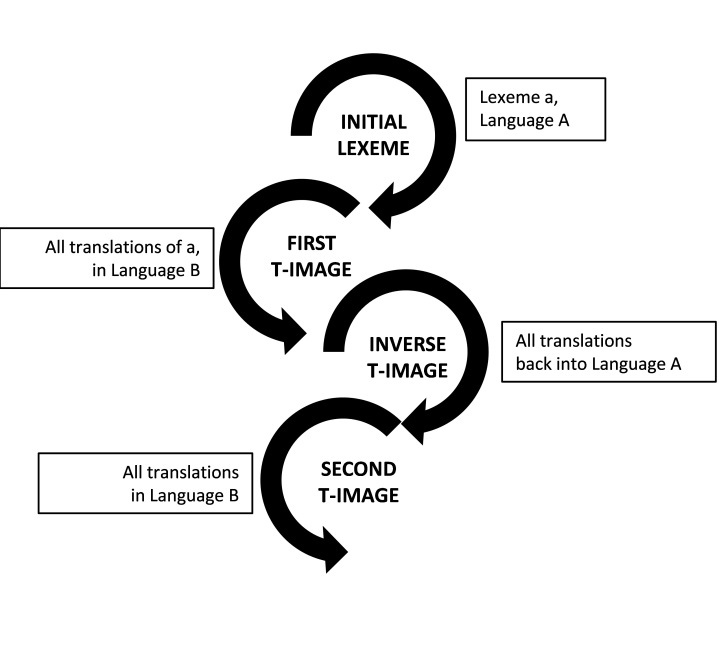
\includegraphics[height=.3\textheight]{figures/Vandevoorde2-img7.jpg}
\caption{\label{fig:key:8}  Work flow of the SMM}
\end{figure}

\subsection{Prerequisites and assumptions}
\label{sec:3.4.2}
A practical prerequisite to carry out the technique is that the researcher needs to have access to a parallel corpus, which is preferably at least sentence-aligned. If the corpus is word-aligned, the researcher can work in the most optimal circumstances (but word-alignment can be carried out manually or (semi-)automatically on the parallel sentences under investigation).

From the corpus which has been chosen, the researcher needs to be able to extract a set of alternative translations for each lemma one wishes to investigate \citep[31]{langemets_translations_2005}. After the application of the different steps of the SMM, this will ultimately create a “network of translational correspondences uniting the vocabularies of the two languages” (Ibid.)\todo{Fix ref}. Based on Dyvik’s ideas, and based on the following assumptions (verbatim from \citealt[31-32]{langemets_translations_2005}) “each language [will be used] as the ‘semantic mirror’ of the other”. The assumptions Dyvik puts forward are as follows:

\begin{itemize}
\item
Semantically closely related words tend to have strongly overlapping sets of translations.
\item
Words with wide meanings tend to have a higher number of translations than words with narrow meanings.
\item
If a word \textit{a} is a hyponym of a word \textit{b} (such as \textit{tasty} of \textit{good}, for example), then the possible translations of \textit{a} will probably be a subset of the possible translations of \textit{b.}
\item
Contrastive ambiguity, i.e., ambiguity between two unrelated senses of a word, such as the two senses of the English noun \textit{band} (‘orchestra’ and ‘piece of tape’), tends to be a historically accidental and idiosyncratic property of individual words. Hence we don’t expect to find instances of the same contrastive ambiguity replicated by other words in the language or by words in the other languages. (More precisely, we should talk about ambiguous \textit{phonological/graphic} words here, since such ambiguity is normally analysed as homonymy and hence as involving two lemmas.)
\item
Words with unrelated meanings will not share translations into another language, except in cases where the shared (graphic/phonological) word is contrastively ambiguous between two unrelated meanings. By assumption (4) there should then be at most one such shared word \citep[31-32]{langemets_translations_2005}.
\end{itemize}

\subsection{Overlap}
\label{sec:3.4.3}
When the SMM is applied to an initial lexeme, three types of word sense relationships can arise: “related word senses”, “unrelated word senses” and “mutually unrelated word senses” \citep[32]{langemets_translations_2005}. The first step that needs to be taken, is to isolate the mutually unrelated senses of each word (Ibid.)\todo{Fix ref} for which the resulting lexemes of the first T-image are used. I will try to illustrate the difference between related word senses, unrelated word senses and mutually unrelated word senses with the example of the Dutch word \textit{bank} (\figref{fig:key:9}), which can be translated in French as \textit{institution} \textit{financière} [financial institution], \textit{banque} [financial institution], \textit{banc} [seat] and \textit{fauteuil} [armchair]. This distinction between the different types of senses presented in the following sub-sections is based on Dyvik’s procedure for word sense isolation.

\begin{figure}\footnotesize
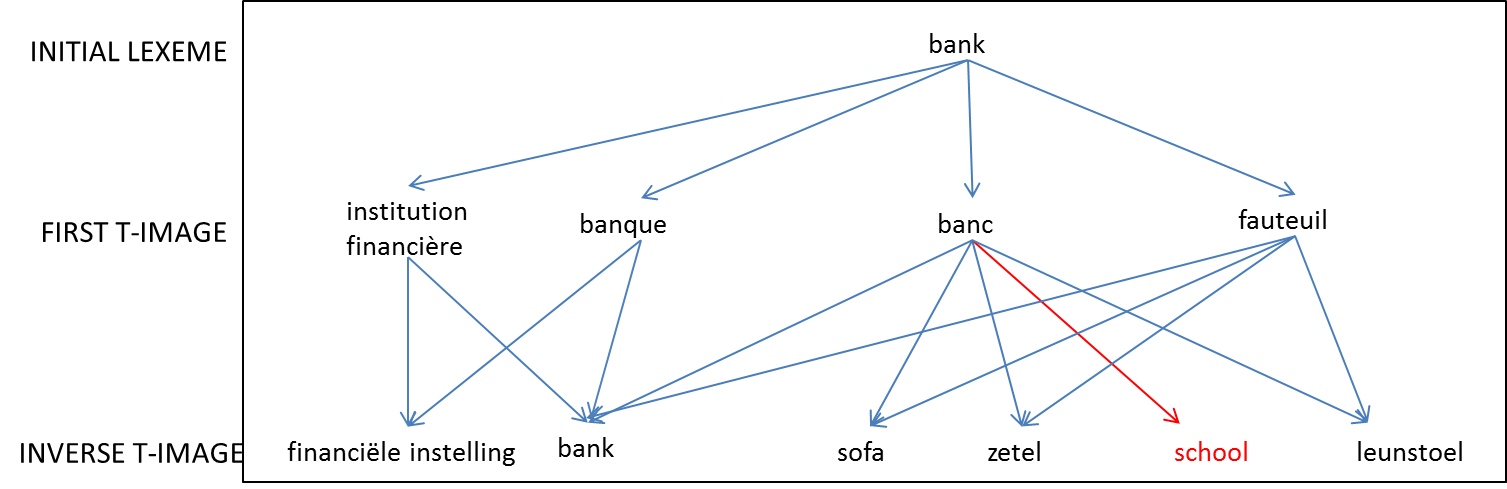
\includegraphics[height=.3\textheight]{figures/Vandevoorde2-img8.png}
\begin{tikzpicture}
    \matrix (SMM) [draw,matrix of nodes,nodes in empty cells,row 3 column 5/.style=red,row sep=1cm,column sep=2em] {
        \phantom{institution financière} & & bank & & & \\
        institution financière & banque & & banc & & fauteil\\
        financiële instelling & bank & sofa & zetel & [color=red]school & leunstoel\\
    };
    \foreach \i in {1,2,4,6} \draw[->] (SMM-1-3.south) -- (SMM-2-\i);
    \path[->] (SMM-2-1.south) edge (SMM-3-1)
                              edge (SMM-3-2);
    \path[->] (SMM-2-2.south) edge (SMM-3-1)
                              edge (SMM-3-2);                              
    \path[->] (SMM-2-4.south) edge (SMM-3-2)
                              edge (SMM-3-3)
                              edge (SMM-3-4)
                              edge [color=red] (SMM-3-5)
                              edge (SMM-3-6);
    \path[->] (SMM-2-6.south) edge (SMM-3-2)
                              edge (SMM-3-3)
                              edge (SMM-3-4)
                              edge (SMM-3-6);
    \node[left=.5cm of SMM-1-1.west,] {\scshape initial lexeme};
    \node[left=.5cm of SMM-2-1.west,] {\scshape first t-image};
    \node[left=.5cm of SMM-3-1.west,] {\scshape inverse t-image};
\end{tikzpicture}
\caption{\label{fig:key:9}Example of the (ficticious) SMM of \textit{bank}}
\end{figure}

\subsubsection{Unrelated word senses}
\label{sec:3.4.3.1}
The set of translations back into Dutch (the inverse T-image) of \textit{banque} and \textit{banc} only share the initial lexeme \textit{bank} itself in the inverse T-image. \textit{Banque} (\figref{fig:key:10}) is connected in the inverse T-image (i.e. ‘can be translated back into Dutch as’) to \textit{bank} and \textit{financiële} \textit{instelling.} As a consequence, it could be stated that the inverse T-image\textit{s} \textit{bank} and \textit{financiële} \textit{instelling} are semantically related to each other (via \textit{banque})\textit{:}

\begin{figure}
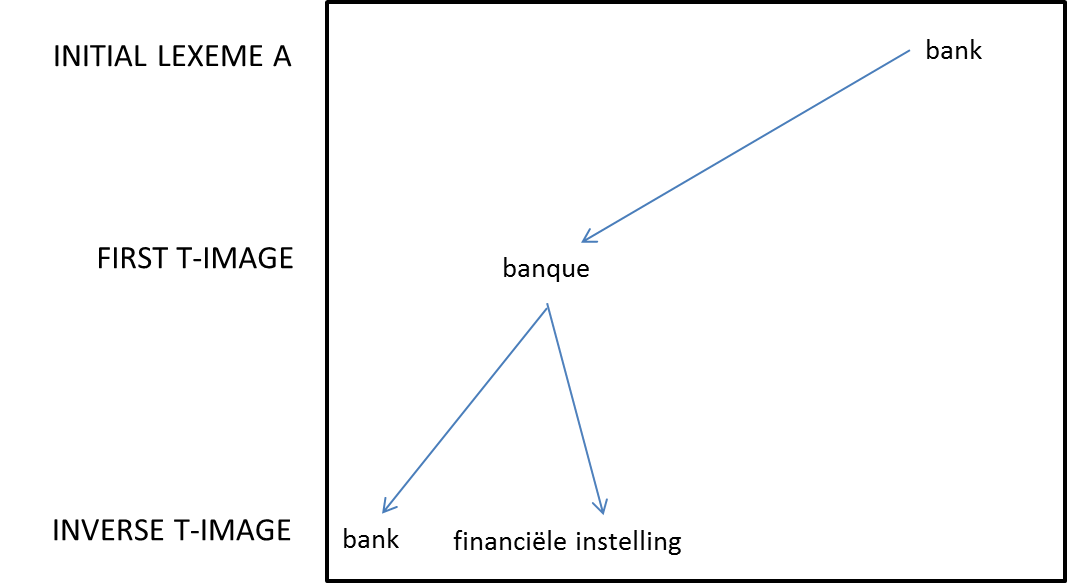
\includegraphics[height=.3\textheight]{figures/Vandevoorde2-img9.png}
\begin{tikzpicture}
    \matrix (SMM) [draw,matrix of nodes,nodes in empty cells,row sep=1cm,column sep=2em] {
        & & bank\\
        & banque &\\
        bank & financiële instelling &\\
    };
    \draw[->] (SMM-1-3) -- (SMM-2-2);
    \draw[->] (SMM-2-2) -- (SMM-3-1);
    \draw[->] (SMM-2-2) -- (SMM-3-2);
    \node[left=1cm of SMM-1-1.center,] {\scshape initial lexeme a};
    \node[left=1cm of SMM-2-1.center,] {\scshape first t-image};
    \node[left=1cm of SMM-3-1.center,] {\scshape inverse t-image};
\end{tikzpicture}
\caption{\label{fig:key:10}{Inverse} {T-image} {of} {banque}}
\end{figure}

\textit{Banc} (\figref{fig:key:11}) on the other hand, is connected in the inverse T-image to \textit{bank,} \textit{sofa,} \textit{zetel} and \textit{leunstoel,} which means that the inverse T-image lexeme \textit{bank} is semantically related to the other inverse T-image lexemes \textit{sofa,} \textit{zetel} and \textit{leunstoel} (via \textit{banc})\textit{:}

\begin{figure}
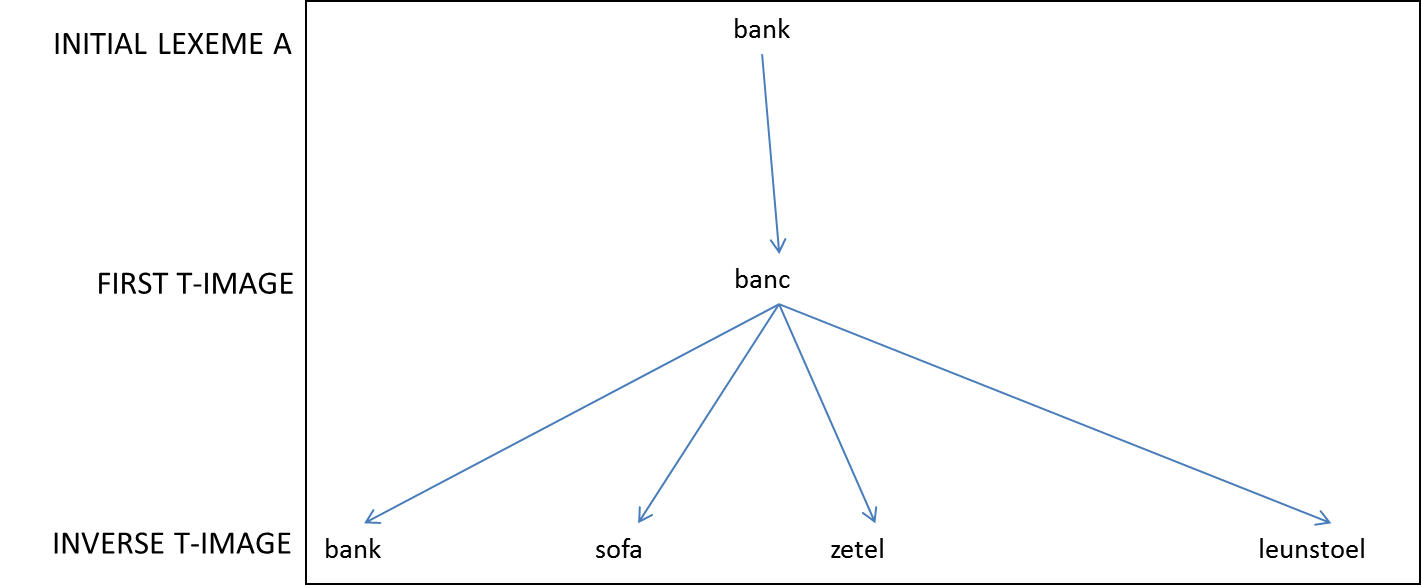
\includegraphics[height=.3\textheight]{figures/Vandevoorde2-img10.png}
\begin{tikzpicture}
    \matrix (SMM) [draw,matrix of nodes,nodes in empty cells,row sep=1cm,column sep=2em] {
        & bank & &\\
        & banc & &\\
        bank & sofa & zetel & leunstoel\\
    };
    \draw[->] (SMM-1-2) -- (SMM-2-2);
    \foreach \i in {1,2,3,4} \draw[->] (SMM-2-2) -- (SMM-3-\i);
    \node[left=1cm of SMM-1-1.center,] {\scshape initial lexeme a};
    \node[left=1cm of SMM-2-1.center,] {\scshape first t-image};
    \node[left=1cm of SMM-3-1.center,] {\scshape inverse t-image};
\end{tikzpicture}
\caption{\label{fig:key:11}Inverse T-image of \textit{banc}}
\end{figure}

The first T-images \textit{banque} and \textit{banc} only share \textit{bank} on the level of the inverse T-image, so \textit{banque} and \textit{banc} are “not directly connected by means of intersections with other sets” \citep[32]{langemets_translations_2005} indicating that their semantic relatedness cannot be proven (and that Dutch \textit{bank} is contrastively ambiguous between French \textit{banque} [financial institution] and \textit{banc} [seat]). This observation corresponds with Dyvik’s assumption (4): the Dutch lexeme \textit{bank} is indeed \textit{homonymous} between \textit{bank} [financial institution] and \textit{bank} [seat]. There is also evidence here for Dyvik’s assumption (5): the words \textit{banque} and \textit{banc} indeed only share (“at most”) one word (translation) at the level of the inverse T-image, i.e. the contrastively ambiguous \textit{bank.} Hence, an initial lexeme (e.g. \textit{bank}) possesses two distinct, unrelated senses (e.g. [financial institution] and [seat]) if the only shared word between their two sets of lexemes in the inverse T-image is the initial lexeme (which is the case here: the two sets only share \textit{bank}).

\subsubsection{Related word senses}
\label{sec:3.4.3.2}
Looking at the first T-images \textit{banc} and \textit{fauteuil} (Figures 12 and 13), we see that \textit{banc} is connected to \textit{bank,} \textit{sofa,} \textit{zetel} and \textit{leunstoel} in the inverse T-image (\figref{fig:key:12}), and that \textit{fauteuil} is connected to \textit{bank,} \textit{sofa,} \textit{zetel} and \textit{leunstoel} in the inverse T-image (\figref{fig:key:13}). In their inverse T-images, \textit{banc} and \textit{fauteuil} share, apart from \textit{bank}, also \textit{sofa,} \textit{zetel} and \textit{leunstoel}. \textit{Banc} and \textit{fauteuil} are thus directly connected by means of intersections with other sets: they do not only share \textit{bank} in the inverse T-image, they also share \textit{sofa,} \textit{zetel} and \textit{leunstoel}, proving the closer semantic relatedness of \textit{banc} and \textit{fauteuil}, and also showing that \textit{bank,} \textit{sofa,} \textit{zetel} and \textit{leunstoel} are semantically related.

\todo[inline]{Fig 3.5 and 3.4 are duplicates?}
\begin{figure}
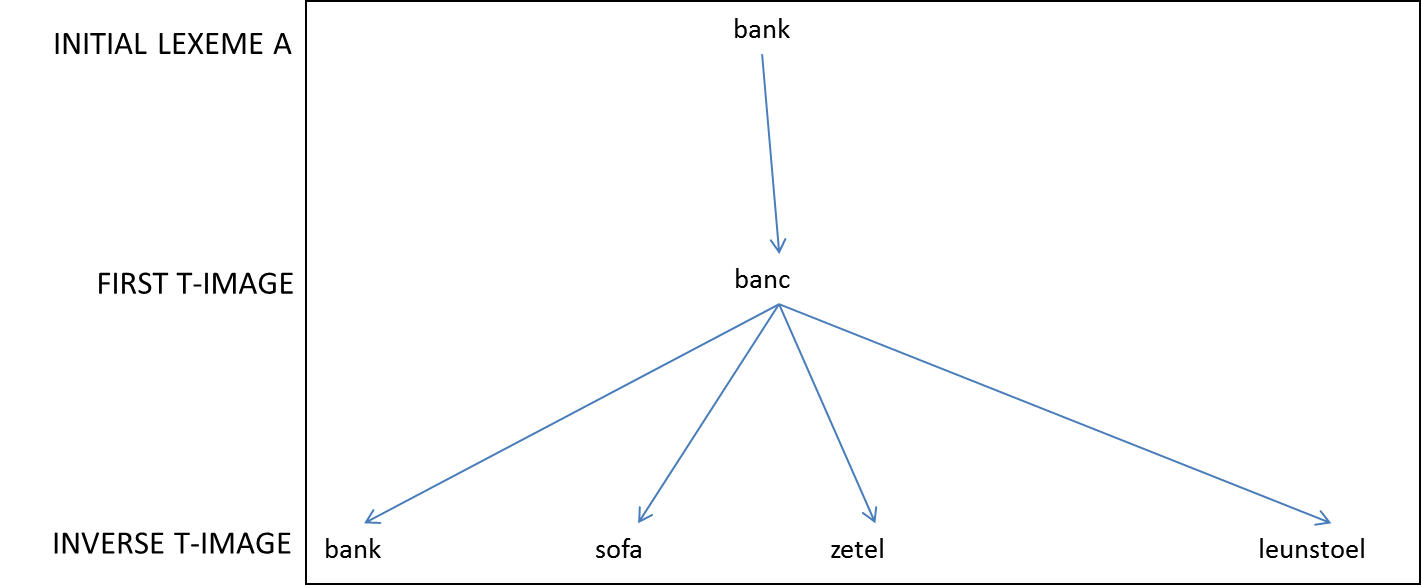
\includegraphics[height=.3\textheight]{figures/Vandevoorde2-img11.png}
\caption{\label{fig:key:12}  Inverse T-image of \textit{banc}}
\end{figure}

\begin{figure}
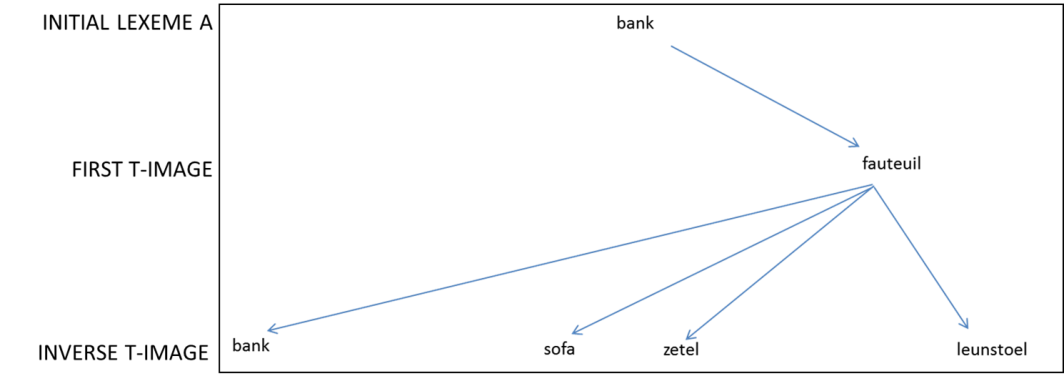
\includegraphics[height=.3\textheight]{figures/Vandevoorde2-img12.png}
\begin{tikzpicture}
    \matrix (SMM) [draw,matrix of nodes,nodes in empty cells,row sep=1cm,column sep=2em] {
        & bank & &\\
        &  & & fauteuil\\
        bank & sofa & zetel & leunstoel\\
    };
    \draw[->] (SMM-1-2) -- (SMM-2-4);
    \foreach \i in {1,2,3,4} \draw[->] (SMM-2-4) -- (SMM-3-\i);
    \node[left=1cm of SMM-1-1.center,] {\scshape initial lexeme a};
    \node[left=1cm of SMM-2-1.center,] {\scshape first t-image};
    \node[left=1cm of SMM-3-1.center,] {\scshape inverse t-image};
\end{tikzpicture}
\caption{\label{fig:key:13}  Inverse T-image of \textit{fauteuil}}
\end{figure}

\subsubsection{Mutually unrelated word senses}
\label{sec:3.4.3.3}
A final possible scenario concerns the example of the Dutch word \textit{school} [school] in the inverse T-image (look back at \figref{fig:key:9}, the example of the (fictitious) SMM of \textit{bank).} Dutch \textit{school} [school] is a possible translation back into Dutch of the French first T-image word \textit{banc,} in its meaning [school of fishes]. But this latter meaning [schoo] is not a meaning of Dutch \textit{bank}. Without any knowledge of Dutch and French, the unrelatedness can be deduced from the translational relation\textit{:} \textit{school} is only translationally related to its French source lexeme \textit{banc}, but it is not related to \textit{bank} on the level of the inverse T-image, implying that the senses of \textit{bank} and \textit{school} are mutually unrelated (\figref{fig:key:14}). Whereas unrelated senses shared only their initial lexeme in the inverse T-image \textit{–} enabling a distinction between unrelated senses of the initial lexeme \textit{bank}; mutually unrelated senses such as \textit{school} and \textit{bank} are not at all related to each other in the inverse T-image.

\begin{figure}
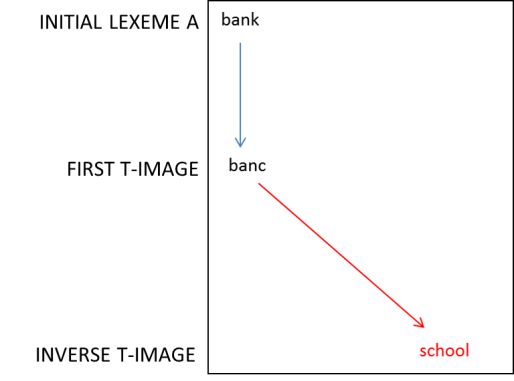
\includegraphics[height=.3\textheight]{figures/Vandevoorde2-img13.png}
\begin{tikzpicture}
    \matrix (SMM) [draw,matrix of nodes,nodes in empty cells,row sep=1cm,column sep=2em,row 3 column 2/.style={red}] {
         bank &\\
         banc &\\
         & school\\
    };
    \draw[->] (SMM-1-1) -- (SMM-2-1);
    \draw[->,color=red] (SMM-2-1) -- (SMM-3-2);
    \node[left=1cm of SMM-1-1.center,] {\scshape initial lexeme a};
    \node[left=1cm of SMM-2-1.center,] {\scshape first t-image};
    \node[left=1cm of SMM-3-1.center,] {\scshape inverse t-image};
\end{tikzpicture}
\caption{\label{fig:key:14}  Mutually unrelated sense \textit{school}}
\end{figure}

\subsubsection{Word sense individuation}
\label{sec:3.4.3.4}
The individuation of word senses can now take place: one of the meanings of \textit{bank} [financial institution] can be expressed by \textit{bank} and \textit{financiële} \textit{instelling,} another meaning of \textit{bank} [seat] can be expressed by \textit{bank,} \textit{sofa,} \textit{zetel,} \textit{leunstoel}. \textit{School} is not a sense of the initial lexeme \textit{bank} and should be disregarded for the further investigation of the senses of \textit{bank.} Dyvik summarizes the principle on which the isolation of word senses takes place as follows:

\begin{quote}
In our translational approach, the semantic fields are isolated on the basis of \textit{overlapping} \textit{t-images}\textbf{ }[first T-images]\textit{:} two senses belong to the same semantic field if they have intersecting first t-images (after sense individuation one member in the intersection is sufficient), or if there is a sequence of such intersecting t-images [first T-images] joining them (\citealt[33]{langemets_translations_2005}, my emphasis, my own terminology is added between brackets for clarity’s sake).
\end{quote}

If one is interested in studying one specific semantic field, a criterion of overlapping (first) t-images or overlap can be observed, meaning that a lexeme at the level of the inverse T-image is only selected when it is related to at least two lexemes on the level of the first T-image. In this way, for the example of \textit{bank,} we see that \textit{school} is linked to only one lexeme on the level of the first T-image viz. \textit{banc}. \textit{School} does not meet the overlap criterion, which is an indication that it pertains to a different semantic field. As for \textit{sofa,} for example, we see that it is linked to both \textit{banc} and \textit{fauteuil} on the level of the first T-image, proving that it pertains to the semantic field under scrutiny.

By consequence, by taking into account a criterion of overlap between the inverse T-image lexemes and the first T-image lexemes (every lexeme selected on the level of the inverse T-image must be a translation of at least two first T-image lexemes), it is guaranteed that mutually unrelated senses are excluded. If words without overlap were included in the analysis (i.e. words which are not related to at least two lexemes on the level of the first T-image), the result of the SMM would risk to contain senses which are mutually unrelated, meaning that they are in fact not a sense of the word under study.

\subsubsection{Necessity of overlap}
\label{sec:3.4.3.5}
The previous paragraphs have shown that overlap is a crucial notion for the selection of those lexemes which pertain to the same semantic field. It has also been shown that the existence of more than one translation for a given word is not a sufficient argument to accept that the word is ambiguous \citep[30]{langemets_translations_2005}. In fact, it only implies that the denotation of the word spans the denotations of two words in a different language (p.29). This observation has important implications for the use of the translational relation for meaning investigation: “non-transitive translational connections may tie together semantically distant words in the same semantic field” (Ibid.)\todo{Fix ref} – as we have shown in the example of \textit{school}. Dyvik makes an important point about the use of back-translation in this regard\textit{:} the translational relation should be used with care when it is applied for the establishment of semantic relatedness, and overlap is a necessary criterion if one wants to ‘confine’ a semantic field. This problem has also been observed in computational linguistics, where it is generally solved by the addition of another language \citep{gelbukh_five_2013}. The appearance of overlapping translations was already formulated by Ivir (see \sectref{sec:2.3.2} of this study: “each L\textsubscript{2} correspondent will be related to a number of other L\textsubscript{1} items too, besides the L\textsubscript{1} with which the analysis was initiated”) but Ivir did, to my knowledge, never exploit this idea explicitly as a validation of the semantic relatedness between the lexemes of a semantic field. Dyvik’s point about the semantic informativity of translations makes his technique directly applicable for lexical semantic research. His reflection about what happens to both ambiguous and unrelated senses when the translational relation is used via back-translation furthermore offers useful insights into what exactly happens when one utilizes translation for meaning-informative tasks.


\section{Extended Semantic Mirrors Method: SMM++}
\label{sec:3.5}
The goal of this methodological chapter is to find an adequate way to retrieve lexemes as candidate-members of a semantic field under scrutiny for both non-translated (original/source) language and translated (target) language and to arrive at comparable visualizations of semantic fields of a same initial lexeme in both translated and non-translated language. The SMM developed by Dyvik, and some of the additions proposed by contrastive linguists who applied the technique answer the retrieval\textbf{ }question: by going back and forth between sources and translations, and by creating new sets of data at every stage of the exercise, a set of candidate-lexemes of a semantic field can be obtained. The SMM is an expansive, meaning informative technique which can be used for the retrieval of lexemes pertaining to a semantic field.

In order to provide a ‘complete’ methodological answer, the SMM will still need to undergo a few extensions. The SMM can indeed help to retrieve candidate-lexemes for a semantic field, but in order to implement Dyvik’s technique as a methodological tool to investigate translational phenomena – via a comparison of semantic fields of translated and non-translated language – a number of issues need to be dealt with.

In this section, I will propose two extensions of the SMM\footnote{The two extensions to the SMM in \sectref{sec:3.5.1} and \sectref{sec:3.5.2} were first introduced and described in a less elaborate way in \citet{vandevoorde_corpus-based_2017}, an article which is under copyright. Its publisher should be contacted for permission to re-use or reprint the material in any form.}. The first extension is concerned with the integration of translation direction and the asymmetry of translation into the retrieval task (\sectref{sec:3.5.1}); the second extension we will focus on how the output of the retrieval task can be used as an input for a statistical visualization of a semantic field (\sectref{sec:3.5.2}).

\subsection{Extension 1: Translation direction and asymmetry of translation}
\label{sec:3.5.1}
In the SMM, the translational relation is considered as symmetric, i.e. a relation which exists irrespective of the translation direction. The second T-image results in a set of Language B lexemes which are translations into Language B of the Language A lexemes from the inverse T-image. The second T-image provides the necessary information to establish a semantic field in Language B, just as the resultant information from the inverse T-image (translations into Language A of the Language B lexemes from the first T-image) permits the establishment of a semantic field in Language A, and “paired semantic fields in the two languages involved” \citep[33]{langemets_translations_2005} are created.

For the translation studies scholar, accepting the symmetry of the translational relation would be refuting almost the totality of the existing research tradition in translation studies. When integrating the SMM for research in TS, one inevitably has to take into account the asymmetric nature of the translational relation as well as the reality of translation direction. This implies that, in my view, translation – as an activity which forms the subject of research in TS – always happens in the direction from a source language into a target language. Differentiating between source and target language does matter in TS, for it is precisely the influence of either source or target language (or both) on the process and the final product of translation which is a pending subject of research in TS.

Two sets of data are therefore created, which can form the basis for a comparison of a semantic field of a lexeme under scrutiny: one data set representing non-translated (original/source) language (in this case non-translated Dutch), and a second data set representing translated (target) language (in this case translated Dutch with English or French as a source language).

Non-translated Dutch and translated Dutch need to be represented by separate sets of data, which furthermore need to be (easily) comparable. In addition to that, the semantic fields created on the basis of these data sets need to consist of lexemes in the same language as the initial lexeme (Dutch). \tabref{tab:key:1} below shows the original structure of the SMM as it was conceived by Dyvik. In the fourth column, translation direction is added. Suppose an SMM is carried out on an initial lexeme \textit{a} in language A, for which language A is Dutch and language B is English, then the following scheme applies:

\begin{table}\caption{\label{tab:key:1} Source and target language in the different steps of the SMM}
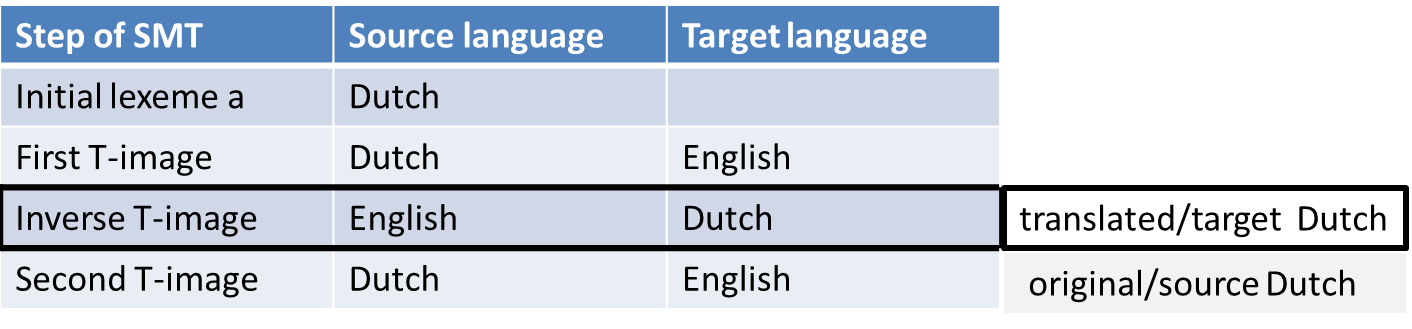
\includegraphics[height=.3\textheight]{figures/Vandevoorde2-img14.png}
\end{table}
  
From this \tabref{tab:key:1}, it becomes clear that Dutch (Language A) is a source language in the first and the second T-image and a target language in the inverse T-image. This implies that the data sets which are yielded by the different steps of the SMM are different in translational nature\textit{:} the data set retrieved at the level of the inverse T-image can be used to analyze translated (target) Dutch, whereas the data set retrieved at the level of the second T-image can be utilized to analyze non-translated (original/source) Dutch.

The first extension thus consists in a differentiation between sets of retrieved data within the different steps of the SMM based on their translational status (source or target language). Instead of using the second T-image to make a contrastive comparison (like Dyvik) or disregarding it (like \citealt{aijmer_model_2004}), I assign a new role to this step of the SMM, based on the translational status of the data. This is a necessary first step to make the data obtained via the SMM usable for TS research. Further references in this book to translated language, will be written as TransLanguage\textsubscript{A} (in this study TransDutch\textsubscript{ENG} and TransDutch\textsubscript{FR}); referring to the sets of data obtained in the inverse T-image with a Language B (in our study English or French) as a source language and any Language A (in our study Dutch) as a target language. References to non-translated (original/source) language, will be written as SourceLanguage\textsubscript{A} (in this study SourceDutch); the underlying data set will be the one obtained in the second T-image with any language A (in this study Dutch) as a source language and any Language B (here: English or French) as a target language.

\subsection{Extension 2: Statistical implementability of the data sets}
\label{sec:3.5.2}
In the previous section, I dealt with the asymmetric nature of translation and determined a way to compile sets of translated and non-translated language by extending the existing SMM. The next step is to arrive at comparable visualizations of those sets of lexemes. The information which has so far been obtained only gives the researcher sets of lexemes, but does not propose any kind of organization of those lexemes which could give further information about the semantic relatedness between the lexemes.

Within the original SMM, hierarchical patterns are “only based on overlap relations among \textit{t-}images” and are obtained by ranking the lexemes “independently of frequency of occurrence” \citep[73]{johansson_translational_1998}. The degree of semantic similarity between the lexemes in the created hierarchy is only based on the number of overlapping translations while frequency information is excluded. \tabref{tab:key:2} shows a fictitious example of the translational relation in the inverse T-image of Dutch \textit{bank} with French as a pivot language. Based on this information, and following Dyvik, the centrality of \textit{bank} in a field with \textit{bank,} \textit{financiële} \textit{instelling,} \textit{sofa} and \textit{leunstoel} could be deduced from the fact that bank is a translation of all three French lexemes \textit{banque,} \textit{banc} and \textit{fauteuil}.

A visualization based solely on overlapping t-images is usually realized via Venn diagrams \citep{dyvik_semantic_2011}, which tend to get rather complex to interpret. This apparent weak point of the SMM has led computational linguists to propose different methods of visualization which can be of use for computational research purposes (see e.g. \citealt{ganter_conceptual_2005}). It is not in the scope of this book to computationally implement the SMM. However, the objective to create visualizations which can provide more insights into the alleged semantic differences between translated and non-translated language on the basis of the SMM, implies the use of methods more closely connected to distributional semantics. Within that framework, the typical approach is to collect occurrence counts of words and other words/features in a frequency table. The reason is that frequencies indicate the strength of certain relations, i.e. they will tell us which patterns are important. Such frequency tables can be thought to represent translated language when the translated lexemes are represented as rows with their source language lexemes as column variables. They can represent non-translated language when the non-translated (source language) lexemes are represented as rows with their translations as column variables. The integration of frequency information is the second major extension to the SMM. If frequency information is now integrated into the previously given fictitious example of bank, the result looks as follows for non-translated (original/source) language bank (\tabref{tab:key:3}) and translated (target) language bank (\tabref{tab:key:4}).

\begin{table}\caption{Overlapping translations of bank (ficticious) in the inverse T-image\label{tab:key:2}}
\begin{tabularx}{\textwidth}{lXXXX}
\lsptoprule
%%[Warning: Draw object ignored]
{is} {translated} {as} & {bank\textsubscript{[nl]}} & {financiële} {instelling\textsubscript{[nl]}} & {sofa\textsubscript{[nl]}} & {leunstoel\textsubscript{[nl]}}\\\midrule
{banque\textsubscript{[fr]}} & \Checkmark & \Checkmark & \XSolidBrush & \XSolidBrush\\
{banc\textsubscript{[fr]}} & \Checkmark & \XSolidBrush & \Checkmark & \Checkmark\\
{fauteuil\textsubscript{[fr]}} & \Checkmark & \XSolidBrush & \Checkmark & \Checkmark\\
\lspbottomrule
\end{tabularx}
\end{table}

\begin{table}
\caption{Frequency table for original bank – second T-image (fictitious)\label{tab:key:3}}
\begin{tabularx}{\textwidth}{Xrrr}
\lsptoprule
{is} {translated} {n} {times} {as} & {banque\textsubscript{[fr]}} & {banc\textsubscript{[fr]}} & {fauteuil\textsubscript{[fr]}}\\\midrule
{bank\textsubscript{[nl]}} & 231 & 61 & 45\\
{financiële} {instelling\textsubscript{[nl]}} & 178 & 0 & 0\\
{sofa\textsubscript{[nl]}} & 0 & 124 & 32\\
{leunstoel\textsubscript{[nl]}} & 0 & 27 & 76\\
\lspbottomrule
\end{tabularx}
\end{table}

\begin{table}
\caption{Frequency table for translated bank - \textit{inverse} \textit{T-image} (fictitious)\label{tab:key:4}}
\begin{tabularx}{\textwidth}{Xrrr}
\lsptoprule
{is} {n} {times} a translation of & {banque\textsubscript{[fr]}} & {banc\textsubscript{[fr]}} & {fauteuil\textsubscript{[fr]}}\\\midrule
{bank\textsubscript{[nl]}} & 230 & 32 & 45\\
{financiële} {instelling\textsubscript{[nl]}} & 121 & 0 & 0\\
{sofa\textsubscript{[nl]}} & 0 & 98 & 32\\
{leunstoel\textsubscript{[nl]}} & 0 & 67 & 43\\
\lspbottomrule
\end{tabularx}
\end{table}

The occurrence counts in the frequency tables implicitly also contain the number of overlapping translations (or source language lexemes). Hence, the frequency tables contain information about both the frequency of co-occurrence of each source language lexeme (or translation) with each translation (or source language lexeme) as well as overlap information about which translations (or source language lexemes) are attested for each source language lexeme (or translation). Advanced statistical techniques can now be applied upon the data sets, opening the way to statistical visualization techniques such as Correspondence Analysis \citep{greenacre_correspondence_2007,lebart_exploring_1998} and Hierarchical Cluster Analysis (\citealp[138]{baayen_analyzing_2008};\citealp[336]{gries_statistics_2013}), a technique that will allow for a visual representation of the similarities and differences between the sets of lexemes. Previous research in Contrastive Linguistics has shown that Hierarchical Cluster Analysis is an excellent tool for the evaluation of corpus-based, lexico-semantic analyses \citep{evans_behavioral_2009,libben_behavioral_2012,glynn_cluster_2014}.


\subsection{Technical fine-tuning}
\label{sec:3.5.3}
Although the integration of frequency information into the SMM makes it possible to process the results statistically, one problem still remains. SMM is an expansive technique, implying that, with every step, more and new information is generated, in this case: new translation solutions for the lexeme(s) are retrieved, and their number increases in every step of the mirror analysis. Although this effect is of course at the core of the technique, it also implies that the number of possible translation solutions grows exponentially with every step of the mirror analysis, leading to data sets which are difficult if not impossible (i) to manage manually or even semi-automatically and (ii) to compare with each other (depending on the initial lexeme in Language A one chooses or on the Language B one chooses, the SMM will select different lexemes).

First, let us take a closer look at the problem of how to manage these (ever) expanding data sets within the retrieval task of the SMM. Translators come up with very creative solutions, even in non-fictional, non-literary texts. For example, within a corpus study, this creativity results in the following: for a verb as ‘basic’ as \textit{beginnen} [to begin], more than 47 different translations in English appear for a total of 382 translational pairs of sentences with \textit{beginnen} in the Dutch source text in the Dutch Parallel Corpus. It can be very interesting, both from a contrastive linguistic as from a translational perspective, to investigate all these instances, but it would not answer one of the main research questions of this book: how to compare semantic relationships in translated language and non-translated language. For this reason, I agree with Dyvik to exclude completely unpredictable translations – translators’ idiosyncracies – from our analysis. More specifically, I will apply a frequency threshold of three attestations for every translation, allowing me to work with a manageable number of possible translational pairs. This choice is motivated by pragmatic considerations. Firstly, a frequency threshold below three attestations generates additional manual annotation work, endangering the feasibility of the task. Solutions such as automatic word alignment with GIZA++ did not yield satisfying results due to unsuficient corpus size, and word aligned parallel corpora are not available for the language pairs in this book. Secondly, with respect to the statistical processing of the data, Evert argues against the inclusion of hapax and dis legomena, providing an additional argument in favor of a frequency threshold of three observations:

\begin{quote}
[f]or the time being, however, we must assume that probability estimates and p-values for the lowest-frequency types are distorted in unpredictable ways. [...] these conclusions provide theoretical support for frequency cutoff thresholds. Data with cooccurrence frequency f < 3, i.e. the hapax and dis legomena, should always be excluded from the statistical analysis \citep[133]{evert_statistics_2004}.
\end{quote}

A second restriction of the data is necessary to make sure that the data sets are also acceptably comparable. I will therefore respect the following rule of selection for data at the level of the second T-image (representing non-translated language): in the second T-image, an observation (source-target sentence pair holding the lexeme under investigation) will only be selected when the Language B translation is identical to one of the Language B source language lexemes of the inverse T-image (representing translated language). As a result, the row names and column variables of the data matrices in the inverse T-image (representing translated language) and the second T-image (representing non-translated language) will be identical, their difference will lay in their status. In the frequency table representing non-translated language (SourceDutch), the rows are (Dutch) source language lexemes and the columns are (English or French) translations, in the frequency table representing translated language (TransDutch\textsubscript{ENG} or TransDutch\textsubscript{FR}), the rows are (Dutch) translations and the columns are (English or French) source language lexemes. Of course, the frequency counts in the tables will also be different (as illustrated by the difference between \tabref{tab:key:3} and \tabref{tab:key:4} for the fictitious example of \textit{bank}). A similar restriction was also suggested by \citet[60]{johansson_translational_1998} in order to eliminate those results which are unrelated to the initial lexeme. Shortly put: the lexemes which are members of each of the data sets selected for statistical analysis and further visualization are kept identical (the inverse T-image provides the lexemes for the semantic field of translated language, and the second T-image provides the lexemes for the semantic field of non-translated language), but the ‘content’ (frequency information and translational status) of the data sets differs since source and target language are in fact inversed in the two sets of data. In this way, we solve the semantic paradox of \citet{krzeszowski_contrasting_1990} which we are facing here that “what is identical is not subject to comparison, and what is different is not comparable” \citep[7]{krzeszowski_contrasting_1990}: we propose to select identical lexemes, but because of their translational status, both data sets are nonetheless different; solving the paradox and making the two sets of data comparable to each other.

Conclusively, the previously mentioned adjustments will lead to (i) a selection of a manageable amount of manually controlled data on which a quantitative analysis can be carried out and (ii) the comparability of the two data sets.

\subsection{Conceptual issue}
\label{sec:3.5.4}
The application of the SMM++ leads to the creation of comparable data sets of translated and non-translated language. The frequency tables are obtained on the basis of translational data and following a translation-based method. For the data set of non-translated (source) language, both the nature of the data as well as the nature of the method could well be held against it. In this section, I will show that it can be made conceptually acceptable to use translational data and a translation-based method to obtain a frequency table for non-translated language.

One of the basic assumptions when implementing a method such as the SMM is exactly the idea that the translational relationship can be used as an analytical basis, i.e. to consider “sets of translationally corresponding items across languages as the primitives of semantic descriptions” \citep[31]{langemets_translations_2005}. As a consequence, the translations which are generated by the SMM in the pivot language(s) can be considered as analogous to semantic features. These semantic primitives or semantic features are similar to the attributes of the prototype-based theory on semantic organization we presented in \chapref{sec:2}. Under the assumption that translations can indeed constitute a kind of attribute, a semantic description on the basis of translations becomes acceptable and the visualization of non-translated language on the basis of translations (as semantic features) becomes defensible too. The fact that different languages carve up the world in different ways is used to the advantage of the proposed method: contrastive differences can be seen as a reflection of difference(s) (in classification) of semantic properties and can consequently be semantically informative.

As explained in \sectref{sec:3.5.1}, the corpus observations which are selected to investigate non-translated (source) language are source language data. As a consequence, translation cannot have affected the use of a specific source language lexeme in its non-translated environment simply because it is not translated. The use of source language data to represent non-translated data is, in my opinion, conceptually acceptable, but one should keep in mind that the mere selection of a text as a source text, i.e. a text selected to be translated, does have a certain impact: some texts might be more often and more commonly selected for translation than others, whereas still others may have been excluded due to various factors, sometimes referred to as preliminary norms \citep{toury_descriptive_1995}. In addition, the lexeme selection method is and remains of course based on a translation-based technique, viz. the SMM++. While its translational nature assures the semantic relatedness, the ungraspable trace of the translational basis of the method on the selection of the lexemes needs to be accepted. One could argue that monolingual data would better fit the purpose of visualizing non-translated language structure. Although this is a valid point, previous studies using monolingual reference corpora have faced major comparability issues due to corpus size or uncertainty about the (translational) status of the texts in the presumed original language corpora (e.g. \citealt{musolff_conceptual_2014}). Another option would be to base the visualizations on a different hypothesis which does not rely on translations as semantic features. If, for instance, the distributional hypothesis were applied, then only the monolingual contextual information of the Dutch source language sentences would have to be used for the visualization of non-translated language\footnote{\citet{vandevoorde_distributional_2016} show that semantic fields of \textit{beginnen}/inchoativity obtained via the distributional method are similar to those obtained via the translational method.}.

Some additional steps to keep the possible source language influence to a minimum are taken, ensuring a ‘fair’ comparison between original language and translated language using the same technique, the same hypothesis and the same data. As a first precautionary measure, I will refer to these data sets and their subsequent visualizations as SourceLanguage\textsubscript{A} instead of OriginalLanguage\textsubscript{A}. Secondly, I will combine the data of two semantic mirrors for the SourceLanguage\textsubscript{A} data set. This means that the semantic features from two distinct languages will be combined for the visualization of SourceLanguage\textsubscript{A}. In this way, I maximize the neutralization of any possible specific influence of the semantic features (translations) on the visualization of SourceLanguage\textsubscript{A}.

\section{Applying the first extension of the SMM to retrieve data sets for beginnen}
\label{sec:3.6}
In this section, the SMM++ retrieval task is applied to obtain data sets which can represent the semantic field of \textit{beginnen}/inchoativity in Dutch. The corpus which was used to retrieve the data is the Dutch Parallel Corpus (see \sectref{sec:3.3}). I will describe how the three resultant data sets were obtained by applying the SMM++ to the initial lexeme \textit{beginnen} in the DPC. One data set is obtained for non-translated Dutch (SourceDutch) and two data sets for translated Dutch, one with English as a Language B (TransDutch\textsubscript{ENG}) and a second one with French as a Language B (TransDutch\textsubscript{FR}). All data sets were retrieved following the exact procedure described above. \textit{Beginnen} was chosen as the initial lexeme, because it can be considered as the most prototypical expression of inchoativity: it is used more frequently than its closest near-synonym \textit{starten} [to start] with 291,438 hits for \textit{beginnen} versus 23,986 for \textit{starten} in the Dutch reference corpus SONAR \citep{spyns_construction_2013}.

The first mirroring will be carried out with English as a Language B, the second mirroring with French as a Language B. The second T-image of \textit{beginnen} with English as a Language B and the second T-image of \textit{beginnen} with French as a Language B will be joined into one the data set SourceDutch. The inverse T-image of \textit{beginnen} with English as a Language B will result in the data set TransDutch\textsubscript{ENG}, the inverse T-image of \textit{beginnen} with French as a Language B will result in the data set TransDutch\textsubscript{FR}.

\subsection{ First T-images of beginnen\textsubscript{ENG}\textsubscript{} and beginnen\textsubscript{FR}}\footnotemark{}\label{sec:3.6.1} 
\footnotetext{ Beginnen\textsubscript{ENG} refers to the semantic mirroring initiated by the initial lexeme \textit{beginnen} and with English as a language B. Beginnen\textsubscript{FR} refers to the semantic mirroring initiated by the initial lexeme \textit{beginnen} and with French as a language B.}

The SMM++ was first carried out with English as a pivot language. Attestations of the Dutch verb \textit{beginnen} were queried in the DPC via the interface developed by \citet[62]{delaere_translations_2015}. A lemma-based query was carried out rendering all sentences with \textit{beginnen} in any of its inflected forms. From the 1,867 resulting observations, 382 fulfilled the criterion of translation direction (Dutch as a source language, English as a target language). Each of the 382 sentences was manually annotated, meaning that the translation of \textit{beginnen} was recorded for every sentence. For the example (1) below, \textit{take} \textit{up} was annotated as the translation of \textit{beginnen}:

\begin{itemize}
\item \begin{styleVoorbeeld}
SOURCE: Zo vermeldde iemand bijvoorbeeld: "Ongeveer 80 procent van de afgestudeerden van onze kunstacademie zal een carrière beginnen in de creatieve industrie". [Someone mentioned for example: “About 80 percent of the graduates of our academy of arts will begin a career in the creative industry”.]
\end{styleVoorbeeld}\end{itemize}
\begin{quote}
TARGET: For example, in one case "Around 80 percent of graduates from our art school will take up careers in the creative industries". (dpc-vla-001920-nl, our emphasis)
\end{quote}

From the 382 observations, 46 were disregarded for further analysis. Three reasons for elimination were distinghuised. Two of them apply to all data retrieval and annotation tasks in our study, the third one is specific to the case of \textit{beginnen} with English as a Language B.

\begin{itemize}
\item 
The sentence alignment is erroneous. In this case, it is technically possible to look up the complete texts from which the aligned sentences were extracted and re-align the sentence correctly. However, I chose to disregard the erroneously aligned sentences out of practical considerations.
\item 
The source language lexeme under consideration is not translated at all (or no translation equivalent can be indicated in a straightforward way). Observations where the lexeme under study remains untranslated in the target sentence, such as in the following example (2), are disregarded for further analysis:
\end{itemize}
\begin{itemize}
\item \begin{styleVoorbeeld}
SOURCE: Ondernemers begonnen koortsachtig op zoek te gaan naar snoeiposten, [...]. [Entrepreneurs feverishly began to look for targets for cut backs]
\end{styleVoorbeeld}\end{itemize}
\begin{styleVoorbeeld}
TARGET: Company managers feverishly grasped to make savings, [...] (dpc-ing-002337-nl, our emphasis)
\end{styleVoorbeeld}

Although it would as such be interesting to examine why the inchoative aspect disappeared from the target sentence, this question is not addressed in the current study.


\begin{itemize}
\item 
The third reason to eliminate an observation is when the lexeme \textit{beginnen} is non-lexicalized in translation. This case is particularly relevant to the translation of Dutch \textit{beginnen} into an English progressive structure (although similar translational situations are imaginable for this same verb and surely exist for other verbs, this is the only case encountered within our study of \textit{beginnen} with English and French as languages B). Consider the following example 3:
\end{itemize}
\begin{itemize}
\item \begin{styleVoorbeeld}
SOURCE: Terwijl de Europese Unie zich stilaan begint op te maken om 10 nieuwe lidstaten te verwelkomen, blijft de Europese economie een slappe bedoening . [While the European Union begins gradually to prepare itself to welcome 10 new member states, the European economy reamins a sluggish affair.]
\end{styleVoorbeeld}\end{itemize}
\begin{styleVoorbeeld}
  TARGET: While the European Union is gradually preparing to welcome 10 new member states, the European economy remains in the doldrums. (dpc-ing-001896-nl, our emphasis)
\end{styleVoorbeeld}


In this particular example \textit{zich} \textit{opmaken} is translated by \textit{to} \textit{prepare} and \textit{stilaan} is translated by \textit{gradually}. The verb \textit{beginnen} is not translated lexically here; instead its translation is couched in the structure ‘to be+ing-form’ applied to the verb \textit{to} \textit{prepare}. Observations where an inchoative verb is translated by the syntactic structure such to be+ing-form were excluded for further. Although annotation was perfectly possible on the technical side, the inchoative aspect of the structure ‘to be+ing-form’ is often very subtle \citep{smith_parameter_1997} and open for debate, as the following example (4) clarifies:


\begin{itemize}
\item \begin{styleVoorbeeld}
SOURCE: But thanks to technological advances, plasma techniques are playing an ever greater role in our daily life: just think of fluorescent tubes and flat screen televisions, for example.
\end{styleVoorbeeld}\end{itemize}
\begin{styleVoorbeeld}
TARGET: Dankzij de technologische ontwikkeling duiken steeds meer plasmatoepassingen op in ons dagelijks leven. Denken we maar aan de tl-lampen of aan het vlakke plasmascherm van televisietoestellen. [Thanks to technological development, more and more plasma applications are popping up in our daily live. Think of striplighting or the flat plasma screen of television sets.] (dpc-arc-002037-en, our emphasis).
\end{styleVoorbeeld}

In example 4, the pattern ‘to be+ing-form’ could arguably be said to carry an inchoative aspect. The Dutch target sentence in fact even provides evidence for the inchoative aspect: the verb \textit{to} \textit{play} is not translated into \textit{spelen}, which would have been a perfectly acceptable translation solution and even the readiest one (\textit{een} \textit{rol} \textit{spelen} [to play a role]). Instead, the translator selected the verb \textit{opduiken} [to pop up, to turn up] which lexicalizes the inchoative aspect of the ‘to be+ing-form’ pattern of the English source sentence. The potential relevance of such an observation is of course indisputable but this example also shows that a whole other approach is needed for the annotation and analysis of this type of verb patterns in the source text with their corresponding items in the target text. The reason is that one should also envisage and annotate the translation of those patterns into still other patterns in the target language. This would increase the complexity of the application of the SMM++ considerably, reducing one of its advantages, i.e. the straightforward annotation of a source language lexical item and its translation (into a lexical item). The omission of observations where a verb pattern is proposed as a translation for the lexeme under study, could be seen as a shortcoming of this study; a solution for complex annotations is definitely needed However, in this first application of the SMM++, I reasonably limited the factors of complexity and disregarded this type of verb patterns. In the case of \textit{beginnen}, this can be done by disregarding translations into ‘to be+ing-form’.

The 336 remaining observations for the first T-image of beginnen\textsubscript{ENG} (listed in \tabref{tab:key:5}) consist of 44 different translations. From those 44 lexemes, 35 were observed less than 3 times. In other words, only 9 translations met the frequency threshold of 3 observations. Those 9 translations account for 292 of the total of 336 observations. In \tabref{tab:key:5}, the lexemes in bold meet the frequency threshold of 3 observations and are selected for further analysis. \tabref{tab:key:6} gives a summary the first step of the SMM++ retrieval task for beginnen\textsubscript{ENG}.

\begin{table}
\caption{First T-image of beginnen\textsubscript{ENG} (raw frequencies)\label{tab:key:5}}
\begin{tabular}{lr@{\hspace{5em}}lr} 
\lsptoprule
\multicolumn{4}{c}{beginnen}\\\midrule      
{already} &  1            &             {to} {embark} &  2\\
{as} {from} &  1          &           {to} {emerge} &  1\\
{aspiring} &  1           &            {to} {enter} &  2\\
{beginning} {(adj)} &  2  &   {to} {gain} &  1\\
{beginning} {(n)} &  {3}  &   {to} {go} {ahead} &  1\\
{first} {of} {all} &  {3} &  {to} {go} {into} &  1\\
{fundamental} &  1        &         {to} {kick} {off} &  1\\
{initial} &  1            &             {to} {launch} &  2\\
{introduction} &  1       &        {to} {let} &  1\\
{nascent} &  2            &             {to} {open} &  {5}\\
{new} &  1                &                 {to} {result} &  1\\
{original} &  1           &            {to} {see} &  1\\
{start} {(n)} &  {7}      &       {to} {set} {up} &  {3}\\
{start-up} {(n)} &  1     &      {to} {start} &  {171}\\
{to} {adopt} &  1         &          {to} {start} {off} &  2\\
{to} {assume} &  1        &         {to} {start} {out} &  {6}\\
{to} {be} {rooted} &  1   &    {to} {start} {up} &  {5}\\
{to} {bear} &  1          &           {to} {take} {up} &  2\\
{to} {begin} &  {89}      &       {to} {talk} &  1\\
{to} {come} &  1          &           {to} {try} &  1\\
{to} {commence} &  2      &       {to} {undertake} &  2\\
{to} {develop} &  1       &        {young} &  1\\ \midrule
\multicolumn{4}{c}{TOTAL: 336}\\
\lspbottomrule
\end{tabular}
\end{table}

\begin{table}
\caption{First T-image of beginnen\textsubscript{ENG}\label{tab:key:6}}
\small
\begin{tabularx}{\textwidth}{p{.4\textwidth}lXlX}
\lsptoprule
Step of the SMM++ & \multicolumn{4}{l}{First T-Image}\\ \midrule
\rowcolor{lsLightGray} Source language & \multicolumn{4}{l}{Dutch}\\
Target language & \multicolumn{4}{l}{English}\\
\rowcolor{lsLightGray} Total queried observations & \multicolumn{4}{l}{382}\\
Total selected observations after discarding erroneous alignments and non-translated observations &  \multicolumn{4}{l}{336}\\
\rowcolor{lsLightGray} Total different translations & \multicolumn{4}{l}{44}\\
Total selected observations after frequency threshold  & \multicolumn{4}{l}{292}\\
\rowcolor{lsLightGray} Total selected different ranslations after frequency threshold & \multicolumn{4}{l}{9}\\
Source language lexeme(s) & \multicolumn{4}{l}{beginnen}\\
\rowcolor{lsLightGray}Selected target language lexemes & 1. & beginning (n) & 6. & to set up \\
\rowcolor{lsLightGray}& 2. & first of all & 7. & to start \\
\rowcolor{lsLightGray}& 3. & start (n) & 8. & to start out \\
\rowcolor{lsLightGray}& 4. & to begin & 9. & to start up \\
\rowcolor{lsLightGray}& 5. & to open  &&\\
\lspbottomrule
\end{tabularx}
\end{table}

The retrieval task of the SMM++ was also carried out with French as a pivot language. \tabref{tab:key:7} summarizes the information of the first T-image of beginnen\textsubscript{FR}:

\begin{table}
\caption{First T-image of beginnen\textsubscript{FR}\label{tab:key:7}}
\small
\begin{tabularx}{\textwidth}{p{.4\textwidth}lXlX}
\lsptoprule
Step of the SMM++ & \multicolumn{4}{l}{First T-Image}\\ \midrule
\rowcolor{lsLightGray}Source language & \multicolumn{4}{l}{Dutch}\\
Target language & \multicolumn{4}{l}{French}\\
\rowcolor{lsLightGray}Total queried observations & \multicolumn{4}{l}{472}\\
Total selected observations after discarding erroneous alignments and non-translated observations & \multicolumn{4}{l}{398}\\
\rowcolor{lsLightGray}Total different translations & \multicolumn{4}{l}{75}\\
Total selected observations after frequency threshold & \multicolumn{4}{l}{332}\\
\rowcolor{lsLightGray}Total selected different translations after frequency threshold & \multicolumn{4}{l}{19}\\
Source language lexeme(s) & \multicolumn{4}{l}{beginnen}\\
\rowcolor{lsLightGray}Selected target language lexemes &  1.& à partir de & 11.& entrer \\ 
\rowcolor{lsLightGray}& 2. & commencer & 12.& lancer \\ 
\rowcolor{lsLightGray}& 3. & d'abord & 13.& lancer, se \\
\rowcolor{lsLightGray}& 4. & début & 14.& mettre, se \\  
\rowcolor{lsLightGray}& 5. & débutant (adj) & 15.& ouvrir \\
\rowcolor{lsLightGray}& 6. & débutant (n) & 16.& partir \\ 
\rowcolor{lsLightGray}& 7. & débuter & 17.& prendre cours \\  
\rowcolor{lsLightGray}& 8. & démarrer & 18.& (prendre son depart) \\  
\rowcolor{lsLightGray}& 9. &entamer & 19.& recommencer \\
\rowcolor{lsLightGray}& 10.& entreprendre &&  \\
\lspbottomrule
\end{tabularx}
\end{table}

\subsection{Inverse T-images of beginnen\textsubscript{ENG} and beginnen\textsubscript{FR}}
\label{sec:3.6.2}
The next step of the SMM++ consists in querying the lexemes from the first T-image as source language lexemes in the DPC. For beginnen\textsubscript{ENG}, all English sentences containing each of the 9 lexemes from the first T-image are queried, only those sentences where English is the source language and Dutch the target language are selected. For each observation, the translation back into Dutch of the lexeme is annotated, which leads to the summary in \tabref{tab:key:8}:

\begin{table}
\caption{Inverse T-image beginnen\textsubscript{ENG}\label{tab:key:8}}
\small
\begin{tabularx}{\textwidth}{p{.4\textwidth}lXlX}
\lsptoprule
Step of the SMM++ & \multicolumn{4}{l}{Inverse T-Image}\\ \midrule
\rowcolor{lsLightGray} Source language & \multicolumn{4}{l}{ English}\\
Target language & \multicolumn{4}{l}{ Dutch}\\
\rowcolor{lsLightGray} Total queried observations & \multicolumn{4}{l}{ 1217}\\
Total selected observations after discarding erroneous alignments and non-translated observations & \multicolumn{4}{l}{ 1029}\\
\rowcolor{lsLightGray} Total different translations & \multicolumn{4}{l}{ 148}\\
Total selected observations after frequency threshold and overlap & \multicolumn{4}{l}{ 829}\\
\rowcolor{lsLightGray} Total selected different translations after frequency threshold and overlap & \multicolumn{4}{l}{ 24}\\
Source language lexeme(s) & 1. & beginning (n) & 5. & to open \\
& 2. & first of all & 6. & to set up \\
& 3. & start (n) & 7. & to start \\
& 4. & to begin & 8. & to start out \\
& 9. & to start up & & \\
\rowcolor{lsLightGray}Selected target language lexemes & 1. &  aanvang & 13.& opening\\
\rowcolor{lsLightGray}& 2. & (allereerst) & 14.& oprichten\\
\rowcolor{lsLightGray}& 3. & begin & 15.& opstarten\\
\rowcolor{lsLightGray}& 4. & \textit{beginnen} & 16.& opzetten\\
\rowcolor{lsLightGray}& 5. & eerst & 17.& sinds\\
\rowcolor{lsLightGray}& 6. & gaan & 18.& start\\
\rowcolor{lsLightGray}& 7. & inzetten & 19.& start-\\
\rowcolor{lsLightGray}& 8. & komen & 20.& starten\\
\rowcolor{lsLightGray}& 9. & krijgen & 21.& steeds meer\\
\rowcolor{lsLightGray}& 10.& maken & 22.& van start gaan\\
\rowcolor{lsLightGray}& 11.& ontstaan & 23.& vanaf\\
\rowcolor{lsLightGray}& 12.& openen & 24.& worden\\
\lspbottomrule
\end{tabularx}
\end{table}

\tabref{tab:key:9} summarizes the results of the inverse T-image of beginnen\textsubscript{FR}:

\begin{table}
\caption{Inverse T-image of beginnen\textsubscript{FR}\label{tab:key:9}}
\small
\begin{tabularx}{\textwidth}{p{.4\textwidth}lXlX}
\lsptoprule
Step of the SMM++ & \multicolumn{4}{l}{Inverse T-Image}\\ \midrule
\rowcolor{lsLightGray} Source language & \multicolumn{4}{l}{French}\\
Target language & \multicolumn{4}{l}{Dutch}\\
\rowcolor{lsLightGray} Total queried observations & \multicolumn{4}{l}{ 2409}\\
Total selected observations after discarding erroneous alignments and non-translated observations & \multicolumn{4}{l}{ 1706}\\
\rowcolor{lsLightGray} Total different translations & \multicolumn{4}{l}{ 339}\\
Total selected observations after frequency threshold and overlap & \multicolumn{4}{l}{ 1179}\\
\rowcolor{lsLightGray} Total selected different translations after frequency threshold and overlap & \multicolumn{4}{l}{ 39}\\
Source language lexeme(s) & 1.& à partir de & 10.& entreprendre\\
& 2.& commencer & 11.& entrer\\
& 3.& d'abord & 12.& lancer\\
& 4.& début & 13.& lancer, se\\
& 5.& débutant (adj) & 14.& mettre, se\\
& 6.& débutant (n) & 15.& ouvrir\\
& 7.& débuter & 16.& partir\\
& 8.& démarrer & 17.& prendre cours\\
& 9.& entamer & 18.& recommencer \\
\rowcolor{lsLightGray} Selected target language lexemes & 1. & aanvang & 21.& ontstaan\\
\rowcolor{lsLightGray}& 2.& aanvangen & 22.& ontwikkelen\\
\rowcolor{lsLightGray}& 3.& aanvankelijk & 23.& op basis van\\
\rowcolor{lsLightGray}& 4.& aanvatten & 24.& openen\\
\rowcolor{lsLightGray}& 5.& begin & 25.& oprichten\\
\rowcolor{lsLightGray}& 6.& begin- & 26.& opstarten\\
\rowcolor{lsLightGray}& 7.& \textit{beginnen} & 27.& opzetten\\
\rowcolor{lsLightGray}& 8.& belanden & 28.& sinds\\
\rowcolor{lsLightGray}& 9.& doen & 29.& sluiten\\
\rowcolor{lsLightGray}& 10.& een aanvang nemen & 30.& start\\
\rowcolor{lsLightGray}& 11.& eerst & 31.& starten\\
\rowcolor{lsLightGray}& 12.& gaan & 32.& storten, zich\\
\rowcolor{lsLightGray}& 13.& in werking treden & 33.& ten eerste\\
\rowcolor{lsLightGray}& 14.& ingaan & 34.& uitgaan van\\
\rowcolor{lsLightGray}& 15.& komen & 35.& van start gaan\\
\rowcolor{lsLightGray}& 16.& krijgen & 36.& vanaf\\
\rowcolor{lsLightGray}& 17.& lanceren & 37.& vanuit\\
\rowcolor{lsLightGray}& 18.& maken & 38.& vertrekken\\
\rowcolor{lsLightGray}& 19.& nemen & 39.& worden\\
\rowcolor{lsLightGray}& 20.& ondernemen && \\
\lspbottomrule
\end{tabularx}
\end{table}

With regard to the inverse T-image of beginnen\textsubscript{FR}, there are two points which require further attention: the first one is the lexeme \textit{prendre} \textit{son} \textit{départ} and the second one relates to the proportion of selected data versus the total of queried data.

The lexeme \textit{prendre} \textit{son} \textit{départ} was initially selected as one of the source language lexemes of the inverse T-image of beginnen\textsubscript{FR} (since it met the condition of frequency threshold of 3 observations in the first T-image). However, no observations were found with \textit{prendre} \textit{son} \textit{départ} as a French source language expression. Two explanations are plausible. First, on closer analysis, all observations of the first T-image which rendered \textit{prendre} \textit{son} \textit{départ} as a translation, appeared to stem from two documents (dpc-wst-000014-fr and dpc-wst-000071-fr) which were translated by the same two translators and released by the same text provider. This could suggest that we were dealing with an (quasi-)idiosyncratic expression from the two translators. However, the two documents (dpc-wst-000014-fr and dpc-wst-000071-fr) also share the same subject: they describe walks/walking trails for tourists. This seems in fact to be a typical context in which the expression \textit{prendre} \textit{son} \textit{départ} appears, as the following examples (5 and 6) from the FrWaC\footnote{FrWac is a 1.6 billion word, web-derived corpus \citep{xiao_web_2010} which we consulted here for reference.} corpus confirm:

\begin{itemize}
\item \begin{styleVoorbeeld}
Le parcours vallonné prend son départ au lotissement de Saint Paul près de la chapelle , traverse le Pont de Reynès et monte au travers de la montagne jusqu' au village . [The hilly path starts from the townsite of Saint Paul’s near the chapel, crosses the Reynès bridge and goes up accross the mountain to the village.] (corpus position 94673986, our emphasis)
\end{styleVoorbeeld}\item \begin{styleVoorbeeld}
Quant au chemin de fer touristique du Tarn , il prend son départ à l' ancienne station des Tramways à vapeur du Tarn au centre de Saint-Lieux . [As far as the tourist railway of the Tarn concerns, it starts off in the old station for steam trams of the Tarn in the centre of Saint-Lieux.] (corpus position 269689, our emphasis)
\end{styleVoorbeeld}\end{itemize}

Other contexts in which \textit{prendre} \textit{son} \textit{départ} can be used are more philosophical in nature, as the following example 7 illustrates:

\begin{itemize}
\item \begin{styleVoorbeeld}
Le propos de Laplanche prend son départ , en effet , de l' idée qu' éros-liaison oeuvre en tant que tel « dans un sens narcissique » , puisqu' il tend , dit -il , à « faire de l' un » ( Lacan ) . [Laplanches comment indeed stems from the idea that the eros connection is as such as work “in a narcissistic way”, because it tends, so he says, to “the becoming of one” (Lacan)]. (corpus position 60635066, our emphasis)
\end{styleVoorbeeld}\end{itemize}

These examples show that the lack of observations for \textit{prendre} \textit{son} \textit{départ} as a source language lexeme is not so much due to idiosyncratic language use, but rather to data sparseness in the DPC. Although \textit{prendre} \textit{son} \textit{départ} can be considered as an accepted expression of inchoativity in French, its use is restricted to very specific contexts which the DPC does not provide. As a consequence, further mirroring cannot be carried out for this verbal expression.

A second observation which can be made here is that the final selection of data for beginnen\textsubscript{FR} is proportionally smaller than the selection for beginnen\textsubscript{ENG} – a little over 70\%, compared to more than 80\% for beginnen\textsubscript{ENG}. This is due to a higher ratio of erroneous alignments, but appears to be often the result of an omission in the translation. Translating by omission is one of the strategies indicated by Baker \citep[40]{baker_other_1992}. It is an interesting phenomenon which should not be neglected and from which interesting findings can ensue. In this study, for example, no translation into Dutch could be formally indicated in 59 out of 226 observations for the French adverb \textit{d’abor}d (over 26\% of the cases). By contrast, its English equivalent \textit{first} \textit{of} \textit{all} is translated into Dutch in 17 out of 18 observations. Hence, it appears that translators more easily omit French \textit{d’abord} when translating into Dutch than English \textit{first} \textit{of} \textit{all} when translating into the same language. Interestingly, such contrastive comparisons of translation by omission can reveal diverging patterns of translational behavior for different languages and different parts of speech. Unfortunately, observations of translation by omission have to be discarded from this study as zero translations cannot be selected and retrieved as a source language lexeme in the next step of the SMM++.


\subsection{Second T-images of beginnen\textsubscript{ENG}\textsubscript{} and beginnen\textsubscript{FR}}
\label{sec:3.6.3}
The following step of the SMM++ consists in querying the lexemes from the inverse T-image as Dutch source language lexemes in the DPC. For beginnen\textsubscript{ENG}, the translation back into English of each selected observation of one of the 24 source lexemes is annotated. Recall that the data in the second T-image are selected according to an additional restriction, i.e. translations have to be identical to one of the source language lexemes of the inverse T-image. In practice, there are two implications of this additional restriction for the data set beginnen\textsubscript{ENG}. First, the total number of selected observations is 17 times smaller than the (enormous) total number of queried observations\footnote{In order to cope with the large amount of observations, a preliminary statistical word alignment using GIZA++. Every statically word-aligned observation was subsequently manually verified. The author wants to thank Els Lefever for her precious help with the statistical word alignment.}, and second, one source language lexeme \textit{allereerst} had to be discarded because its back-translations into English did not match any of the 9 selected target language lexemes (a problem most probably due to corpus size). This final results of the mirroring are summarized in the following \tabref{tab:key:10}:

\begin{table}
\caption{Second T-image of beginnen\textsubscript{ENG}\label{tab:key:10}}
\small
\begin{tabularx}{\textwidth}{p{.4\textwidth}lXlX}
\lsptoprule
Step of the SMM++ & \multicolumn{4}{l}{Second T-Image}\\ \midrule
\rowcolor{lsLightGray} Source language & \multicolumn{4}{l}{Dutch}\\
Target language & \multicolumn{4}{l}{English}\\
\rowcolor{lsLightGray} Total queried observations & \multicolumn{4}{l}{20869}\\
Total selected observations after restriction rule  & \multicolumn{4}{l}{(1182) 1117\footnotemark{}}\\
\rowcolor{lsLightGray}Source language lexeme(s)  & 1.& aanvang & 13.& opening\\
\rowcolor{lsLightGray}& 2.& (allereerst) & 14.& oprichten\\
\rowcolor{lsLightGray}& 3.& begin & 15.& opstarten\\
\rowcolor{lsLightGray}& 4.& beginnen & 16.& opzetten\\
\rowcolor{lsLightGray}& 5.& eerst & 17.& sinds\\
\rowcolor{lsLightGray}& 6.& gaan & 18.& start\\
\rowcolor{lsLightGray}& 7.& inzetten & 19.& start-\\
\rowcolor{lsLightGray}& 8.& komen & 20.& starten\\
\rowcolor{lsLightGray}& 9.& krijgen & 21.& steeds meer\\
\rowcolor{lsLightGray}& 10.& maken & 22.& van start gaan\\
\rowcolor{lsLightGray}& 11.& ontstaan & 23.& vanaf\\
\rowcolor{lsLightGray}& 12.& openen & 24.& worden\\
Target language lexemes & 1. & beginning (n) & 5. & to open \\
&2. & first of all & 6. & to set up \\
&3. & start (n) & 7. & to start \\
&4. &to begin & 8. & to start out \\
&9. & to start up && \\
\lspbottomrule
\end{tabularx}
\end{table}

\footnotetext{ The number between brackets indicates the total number of selected observations in the second T-image of beginnen\textsubscript{ENG}, the second number refers to the total number of observations for the second T-image of beginnen\textsubscript{ENG} after the selection of only those lexemes which are also members of the second T-image of beginnen\textsubscript{FR}.}

\tabref{tab:key:11} recapitulates the results of the second T-image of beginnen\textsubscript{FR}:

\begin{table}
\caption{Second T-image of beginnen\textsubscript{FR}\label{tab:key:11}}
\small
\begin{tabularx}{\textwidth}{p{.4\textwidth}lXlX}
\lsptoprule
Step of the SMM++ & \multicolumn{4}{l}{Second T-Image}\\ \midrule
\rowcolor{lsLightGray} Source language & \multicolumn{4}{l}{ Dutch}\\
Target language & \multicolumn{4}{l}{ French}\\
\rowcolor{lsLightGray} Total queried observations & \multicolumn{4}{l}{26317}\\
Total selected observations after restriction rule & \multicolumn{4}{l}{ (1822) 1490\footnotemark{}}\\
\rowcolor{lsLightGray} Source language lexeme(s) & 1.& aanvang & 19.& ondernemen\\
\rowcolor{lsLightGray}& 2.& aanvangen & 20.& ontstaan\\
\rowcolor{lsLightGray}& 3.& aanvankelijk & 21.& op basis van\\
\rowcolor{lsLightGray}& 4.& aanvatten & 22.& openen\\
\rowcolor{lsLightGray}& 5.& begin & 23.& oprichten\\
\rowcolor{lsLightGray}& 6.& begin- & 24.& opstarten\\
\rowcolor{lsLightGray}& 7.& \textit{beginnen} & 25.& opzetten\\
\rowcolor{lsLightGray}& 8.& doen & 26.& sinds\\
\rowcolor{lsLightGray}& 9.& een aanvang nemen & 27.& sluiten\\
\rowcolor{lsLightGray}& 10.& eerst & 28.& start\\
\rowcolor{lsLightGray}& 11.& gaan & 29.& starten\\
\rowcolor{lsLightGray}& 12.& in werking treden & 30.& ten eerste\\
\rowcolor{lsLightGray}& 13.& ingaan & 31.& uitgaan van\\
\rowcolor{lsLightGray}& 14.& komen & 32.& van start gaan\\
\rowcolor{lsLightGray}& 15.& krijgen & 33.& vanaf\\
\rowcolor{lsLightGray}& 16.& lanceren & 34.& vanuit\\
\rowcolor{lsLightGray}& 17.& maken & 35.& vertrekken\\
\rowcolor{lsLightGray}& 18.& nemen & 36.& worden \\
Target language lexemes & 1.& à partir de & 10.& entreprendre\\
& 2.& commencer & 11.& entrer\\
& 3.& d'abord & 12.& lancer\\
& 4.& début & 13.& lancer, se\\
& 5.& débutant (adj) & 14.& mettre, se\\
& 6.& débutant (n) & 15.& ouvrir\\
& 7.& débuter & 16.& partir\\
& 8.& démarrer & 17.& prendre cours\\
& 9.& entamer & 18.& recommencer\\
\lspbottomrule
\end{tabularx}
\end{table}

\footnotetext{ The number between brackets indicates the total number of selected observations in the \textit{second} \textit{T-image} of beginnen\textsubscript{FR}, the second number refers to the total number of observations for the \textit{second} \textit{T-image} of beginnen\textsubscript{FR} after the selection of only those lexemes which are also members of the \textit{second} \textit{T-image} of beginnen\textsubscript{ENG}. See section 3.4.3.}

A few points need to be made for the second T-image of beginnen\textsubscript{FR}. Firstly, the Dutch source language lexemes \textit{belanden}, \textit{ontwikkelen} and \textit{zich} \textit{storten} are excluded for further analysis because none of their translations matched one of the French target language lexemes.

\textbf{Belanden} \textbf{[to} \textbf{end} \textbf{up} \textbf{at]}

In the inverse T-image, \textit{belanden} [to end up at] was annotated three times as a translation of entrer [to enter], and once as a translation of \textit{début} in the expression \textit{effectuer} \textit{ses} \textit{débuts} [making your debut]. Further analysis revealed that those three observations (where entrer was translated by \textit{belanden)} were all attested in the same document (dpc-lan-001629-fr), translated by the same translator and treating the same subject, i.e., to enter in politics. \textit{Belanden} was filtered out by the restriction rule of the second T-image: none of its translations into French match the source language lexemes of the first T-image. This indicates that the inchoative aspectual meaning of \textit{belanden} is (very) rare, to the point that it is attested in none of the 29 observations of the verb. Instead, \textit{belanden} is rather translated by \textit{arriver} [to arrive], \textit{atterrir} [to land] or \textit{se} \textit{retrouver} [to meet].

\textbf{Ontwikkelen} \textbf{[to} \textbf{develop]}

As for \textit{ontwikkelen} [to develop], we see that in the inverse T-image it was three times annotated as a translation of \textit{lancer} [to launch] and once as a translation of \textit{entrer} [to enter]. Close inspection of the three observations for \textit{lancer} –\textit{ontwikkelen} shows that two of them (examples 8 and 9) were amenable to a different annotation:

\begin{itemize}
\item \begin{styleVoorbeeld}
SOURCE: A noter que nous sommes en train de lancer et développer des outils pour faire davantage vivre cette communauté d'amoureux de musique. [Note that we are launching and developing a number of tools to bring this music-loving community even more to live.]
\end{styleVoorbeeld}\end{itemize}
\begin{styleVoorbeeld}
TARGET: We zijn trouwens volop bezig tools te ontwikkelen om deze community van muziekliefhebbers meer animo te geven. [We are by the way very busy developing tools to bring more gusto in this community of music lovers.] (dpc-rou-003216-fr, our emphasis)
\end{styleVoorbeeld}

\begin{itemize}
\item \begin{styleVoorbeeld}
SOURCE: La marque de jeans Diesel a, par exemple, lancé un concours aux membres de Facebook, par le biais d'une application, baptisée 'comment vivez-vous avec votre Diesel?'[The jeans brand Diesel has, for example, launched a contest for its Facebook members, via an application baptized ‘how do you live with your Diesel?].
\end{styleVoorbeeld}\end{itemize}
\begin{styleVoorbeeld}
TARGET: Zo ontwikkelde het jeansmerk Diesel een applicatie voor een wedstrijd onder Facebookleden, 'hoe leef jij met je Diesel?'. [The jeans brand Diesel developed an application for a contest amongst Facebookmembers, ‘how do you live with your Diesel?’].
\end{styleVoorbeeld}


The verb \textit{ontwikkelen} in example 8 was annotated as the translation of \textit{lancer}. One could indeed argue that, since only one verb is retained in Dutch, i.e. \textit{ontwikkelen}, this verb embodies both \textit{lancer} and \textit{développer}. Alternatively, it could also be claimed that the translation of \textit{lancer} is not \textit{ontwikkelen} but a zero translation.

In example 9, the verb \textit{ontwikkelen} was annotated as the translation of \textit{lancer}. Close inspection of source and target sentences in this example shows that the target sentence is open for two different interpretations. In the first case, \textit{ontwikkelen} has in fact not been translated at all: whereas the French source language sentence reads ‘a contest was launched via an application’, the Dutch translation by contrast reads ‘an application was developed for a contest’, omitting the verb \textit{lancer} [to launch] and adding \textit{ontwikkelen} [to develop]. The other interpretation is that \textit{lancer} also refers to \textit{application} in the French source language sentence so \textit{ontwikkelen} can be considered as its correctly annotated translation. This example shows how difficult the annotation task sometimes can be\footnote{The reliability of the annotation was verified on the basis of a calculated inter-annotator agreement using Cohen’s kappa statistic. An average kappa score of 0.79 was obtained for a random sample of 472 observations for the first T-image of beginnen\textsubscript{FR}. This is considered as a reliable agreement  \citep{carletta_assessing_1996}.}. However, because of the restrictions on the second T-image, \textit{ontwikkelen} has been excluded from the analysis.

\textbf{Zich} \textbf{storten} \textbf{[throw} \textbf{oneself,} \textbf{plunge]}

Finally, the reflexive verb \textit{zich} \textit{storten} was observed 3 times as a translation of \textit{se} \textit{lancer} [to launch oneself] and once of \textit{se} \textit{mettre} [to begin]; all observations stem from different texts, translated by different translators; the annotation of the translations is furthermore unequivocal, so that \textit{zich} \textit{storten} was initially selected. However, \textit{zich} \textit{storten} did not meet the restrictions for the second T-image, so it was excluded from the analysis. As a consequence, this can be considered as a symptom of (lack of) corpus size: given the success rate of \textit{zich} \textit{storten} in the inverse T-image, a larger corpus would certainly have included it in the analysis (although it would probably not have shown up as a prototypical expression of inchoativity). This third example therefore shows that larger corpora are necessary for the inclusion of less prototypically used lexemes.

\subsection{Final selection of candidate lexemes}
\label{sec:3.6.4}  
Tables 8 and 9 (summarizing the second T-images of beginnen\textsubscript{ENG} and beginnen\textsubscript{FR}) respectively contain two numbers for the final total number of observations. The number between brackets represents the total number of observations when carrying out the procedure as has been described above. The second (smaller) number involves one last practical issue which needs to be resolved for the purpose of the statistical analyses and visual comparisons of all the retrieved data sets. In order to be able to compare the second T-image of beginnen\textsubscript{ENG} and beginnen\textsubscript{FR} with the inverse T-images, the \textit{common} lexemes of the second T-images of beginnen\textsubscript{ENG} and beginnen\textsubscript{FR} need to be selected. As the summaries of beginnen\textsubscript{ENG} and beginnen\textsubscript{FR} show, an SMM++ which is carried out with a same initial lexeme but with different languages B does indeed not result into identical sets of Dutch lexemes, although the majority of the Dutch lexemes yielded in the inverse T-image are common for beginnen\textsubscript{ENG} and beginnen\textsubscript{FR}. In total, 17 lexemes have been independently selected by both the mirroring of beginnen\textsubscript{ENG} and beginnen\textsubscript{FR}. These 17 Dutch lexemes are: \textit{aanvang} [commencement], \textit{begin} [beginning], \textit{beginnen} [to begin], \textit{eerst} [firstly], \textit{gaan} [to go], \textit{komen} [to come], \textit{krijgen} [to get], \textit{ontstaan} [to come into being], \textit{openen} [to open], \textit{oprichten} [to establish], \textit{opstarten} [to start up], \textit{opzetten} [to set up], \textit{start} [start], \textit{starten} [to start], \textit{van} \textit{start} \textit{gaan} [to take off], \textit{vanaf} [as from], \textit{worden} [to become]\footnote{Carrying out the SMM++ with a frequency threshold of 2 would have resulted in the following 9 lexemes to be added to this list: \textit{aangaan,} \textit{aanvatten,} \textit{begin-,} \textit{doen,} \textit{lanceren,} \textit{maken,} \textit{nemen,} \textit{sinds,} \textit{start-.}}.

Technically speaking, this final step is not indispensable: it is possible to create visualizations of the complete sets of lexemes reproduced in tables 8 and 9, but renouncing this final restriction of the data set would have two implications. Firstly, the data of the second T-images of beginnen\textsubscript{ENG} and beginnen\textsubscript{FR} could not be merged, meaning that the data set of SourceDutch would be based on either beginnen\textsubscript{ENG} or beginnen\textsubscript{FR} – which would consequently take away the previously established ‘safety mechanism’ of merging the two sets in order to eliminate possible target language effects. Secondly, the sets of lexemes whose visualizations will be compared would consist of different lexemes for either set, complicating the comparison of those visualizations. Taking all this into account, and conscious about the possible consequences of restricting the data sets with respect to their informativity, I opt for the security of comparing likes with likes in the final visualization step by selecting only those lexemes which the SMM++ of beginnen\textsubscript{FR} and beginnen\textsubscript{ENG} have in common.


\section{Statistical visualization}
\label{sec:3.7}  
After the application of the newly developed SMM++ for the retrieval of candidate-lexemes, the final methodological step of statistically analyzing the data is presented in this section. A visual exploration of the data seems to be the best option for this study since no clear hypotheses can be formulated yet for semantic differences in translation.

One of the main adaptations to the SMM proposed in the previous sections is the integration of frequency information into the rationale. The result of the SMM++ can be resumed in different data matrices which contain this frequency information. Parallel to the ‘natural’ step in distributionalist semantics towards statistical methods, an appropriate statistical visualization method will be selected, which takes into account this newly obtained frequency information.

In order to select such an appropriate technique, a careful analysis of the type of data is needed. The data resulting from the SMM++ are resumed in frequency tables, also called matrices\footnote{The contingency tables for all data sets can be found in appendices A to F.}. The matrices list observations in the rows; the columns are considered as the attributes or properties of those rows \citep[118]{baayen_analyzing_2008}. By grouping the observations according to their properties, (hidden) patterns or structure in the data sets can be laid bare. One way to do so is by representing the lexemes in a spatial map. For frequency tables, this can be done with correspondence analysis \citep{greenacre_correspondence_2007}. A first visual exploration of the data on the basis of correspondence analysis will be presented in \sectref{sec:3.7.1}. A visualization of CA represents the first two latent dimensions of the CA. However, for the data in this study, the first two latent dimensions represent less than the established threshold of 80\% of the inertia (although they do still represent 40 to 60\%). It will become clear that – due to the subtlety of the described semantic field – the delimitation of clearly distinct clusters in the CA is difficult and that the relations between the lexemes in the delimited clusters also remain unclear.

In order to overcome the above mentioned problems, a combination of Correspondence Analysis with Hierarchical Cluster Analysis is proposed in \sectref{sec:3.7.2}. HCA is an unsupervised clustering technique, meaning that “the result of the clustering only depends on natural divisions in the data” \citep[498]{manning_foundations_1999}. More specifically, a Hierarchical Agglomerative Clustering will be carried on the output of the CA. This means that the obtained coordinates of the CA will be used as an input for the HAC, a procedure which allows to filter out noisy data. Each of the remaining sub-sections of \sectref{sec:3.7.2} is concerned with a particular choice which needs to be made before the HAC can be carried out. In \sectref{sec:3.7.2.1} and \sectref{sec:3.7.2.2}, I will put forward the choice of a particular (dis)similarity measure (Euclidean) and clustering algorithm (Ward’s). In \sectref{sec:3.7.2.3}, I will explain the procedure to determine the number of clusters and I will propose a validation procedure for the number of clusters. Finally, section 3.7.2.4 includes a comparison of the applied procedure (Euclidean distance, Ward’s Minium Variance Method, HCA on the output of CA) to other, alternative procedures which include the use of a distinct distance measure (Canberra), clustering algorithms (average and complete linkage), and data input for the HCA (raw data and output of a LSA).

In section 3.7.3 I will propose the use of a number of statistical tools to reveal the prototype-based organization of the clusters in a dendrogram and of the lexemes within each cluster. In section 3.7.4, I also put forward two additional analyses which can be of help to interpret the influence of a specific source language on the translated semantic fields: the visualization of the SourceField of the language B and Multiple Correspondence Analysis on the Burt tables of the TransDutch fields. All the analyses were carried out with the open source statistical software R \citep{r_core_r:_2014}. While most analyses can be carried out using existing packages in R, I used the svs{}-package \citep{plevoets_svs:_2015} which contains “various tools for semantic vector spaces” for a number of analyses. I used the function fast\_sca()from the svs{}-package to carry out the CA. While the same result could indeed be obtained via the existing function ca(), the svs{}-function fast\_sca() is especially designed to further use the resultant coordinates as the input for an additional analysis (in this case, I will use the output of a CA as the input for a HAC).


\subsection{Correspondence Analysis}
\label{sec:3.7.1}  
Correspondence Analysis, “a special case of multidimensional scaling” \citep[136]{baayen_analyzing_2008}, seems a good candidate technique to map frequency tables in a low-dimensional space:

\begin{quote}
Correspondence Analysis (CA) – a method of displaying the rows and columns of a table as points in a spatial map, with a specific geometric interpretation of the positions of the points as a means of interpreting the similarities and differences between rows, the similarities and differences between columns and the association between rows and columns \citep[264]{greenacre_correspondence_2007}.
\end{quote}

Essentially, CA works as follows: given a fictitious data matrix in \tabref{tab:key:12}, the objective is to display the Dutch lexemes in the rows and the language B lexemes (in this example French lexemes) in the columns as points in a spatial map.

\begin{table}\caption{Fictitious data matrix for CA\label{tab:key:12}}
\begin{tabular}{lrrrr}
\lsptoprule
& commencer & d\'{e}buter & d\'ebut & d\'epart\\\midrule
beginnen     & 7 & 5 & 4 & 3\\
starten      & 5 & 4 & 2 & 2\\
aanvangen    & 0 & 3 & 2 & 0\\
aanvatten    & 2 & 0 & 1 & 1\\
v start gaan & 3 & 5 & 0 & 0\\
\lspbottomrule
\end{tabular}
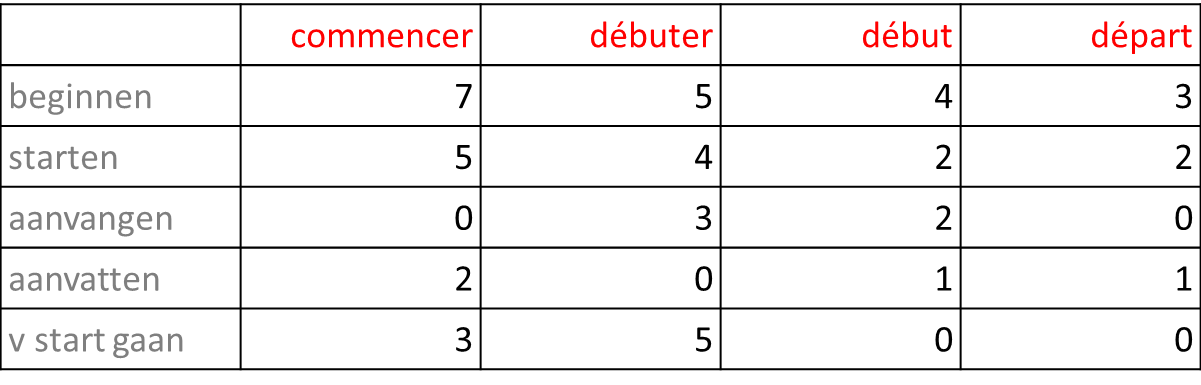
\includegraphics[height=.3\textheight]{figures/Vandevoorde2-img15.png}
\end{table}

The initial map has as many dimensions as there are columns in the data matrix (\figref{fig:key:16}).

\begin{figure}
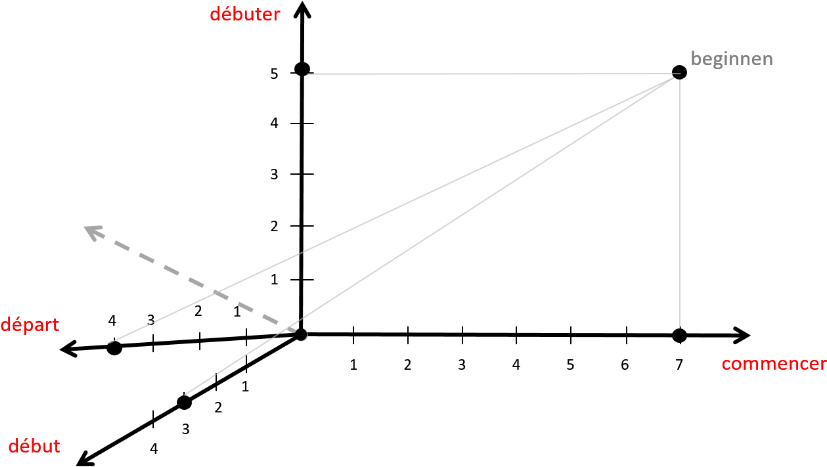
\includegraphics[height=.3\textheight]{figures/Vandevoorde2-img16.png}
\caption{Spatial map with n dimensions for beginnen \label{fig:key:16}}
\end{figure}

Now, in order to be able to visually present the specific geographic position of each of the Dutch lexemes in the rows, their position in the n-dimensional space is reduced to a two-dimensional space. All five Dutch lexemes can be then represented as points in this space (\figref{fig:key:17}):

\begin{figure}
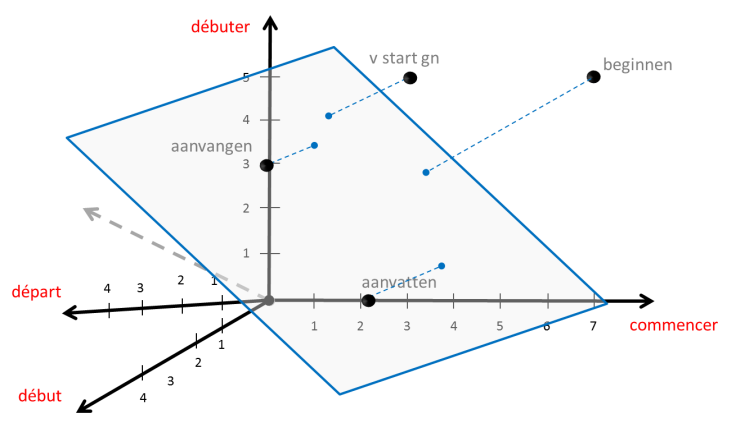
\includegraphics[height=.3\textheight]{figures/Vandevoorde2-img17.png}
\caption{Reduction to a two dimensional space for all rows \label{fig:key:17}}
\end{figure}

Next, the best fitting two-dimensional space is computed (\figref{fig:key:18}). Because this two-dimensional map captures the original high-dimensional data cloud as much as possible, it is true that “the larger the distance between two rows, the further these two rows should be apart in the map for rows” \citep[129]{baayen_analyzing_2008}. Consequently, the positions of the lexemes and the distances between the plotted lexemes represent the similarities and differences between the lexemes. The same computation is repeated for the columns of the frequency table and the simultaneous representation of the row map and the column map results in a so-called bi-plot (representing the scatterplot of the row map and the scatterplot of the column map simultaneously) (\figref{fig:key:18}):

\begin{figure}
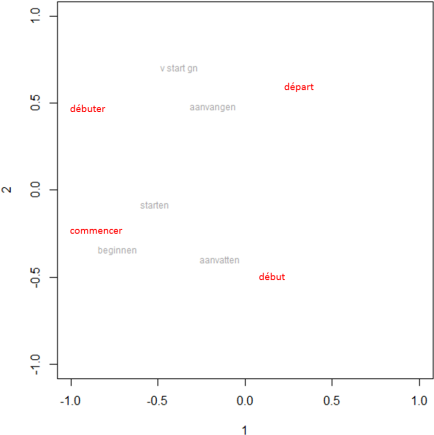
\includegraphics[height=.3\textheight]{figures/Vandevoorde2-img18.png}
\caption{\label{fig:key:18}  Bi-plot for fictitious data matrix in \tabref{tab:key:12}}
\end{figure}

When CA is applied to the data sets gathered for this study, a first visualization via CA of the SourceDutch field of \textit{beginnen} looks is obtained (\figref{fig:key:19}):


\begin{figure}
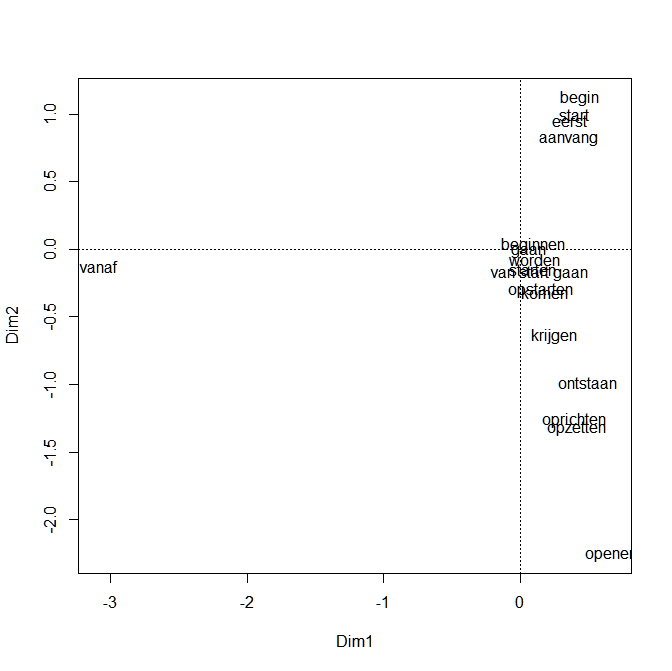
\includegraphics[height=.3\textheight]{figures/Vandevoorde2-img19.png}
\caption{\label{fig:key:19}  First Correspondence Analysis of SourceDutch field for \textit{beginnen}}
\end{figure}

What is immediately striking is the outlying position of \textit{vanaf}. Although the selection of lexemes has been done through a carefully developed technique, described in the previous sections, it is decided to exclude \textit{vanaf} from all data sets. Looking back at the frequency tables (the second T-images of beginnen\textsubscript{ENG} and beginnen\textsubscript{FR}, see appendices E and F) for SourceDutch, it is indeed striking that \textit{vanaf} has an “unusual profile” \citep[92]{greenacre_correspondence_2007}: \textit{vanaf} is related to a single French target lexeme, i.e. \textit{à} \textit{partir} \textit{de}. In the second T-image of beginnen\textsubscript{FR}, we also see that the relative weight of \textit{vanaf} is rather high (0.1505792; representing 15 \% of the total number of observations) and contributing to a 0.1953608 – over 19\% – rise of the total inertia\footnote{“1. The (total) inertia of a table quantifies how much variation is present in the set of row profiles or in the set of column profiles” […] 3. CA is performed with the objective of accounting for a maximum amount of inertia along the first axis. The second axis accounts for a maximum of the remaining inertia, and so on. […]” \citep[88]{greenacre_correspondence_2007}.} of the data matrix when compared to the same data matrix without \textit{vanaf}. The conclusion is that the variation of the first dimension is solely accounted for by \textit{vanaf}. \citet[92]{greenacre_correspondence_2007} indeed warns for the fact that outliers can “start dominate a map so much that the more interesting contrasts between the more frequently occurring categories are completely masked”. The data points in the plot without \textit{vanaf} (\figref{fig:key:26}) are indeed more spread out in the two-dimensional space, which will facilitate the interpretation. Based on the above, \textit{vanaf} is removed from all data sets.

Before I further analyze a visualization via CA, the degree of representativeness of the plots with respect to the total variation in each of the data sets needs to be assessed. The measure for variation in a frequency table is the inertia \citep{greenacre_correspondence_2007}. The distribution of inertia over the latent dimensions of the CA can be visualized in a so-called scree plot: the bars show how much of the total variation is associated with each dimension. Consequently, the scree plot indicates how many dimensions are needed to reach a threshold, e.g. 80\%. The scree plots for SourceDutch, TransDutch\textsubscript{ENG} and TransDutch\textsubscript{FR}, show that five dimensions are required for SourceDutch (Figures 20 and 21), three dimensions for TransDutch\textsubscript{ENG} (Figures 22 and 23) and four dimensions for TransDutch\textsubscript{FR} (Figures 24 and 25) in order to represent 80\% of the total variation visually. This presents a practical problem, however, as 4 or 5 dimensional plots are not easily visualized. Although a visualization via CA for SourceDutch only represents around 40\% of the inertia, the visualization in \figref{fig:key:26} is presented as a first, exploratory analysis of the field of SourceDutch.

\begin{figure}
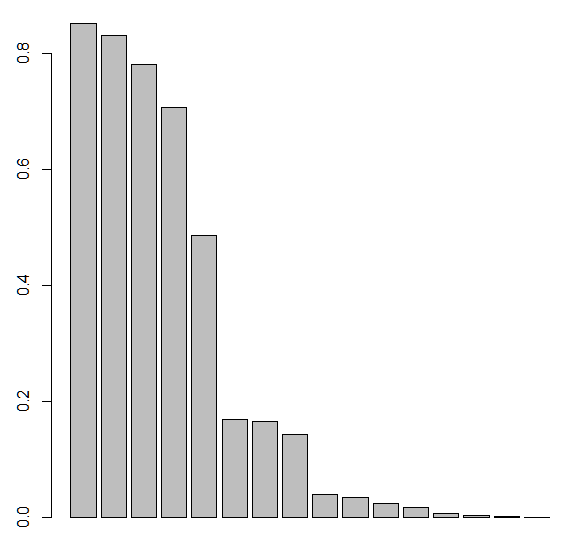
\includegraphics[height=.3\textheight]{figures/Vandevoorde2-img20.png}
\caption{\label{fig:key:20}  Scree plot for SourceDutch}
\end{figure}

\begin{figure}
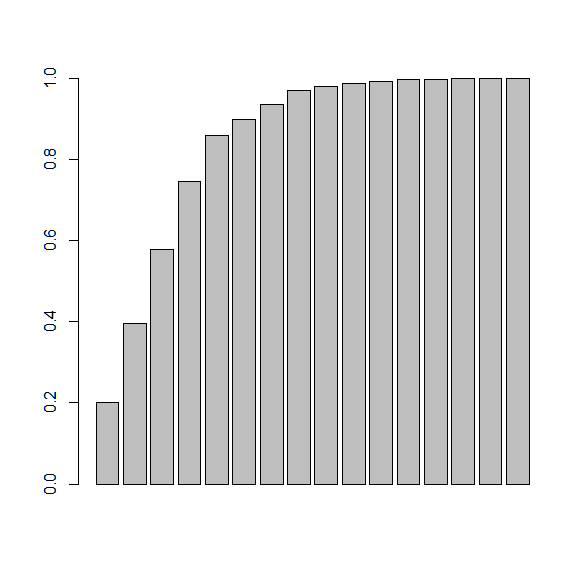
\includegraphics[height=.3\textheight]{figures/Vandevoorde2-img21.png}
\caption{\label{fig:key:21}  Cumulative scree plot for SourceDutch}
\end{figure}

\begin{figure}
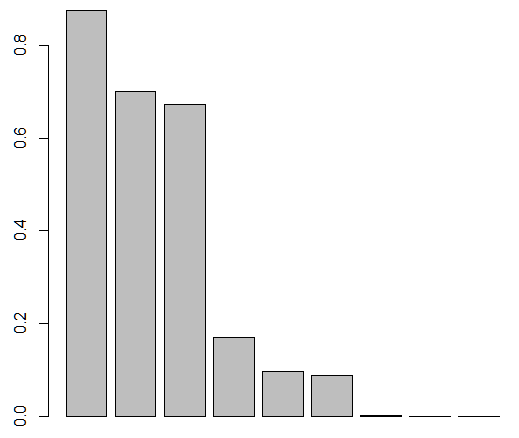
\includegraphics[height=.3\textheight]{figures/Vandevoorde2-img22.png}
\caption{\label{fig:key:22}  Scree plot for TransDutch\textsubscript{ENG}}
\end{figure}

\begin{figure}
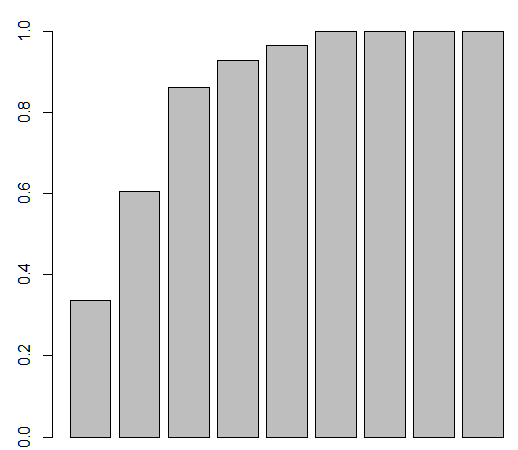
\includegraphics[height=.3\textheight]{figures/Vandevoorde2-img23.png}
\caption{\label{fig:key:23}  Cumulative scree plot TransDutch\textsubscript{ENG}}
\end{figure}

\begin{figure}
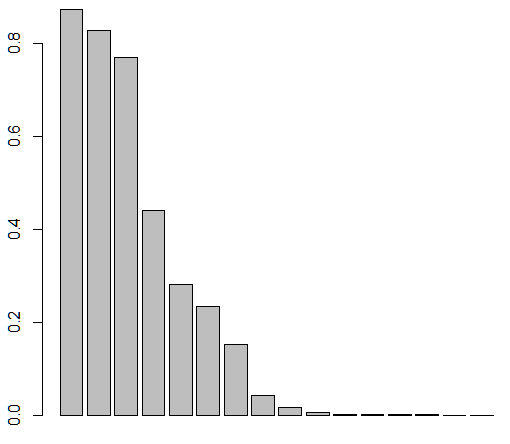
\includegraphics[height=.3\textheight]{figures/Vandevoorde2-img24.png}
\caption{\label{fig:key:24}  Scree plot for TransDutch\textsubscript{FR}}
\end{figure}

\begin{figure}
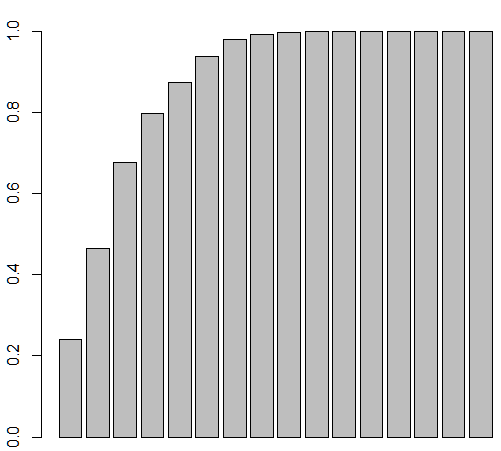
\includegraphics[height=.3\textheight]{figures/Vandevoorde2-img25.png}
\caption{\label{fig:key:25}  Cumulative scree plot for TransDutch\textsubscript{FR}}
\end{figure} 

\begin{figure}
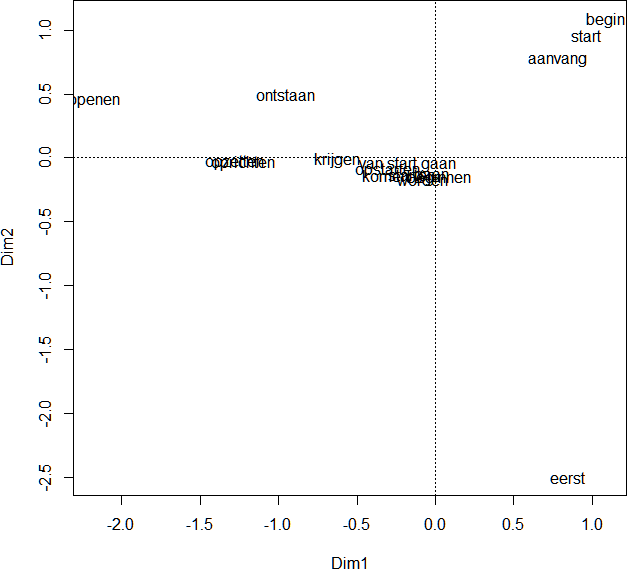
\includegraphics[height=.3\textheight]{figures/Vandevoorde2-img26.png}
\caption{\label{fig:key:26} Correspondence Analysis of SourceDutch field for \textit{beginnen} without \textit{vanaf}}
\end{figure}

In \figref{fig:key:26}, one large central cluster is observed, situated around the origin (the ‘zero-point’) of the plot which contains, amongst other lexemes, the initial lexeme \textit{beginnen}. This central cluster is considered as the prototypical center, consisting of lexemes with the basic meaning of the inchoative category, viz. “start of a general process”. In the upper right corner, a second cluster contains \textit{aanvang} [commencement], \textit{start} [start] and \textit{begin} [beginning]; all three lexemes are nouns, where \textit{start} and \textit{begin} are the nominal derivatives of \textit{beginnen} and \textit{starten} (which belong to the cluster considered as the prototypical center). The third lexeme \textit{aanvang} then, is the more formal\footnote{In order to underpin the assertions presented with respect to the pragmatics or semantics of a given lexeme, I rely on information retrieved in the lexical database Cornetto \citep{spyns_cornetto:_2013}.} counterpart of \textit{begin} and \textit{start}. In the lower right corner, \textit{eerst} [firstly] holds a somewhat outlying position. This outlying position can be explained by the fact that the translations which determine its position (\textit{d’abord} and \textit{firstly}) are almost exclusively used as translations of \textit{eerst}. \textit{Oprichten} [to establish] and \textit{opzetten} [to set up] are furthermore clustering together. In the lexical database Cornetto \citep{vossen_cornetto_2008, spyns_cornetto:_2013}, \textit{oprichten} is defined as \textit{opzetten} and both verbs are indicated to refer to inchoative situations involving a project, a business, a company, etc. In other words, the CA confirms the strong relation between the two lexemes. Finally, \textit{ontstaan} [to come into being] and \textit{openen} [to open] occupy a somewhat unclear position between the center and periphery of the graph. On the basis of the CA, three different clusters can be discerned: one central cluster (considered as the one with the most prototypical expressions of inchoativity); one cluster containing the nominal derivatives of \textit{beginnen} and \textit{starten} plus \textit{aanvang}, a small third cluster with the near-synonymous verbs \textit{oprichten} and \textit{opzetten}. It is not entirely clear whether \textit{ontstaan} and \textit{openen} could be considered as one cluster, or whether they should be considered as two separate, singleton clusters.

Due to the subtlety of the semantic field, the delimitation of clearly distinct clusters can appear difficult. A drawback of CA moreover is that it does not allow to further analyze the central cluster: the visualization only suggests that the lexemes within this cluster are closely related, but the exact relations remain unclear.

Conclusively, the following observations can be made on the basis of this preliminary CA. Firstly, an outlying data point which was distorting the overall interpretation of the data (\textit{vanaf}) was detected and removed. Secondly, the scree plots for SourceDutch, TransDutch\textsubscript{ENG} and TransDutch\textsubscript{FR} showed that for these data sets, more than 2 dimensions are required to accurately represent the distribution of the inertia over the latent dimensions of the CA. This represents a practical problem with respect to visualization. Thirdly, a first exploration of the SourceDutch field on the basis of the CA allowed to formulate some preliminary insights into the semantic field. However, the delimitation of clearly distinct clusters appeared difficult and the exact relations between the lexemes in the central cluster could not further be examined. It was therefore decided to use Hierarchical cluster Analysis for the visualization of the semantic fields of SourceDutch, TransDutch\textsubscript{ENG} and TransDutch\textsubscript{FR}. The HCA will be carried out on the output of a CA, a procedure which will be further explained in the next section.

\subsection{Hierarchical Cluster Analysis}
\label{sec:3.7.2}  
Hierarchical Cluster Analysis (HCA) can be defined as “a collection of different algorithms that puts objects into clusters according to well-defined similarity rules” and is “mostly used when we do not have any a priori hypotheses” \citep[406]{glynn_cluster_2014}. In this section, I will first describe which type of cluster analysis seems the best choice for this study. In addition, as every cluster analysis is crucially dependent on both a particular similarity measure and clustering algorithm, I will elaborate on these measures in \sectref{sec:3.7.2.1} and \sectref{sec:3.7.2.2} respectively. Next, I will explain the procedure for determining the number of clusters for which I will rely on the R package pvclust \citep{suzuki_pvclust:_2006} (\sectref{sec:3.7.2.3}). Finally, I propose a validation of the combined choice of a particular similarity measure and clustering algorithm and of the number of clusters in the cluster solution (\sectref{sec:3.7.3.4}\todo{No such section})\footnote{Exhaustive overviews of the existing clustering techniques can be found in \citet[495-523]{manning_foundations_1999}, \citet[138-148]{baayen_analyzing_2008},  \citet[71-110]{everitt_cluster_2011}, \citet[336-349]{gries_statistics_2013} and \citet{glynn_cluster_2014}.}.

Just as semantic spaces are customary in computational semantics, in (cognitive) linguistics, “[c]luster analyses have been used to determine the similarity of intraword senses or the degree of granularity exhibited by polysemous word senses (cf. \citealt{steinberg_empirical_1971,sandra_network_1995,putz_prepositional_1996})” (\todo{REF unclear}\citealt[81]{Gries2006b}). The method has also been extensively used by Gries and Divjak (see for example \citealt{divjak_ways_2006, divjak_structuring_2010,glynn_cluster_2014,divjak_ways_2006, evans_behavioral_2009,Gries2006,evans_behavioral_2009,gries_behavioral_2010,deshors_case_2014})\todo{REF unclear}. The reasons for HCA’s popularity are summarized by Divjak:

\begin{quote}
Cluster analysis is one of the basic exploratory techniques that are often applied in analyzing large data sets. This statistical method helps organize observed data into meaningful structures: it finds similarities between elements and groups similar elements together. These groupings, in turn, assist in understanding relationships that might exist among these elements. In other words: cluster analysis finds the most optimal solution and organizes an enormous number of data in substructures that facilitate comparison of the (elements in the) structures to each other (Divjak, 2010, 129-130).\todo[inline]{REF unclear}
\end{quote}

HCA is not a single technique, but covers “a family of techniques for clustering data and displaying them in a tree-like format” \citep[138]{baayen_analyzing_2008}. In Statistical NLP, HCA has two main uses: exploratory data analysis on the one hand and generalization on the other hand \citep[497]{manning_foundations_1999}. The tree-like format in which the result of a clustering algorithm can be visually represented is called a dendrogram:

\begin{quote}
a branching diagram where the apparent similarity between nodes at the bottom is shown by the height of the connection which joins them. Each node in the tree represents a cluster that was created by merging two child nodes. [...] The “height” of the node corresponds to the decreasing similarity of the two clusters that are being merged \citep[495]{manning_foundations_1999}.
\end{quote}

In order to maintain terminological clarity, I propose to use the following terminology (visualized in \figref{fig:key:27}), which is to a large extent based on Everitt et al. (2011, 89). A \textit{node} can refer to either an \textit{internal} \textit{node}, a \textit{sub-node} (an internal node within one delimited cluster) or a \textit{terminal} \textit{node} (also called a \textit{leave}). The \textit{heights} of the \textit{edges} can be read off from the dendrogram. The line perpendicular to the edges in the tree is called the \textit{root}. Finally, I will call the names printed at the extremities of every terminal node \textit{lexemes} or \textit{lexical} \textit{items} (which is an immediate adaptation of the terminology to the type of data in this book) instead of the term \textit{label} proposed by \citet{everitt_cluster_2011}. 

\begin{figure}
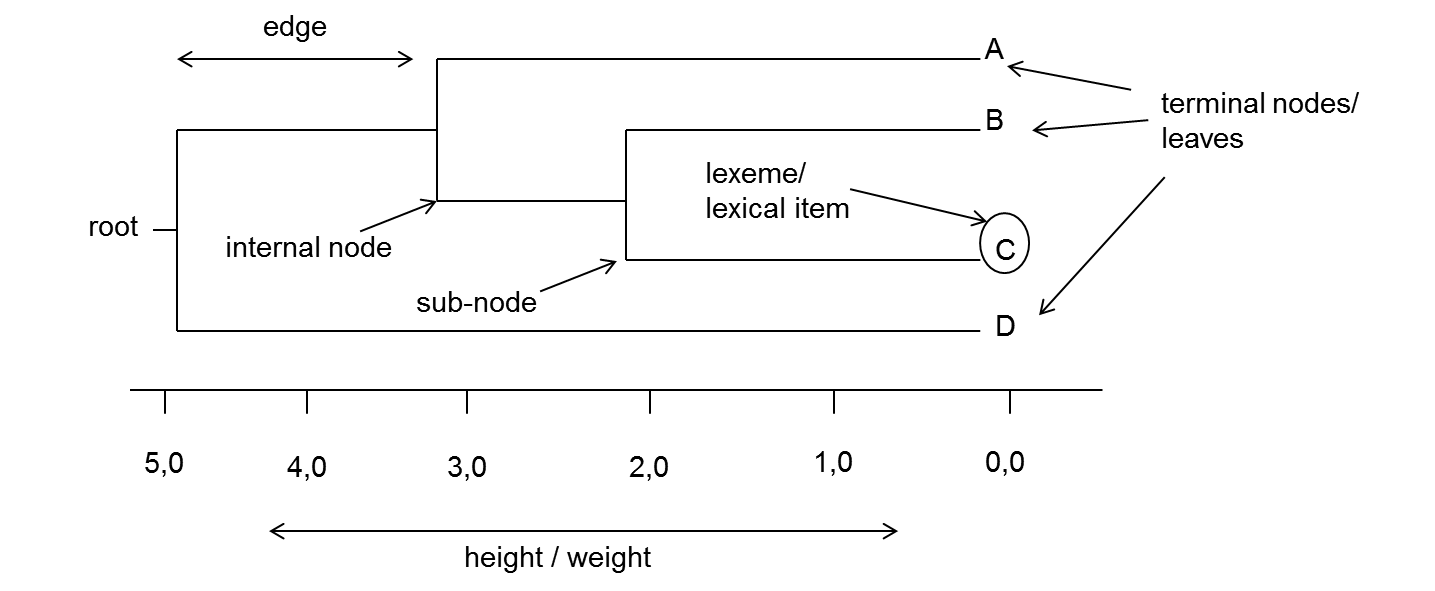
\includegraphics[height=.3\textheight]{figures/Vandevoorde2-img27.png}
\caption{\label{fig:key:27}  Terminological description of a dendrogram (adapted from \citealt[89]{everitt_cluster_2011})}
\end{figure}

HCA comes in two flavors: the \textit{tree} can be constructed either top-down or bottom-up. The first method is called divisive clustering where “one starts with all the objects and divides them into groups so as to maximize within-group similarity” \citep[501]{manning_foundations_1999}. The second method is called agglomerative clustering which works “by starting with the individual objects and grouping the most similar ones (Ibid., 500-501)\todo{Fix ref}”. Divisive clustering – also called partitioning – is known to have difficulties in finding “optimal divisions for smaller clusters” and appears to be better at finding a few large clusters \citep[138]{baayen_analyzing_2008}. This can be verified by the visualized result in \figref{fig:key:28}, which shows a so-called \textit{chaining} \textit{effect} when applying divisive clustering for TransDutch\textsubscript{ENG}. This means that the cluster tree displays “a chain of large similarities without taking into account the global context” \citep[504]{manning_foundations_1999}. As Manning and Schütze argue, cluster analysis is normally based on “the assumption that ‘tight’ clusters are better than ‘straggly’ clusters”, and that this in turn “reflects an intuition that a cluster is a group of objects centered around a central point, and so compact clusters are to be preferred” (p.506). In particular, this corresponds to “a model like the Gaussian distribution”(Ibid.)\todo{Fix ref}. Although Manning and Schütze stress that this is “only one possible underlying model of what a good cluster is”, and that a good clustering should rely on prior knowledge or a model of the data, “elongated clusters” due to a chaining effect are usually disfavored to sphere-shaped clusters (Ibid.)\todo{Fix ref}. Because the dendrograms will be interpreted as semantic fields of \textit{beginnen}, organized in a prototype-based manner – with the different clusters representing the meaning differentiations of the lexeme under study – I will prefer a clustering which indeed reflects my intuition that the clusters are centered around a central point and avoids large, elongated clusters caused by a chaining effect.

In summary, I follow \citet[92]{everitt_cluster_2011} who state that the chaining effect is a symptom of distortion through “space contraction” where “dissimilar objects are drawn into the same cluster” \citep[92]{everitt_cluster_2011}. \citet[92]{everitt_cluster_2011} point out that a second type of distortion exists, called ‘space-dilation’ which takes place “where the process of fusing clusters tends to draw clusters together” (Ibid.)\todo{Fix ref}. \figref{fig:key:29} illustrates such a space-dilation effect, of which I will also be wary.

\begin{figure}%%[Warning: Draw object ignored]
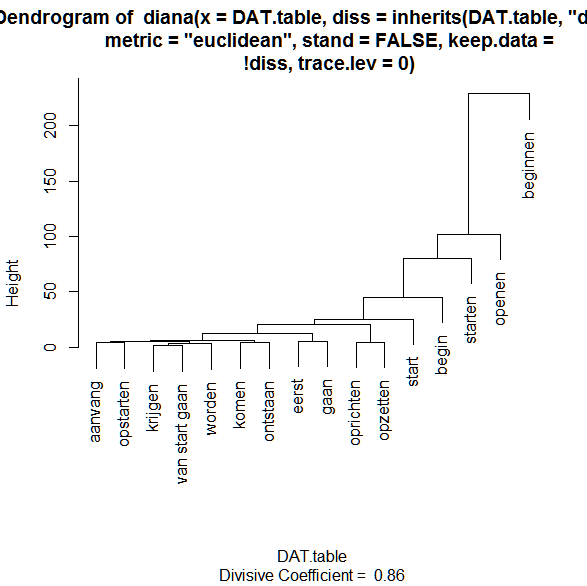
\includegraphics[height=.3\textheight]{figures/Vandevoorde2-img28.png}
Chaining effect
\caption{\label{fig:key:28}Divise clustering of the field of TransDutch\textsubscript{ENG}, displaying chaining effect}
\end{figure}

\begin{figure}%%[Warning: Draw object ignored]
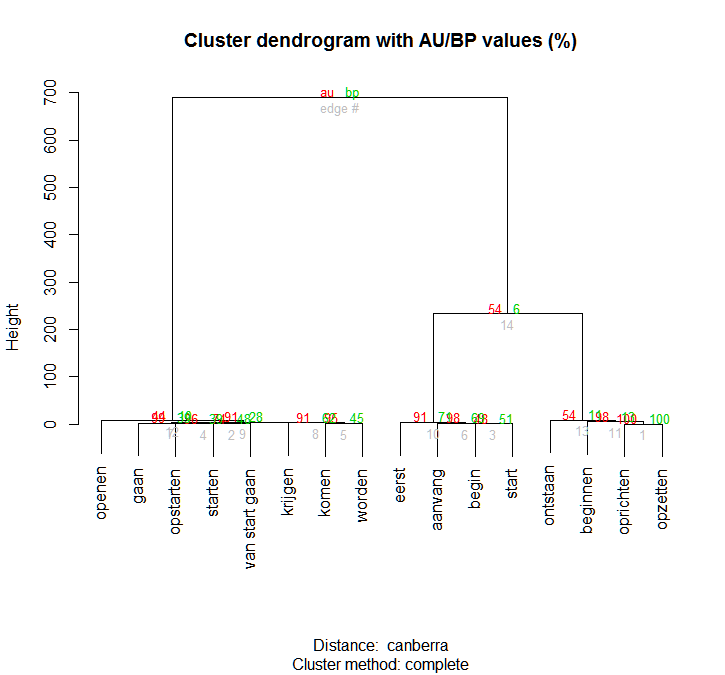
\includegraphics[height=.3\textheight]{figures/Vandevoorde2-img29.png}
Space dilation
\caption{\label{fig:key:29} Agglomerative clustering of the field of SourceDutch, displaying space-dilation}
\end{figure}

As a consequence, the data will be further explored with hierarchical agglomerative clustering (HAC). In addition, the HAC will be carried out on the resultant coordinates of the CA. I thereby follow (\citet[335]{cuadras_correspondence_1993} who suggest “to complement it [a CA] with a classification”, as this “can supply elements of information that could have been hidden by the projection onto a low dimensional subspace” (see also \citealt[28]{ciampi_correspondence_2005}). A HAC performed on the output of a CA has obvious advantages as CA involves dimension reduction: noisy dimensions are omitted and only informative dimensions are retained. By selecting only the informative dimensions of the CA as input for the HAC, such an analysis is likely to be better interpretable than a HAC on raw data. In other words, this procedure ‘combines the best of two worlds’: CA allows to detect informative dimensions of variation to the detriment of noise, and with HAC meaningful structure(s) in the data cloud can be discerned.

Since I will use the output of the CA as input for a HAC, I use the fast\_sca() function of the svs{}-package to obtain the coordinates (the coordinates can also be obtained by applying the ca() function in R). The svs{}-function fast\_sca() is especially designed to further use the resultant coordinates of a CA as the input for an additional analysis.

\subsubsection{(Dis)similarity measure}
\label{sec:3.7.2.1}
Clustering algorithms depend crucially on similarity which is understood as “its everyday meaning of how similar entities are” \citep[411]{glynn_cluster_2014}. For numerical variables, similarities are often converted into dissimilarities (or distance). This can be done by subtracting the measure of similarity from 1. In this way, 0 indicates minimum dissimilarity and 1 maximum dissimilarity \citep[415-416]{glynn_cluster_2014}. There is a wide variety of distance measures, but I will limit the comparison to two measures which are customarily used in linguistics: the Euclidean distance and the Canberra distance, the latter is known to handle sparse data and zero-occurrences best \citep[132]{divjak_structuring_2010}. Based on the outcome of the comparison (which will be presented in \sectref{sec:3.7.2.4}), Euclidean will be chosen as the distance measure for the analyses in this book.

\subsubsection{Clustering Algorithm}
\label{sec:3.7.2.2}  
Next to an appropriate distance measure, a clustering algorithm also depends on a so-called amalgamation rule. This determines “which clusters are merged in each step in bottom-up clustering” \citep[503]{manning_foundations_1999}. In fact, the amalgamation rule is the defining feature of the various agglomerative cluster algorithms as it specifies in which way the proximity between two clusters will be computed; “the definition of cluster proximity that differentiates the various agglomerative hierarchical techniques” \citep[517]{tan_introduction_2006}. The most important cluster algorithms are the following:

Single-link clustering (also called nearest neighbor or single linkage algorithm) considers the similarity between two clusters as “the similarity of the two closest objects in the clusters” \citep[503]{manning_foundations_1999}. This algorithm is known to produce locally coherent clusters, but with a bad global quality \citep[503]{manning_foundations_1999}; the clusters moreover tend to show a chaining effect (\citep[504]{manning_foundations_1999}.

Complete-link clustering (also called furthest neighbor or complete linkage algorithm) “focuses on global cluster quality [...]. The similarity of two clusters is the similarity of their two most dissimilar members” \citep[505]{manning_foundations_1999}. This algorithm is known to avoid chaining effect, which is preferable in NLP applications \citep[506]{manning_foundations_1999}.

Group-average agglomerative clustering (or average linkage) is a compromise between the previous two algorithms, which uses the average similarity as a criterion to merge items into clusters \citep[507]{manning_foundations_1999}. It can be considered as an alternative to complete-link clustering and it is also known to avoid chaining effect.

Ward’s Minimum Variance Method is a somewhat different clustering algorithm as it “allows two clusters to merge if the increase in sum of squared distances\footnote{The sum of squares is a measure of variation, calculated by summing the squares of the differences from the mean.} of the members of the new cluster from their mean is smaller than for any other possible merger between two clusters. Use of squared distances penalizes spread out clusters and so results in compact clusters without being as restrictive as complete linkage” \citep[426]{glynn_cluster_2014}. Because of its tendency to find spherical clusters, Ward’s Method is “a frequently recommended strategy that yields small clusters” \citep[133]{divjak_structuring_2010}.

The above mentioned algorithms can themselves be grouped according to the different views on clusters they reflect. Depending on the goals one defines, different types of clusters can be found useful. Tan et al. (2006, 493–95) distinguish five types of cluster solutions: well-separated clusters (each object in a cluster is closer or more similar to every other object in the cluster than to any object not in the cluster), prototype-based clusters (each object in the cluster is closer or more similar to the prototype that defines the cluster than to the prototype of any other cluster), graph-based clusters (nodes are seen as objects; the links represent connections among the objects), density-based clusters (a cluster is seen as a dense region of objects surrounded by a region of low density) and shared-property clusters (also called conceptual clusters, where a cluster is a set of objects that share some property). Single linkage, complete linkage and average linkage algorithms suit a graph-based view of clusters; Ward’s Method, on the other hand, is the more natural choice when one adheres a prototype-based view on clusters, since it “assumes that a cluster is represented by its centroid [...]” \citep[517]{tan_introduction_2006}.

Which cluster algorithm is the ‘right’ one for this purpose, is not a trivial question, as different algorithms yield different dendrograms. \citet[132]{divjak_structuring_2010}, following \citet[35]{speece_cluster_1994} emphasizes to choose the algorithms whose “ “side-effects” of the mathematical properties [...] fit the phenomenon under investigation, and, consequently, yield easily interpretable results”. 

The single-linkage method is discarded because of its tendency to produce chaining effect. For the other cluster algorithms, however, it is not so clear which method is preferable. From the previous descriptions, Ward’s Method seems to suit my needs best: it can yield small clusters – as a “side-effect of its mathematical properties” – and it reflects a prototype-based view on clusters. The choice of Ward’s Minimum Variance method is also what results from the comparison with the complete and average linkage methods in \sectref{sec:3.7.2.4}. HAC is carried out on the output of the CA with the function pvclust() from the package pvclust which relies on the function hclust() (the choice of pvclust will be substantiated in the next section).

\subsubsection{Number of clusters}
\label{sec:3.7.2.3} 
An important issue of HAC concerns the choice of the number of clusters, i.e., the ‘optimal cluster solution’. This is obtained by ‘cutting’ the tree at a particular height into n clusters. The height of the tree cut must be chosen carefully, as the resulting clusters will be considered as meaningful and informative in the subsequent interpretation. There is, however, no straightforward procedure to determine the ‘best cut’. As a rule of thumb, several scholars suggest that looking at the length of the vertical lines in the dendrogram is indicative for the ‘optimal cluster solution’. Gries mentions that “large vertical lines indicate more autonomous subclusters”(\citeyear[338]{gries_statistics_2013}). Similarly, (\citet[430]{glynn_cluster_2014} propose to “look at the height bar and choose a place where the cluster structure remains stable for a long distance”. Finally, \citet[95]{everitt_cluster_2011} assert that “large changes in fusion levels are taken to indicate the best cut”. Divjak \& Fieller admit that such suggestions are not exactly what we would call “frivolous” (\citeyear[430]{glynn_cluster_2014}). To somewhat remedy this, they mention three criteria which can help to make a decision on the cut height. A ‘good’ cut height should give (i) enough clusters in the solution for it to be meaningful (i.e. an acceptable size); (ii) an immediately intuited meaning for each/most of the clusters and (iii) criterion validity (the expected level of association between rows and columns should be acceptably reflected). (\citet[432-433]{glynn_cluster_2014} furthermore propose two ways to investigate the robustness of a cluster solution: the computation of the average silhouette width and the use of bootstrap validation.

The optimal cluster solution will be determined by means of a bootstrap validation technique (I will use average silhouette width as a cluster validation technique, as explained further on in this section). Bootstrapping entails that the data are resampled (with replacement) a high number of times (i.e. usually 3000) in order to see how many times the same points are clustered together again. On the basis of these replications a p-value is computed for each node of the dendogram (i.e. the place where two branches join). As a consequence, the bootstrap p-values represent a measure of quality for each node. This bootstrap validation will be done with the R package pvclust \citep{suzuki_pvclust:_2006}. As a matter of fact, the pvclust package provides both an “approximately unbiased p-value” and a “bootstrap probability” (the use of the former is recommended by Suzuki \& Shimodaira). In addition, the package has the function pvrect which can be used to cut the dendrogram at the nodes above a certain confidence level, e.g. 95\%. This has a clear advantage over tree cuts at a fixed height. Fixed-height cuts are common in HAC but not indispensable. \citeauthor{everitt_cluster_2011} warn that fixed-height cut methods require pre-established cut heights and minimum cluster size which can possibly be influenced by a priori expectations (\citeyear[95]{everitt_cluster_2011}).

If possible, I will always cut the tree at the highest significant node attaining a confidence level of 95\%. However, this procedure runs the risk of excluding many-cluster-solutions: e.g. if the two highest nodes in a tree are significant, pvrect would choose a two-cluster-solution. Such solutions with very few clusters might be less interpretable than. As a consequence, I propose a compromise of cutting a dendrogram at a confidence level and cutting it at a fixed height: the cutoff point will be chosen so that for each cluster in the solution, the highest node within each cluster is significant (the Approximately Unbiased p\textsuperscript{{}-}value should be ${\geq}$ 0.95; an exception is made for singleton clusters). In this way the validated cluster solution meets the first two criteria mentioned by Divjak \& Fieller for good cut height (acceptable cluster size and meaningful clusters).

\subsubsubsection{Validation of the number of clusters}
In the first part of this section bootstrap p-values were proposed to determine the number of clusters. That procedure is now complemented with two techniques for testing the validity of a cluster solution. The first validation consists in the computation of the average silhouette widths proposed by \citet{kaufman_finding_1990}, the second one is a (non-hierarchical) K-means clustering.

\citet{kaufman_finding_1990} propose to calculate the silhouette width for each object in a cluster solution and summarize this information in a silhouette plot. For each object i, one can “compare i’s separation from its cluster against the heterogeneity of the cluster” \citep[138]{everitt_cluster_2011}. The silhouette width has a value situated between -1 and 1. Values close to 1 imply that “the heterogeneity of object i’s cluster is much smaller than its separation and object i is taken as ‘well classified’” (Everitt et al., Ibid.)\todo{Fix ref}; values close to -1 imply misclassification and values around 0 suggest that the classification is unclear (Ibid.)\todo{Fix ref}. Finally, the average silhouette width – the average of all silhouette widths of a set of data – can be used to validate the chosen cluster solution. Kaufman and Rousseeuw point out that an average silhouette width above 0,5 indicates a good classification, whereas values beneath 0.2 betray an unclear classification. In addition, \citet[129]{everitt_cluster_2011} suggest using the average silhouette widths as an instrument for optimizing the number of clusters. The average silhouette width can be calculated using the pam() function of the cluster{}-package.

Although K-means clustering can be run as a separate clustering procedure, I will use it as a validation of the HAC. More specifically, I will compute the centers of the clusters from the HAC and feed those into a K-means clustering. If the partitioning of the lexemes into clusters remains (largely) the same in the K-means clustering, then this can be considered as a validation of the results in the HAC. After calculation of the cluster centroids using centers\_ca() function of svs, K-means clustering can be carried out using the kmeans() function. In contrast to HAC, which does not need a pre-determined number of clusters, non-hierarchical clustering methods such as K-means clustering require a pre-specified number of clusters. More specifically, K-means “defines the clusters by the center of mass of their members” \citep[515]{manning_foundations_1999}, i.e. it takes K points as the centers of the clusters. For the initialization of the K-means algorithm, K points can be randomly chosen from the data to serve as seeds, although predetermined centers can also be supplied (Ibid.)\todo{Fix ref}. The algorithm then consists in iteratively assigning each data point to the cluster to the center of which it is closest (Ibid.)\todo{Fix ref} and subsequently recomputing the centers on the basis of the assignments \citep[515-516]{manning_foundations_1999}. This iterative procedure is carried out until convergence, i.e. until there are no further reassignments.

\subsubsection{Comparison of the chosen procedure with alternative procedures via an assessment of the overall strength of the clustering structure}
\label{sec:3.7.2.4}
The output of a cluster analysis depends on the choice of distance measures and amalgamation rules. In the previous sections, I indicated which distance measure(s) and amalgamation rule(s) are most likely to yield interpretable results for the data of the case study presented in this book. In this section, I will assess various combinations of distance measures (Euclidean and Canberra) and amalgamation rules (Average, Complete, Ward’s) on different spatial maps in order to see which combination works best.

In \sectref{sec:3.7.2}, I substantiated my choice to carry out a HAC on the output of a CA. In addition to this procedure, it is also possible to carry out a HAC directly on the raw data or to compute the distances for the HAC on the output of a Latent Semantic Analysis. LSA is typically considered as a Vector Space Model since “the values of the elements are derived from event frequencies” \citep[144]{turney_frequency_2010} and it is also generally associated with distributional approaches to meaning (Ibid., 141)\todo{Fix ref}. Conceptually, LSA works as follows:

\begin{quote}
LSA projects document frequency vectors into a low dimensional space calculated using the frequencies of word occurrence in each document. The relative distances between these points are interpreted as distances between the topics of the documents \citep[123]{mehler_models_2007}.
\end{quote}

LSA can, by virtue of its symmetry, also be applied to word similarity \citep[123]{mehler_models_2007} and consequently also to translational similarity. In this case, the algorithm of LSA (which is usually applied to a document-term matrix) is applied to a source–target language matrix.

In the subsequent comparison, I will include HAC on the raw data and HAC on the output of a LSA. The various combinations of distance measures (Euclidean and Canberra), amalgamation rules (Complete, Average and Ward’s) and spatial maps (raw data, output of CA, output of LSA) are summarized in \tabref{tab:key:13}. Because of the high number of combinatorial possibilities – 18 in total – I only compare the combinations for the data set SourceDutch. I selected three validation criteria which have in common their ability to assess the overall strength of the clustering structure: agglomerative coefficient, chaining effect and p-values.

Firstly, the agglomerative coefficient for each combination is calculated. This is a standard measure to describe the strength of a clustering structure.

\begin{quote}
The agglomerative coefficient (AC) [is] a measure of the clustering structure of the data set that can range from 0 to 1. An AC close to 1 indicates that a very clear structuring has been found whereas an AC close to 0 indicates that the algorithm has not found a natural structure. This measure is sensitive to sample size, i.e. the value grows with the number of observations \citep[426]{glynn_cluster_2014}.
\end{quote}

Since I am using the same data set for each dendrogram in this comparison, the agglomerative coefficients are comparable. An agglomerative coefficient higher than 0.80 is considered as satisfactory.

Secondly, the output for each combination is visually inspected for presence of chaining effect. For this study, a chaining effect in the cluster structure is disfavored to a sphere-like structure. Hence, the appearance of a chaining effect (as well as of a space-dilation effect) will be considered negative. Because a chaining effect can only be determined on the basis of visual inspection, we introduced four levels of chaining. In \tabref{tab:key:13}, \textit{no} means that no chaining effect was observed, \textit{yes} that a clear chaining effect was observed, \textit{high} means that chaining occurs only in the higher nodes and \textit{low} means that chaining only occurs in the lower nodes. Only those results where a clear chaining effect is observed (\textit{yes}), will be considered negative, no chaining (\textit{no}) will be considered as the most positive outcome.

Finally, the p-values (which were introduced in \sectref{sec:3.7.2.3} to determine the cluster solution) will be used as a third element to assess the overall strength of the clustering structure. To do so, the number of significant nodes (i.e. with a p\textsuperscript{{}-}value of 0.95 or higher) in the dendrogram will be counted. Each of the dendrograms presented in the comparison counts 14 nodes. If ${\geq}$ 7 nodes in the dendrogram are significant, this will be considered as an indication of a strong overall clustering structure. The number in the third column of \tabref{tab:key:13} thus indicates the number of significant p-values (${\geq}$0.95) on a total of 14 nodes.

\begin{table}\caption{Table~13  Combinatory possibilities of the selected distance measures, clustering algorithms and ``spatial maps''. \textsuperscript{†}: (+ high space dilation)\label{tab:key:13}}
\begin{tabular}{llrlr} 
\lsptoprule
&  Procedural combination &  Agglomerative & {Chaining}  & {p-values}\\
&                         &  coefficient   & {effect} \\\midrule
1 & Euclidean, Average          & 0.72 & YES & 10\\
2 & Euclidean, Average, on CA   & 0.74 & YES & 10\\
3 & Euclidean, Average, on LSA  & 0.61 & YES & 8\\
4 & Euclidean, Complete         & 0.73 & YES & 10\\
5 & Euclidean, Complete, on CA  & 0.76 & YES & 9\\
6 & Euclidean, Complete, on LSA & 0.65 & high & 4\\
7 & Euclidean, Ward’s           & 0.78 & YES & 9\\
8 & Euclidean, Ward’s, on CA    & 0.89 & NO & 9\\
9 & Euclidean, Ward’s, on LSA   & 0.72 & NO & 4\\
10 & Canberra, Average          & 0.22 & high & 2\\
11 & Canberra, Average, on CA   & 0.95 & low\textsuperscript{†}  & 6\\
12 & Canberra, Average, on LSA  & 0.82 & NO & 6\\
13 & Canberra, Complete         & 0.27 & NO & 1\\
14 & Canberra, Complete, on CA  & 0.99 & low\textsuperscript{†} & 7\\
15 & Canberra, Complete, on LSA & 0.99 & low\textsuperscript{†} & 9\\
16 & Canberra, Ward’s           & 0.43 & NO & 2\\
17 & Canberra, Ward’s, on CA    & 0.99 & low\textsuperscript{†} & 5\\
18 & Canberra, Ward’s, on LSA   & 0.96 & NO & 3\\
\lspbottomrule
\end{tabular}
\end{table}

\begin{figure}
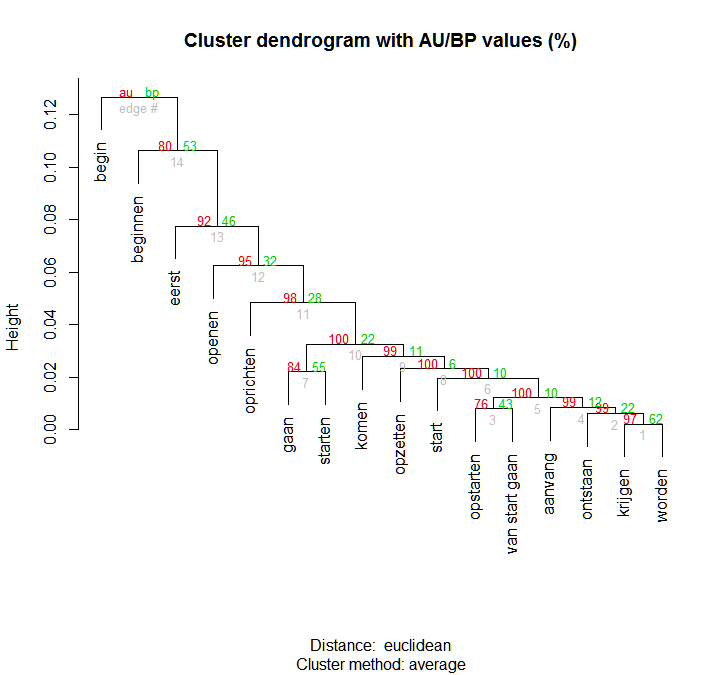
\includegraphics[height=.3\textheight]{figures/Vandevoorde2-img30.png}
\caption{\label{fig:key:30} Euclidean, Average (1)}
\end{figure}

\begin{figure}
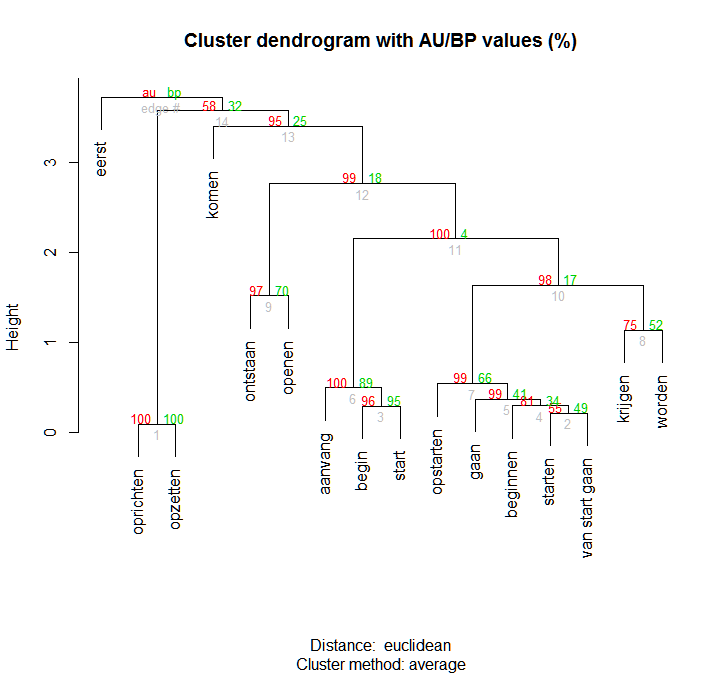
\includegraphics[height=.3\textheight]{figures/Vandevoorde2-img31.png}
\caption{\label{fig:key:31}  Euclidean, Average, on CA (2)}
\end{figure}

\begin{figure}
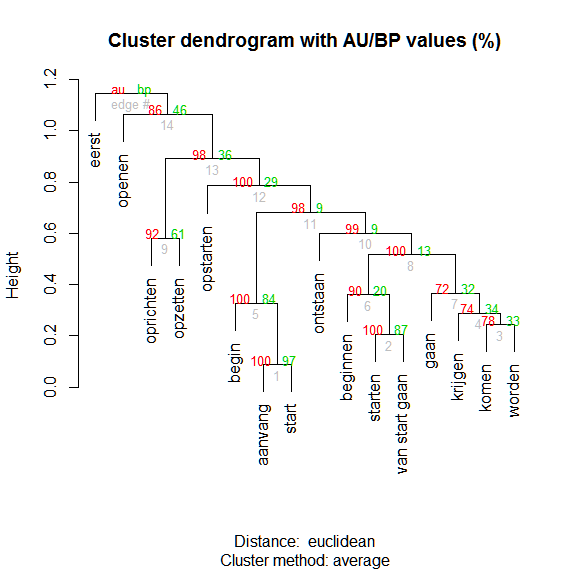
\includegraphics[height=.3\textheight]{figures/Vandevoorde2-img32.png}
\caption{\label{fig:key:32}  Euclidean, Average, on LSA (3)}
\end{figure}

\begin{figure}
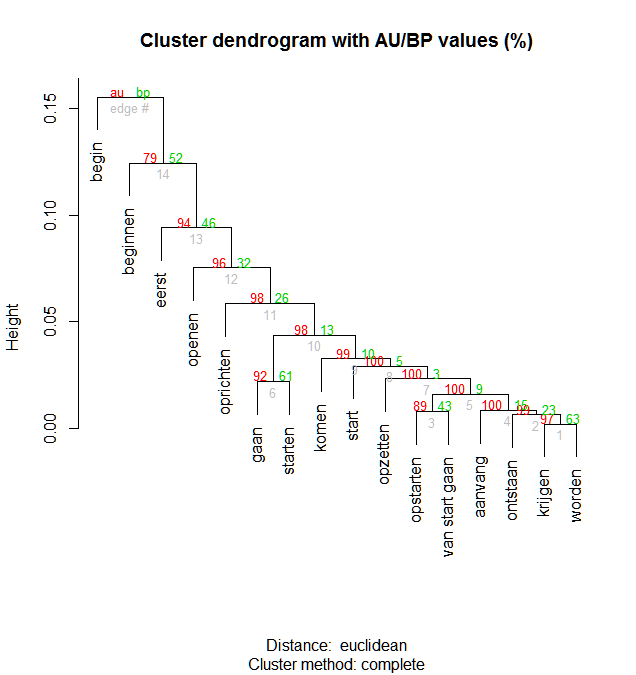
\includegraphics[height=.3\textheight]{figures/Vandevoorde2-img33.png}
\caption{\label{fig:key:33}  Euclidean, Complete (4)}
\end{figure}

\begin{figure}
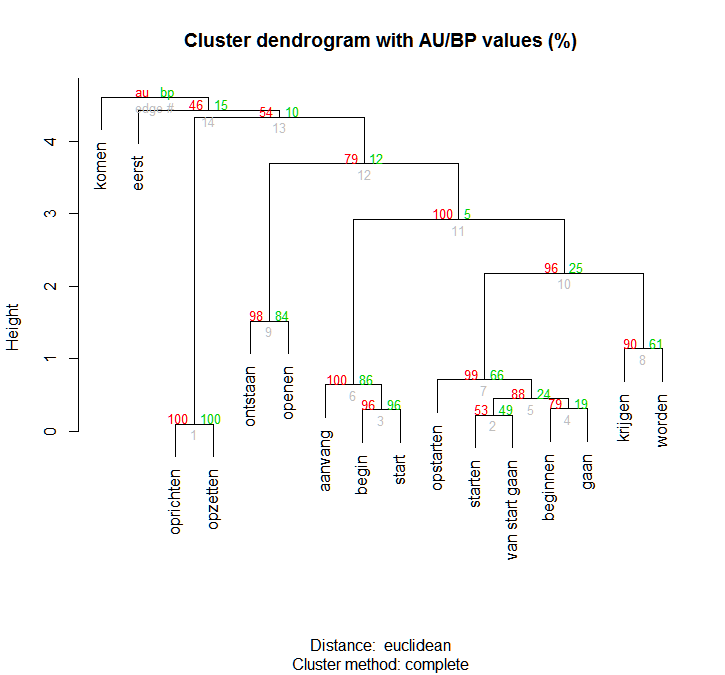
\includegraphics[height=.3\textheight]{figures/Vandevoorde2-img34.png}
\caption{\label{fig:key:34}  Euclidean, Complete, on CA (5)}
\end{figure}

\begin{figure}
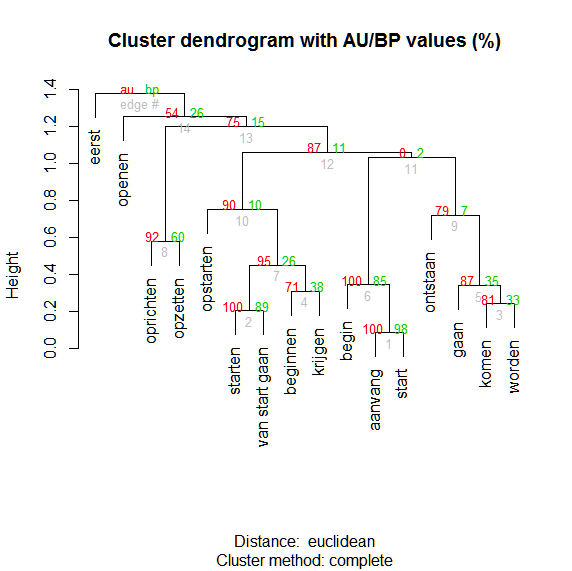
\includegraphics[height=.3\textheight]{figures/Vandevoorde2-img35.png}
\caption{\label{fig:key:35}  Euclidean, Complete, on LSA (6)}
\end{figure}

\begin{figure}
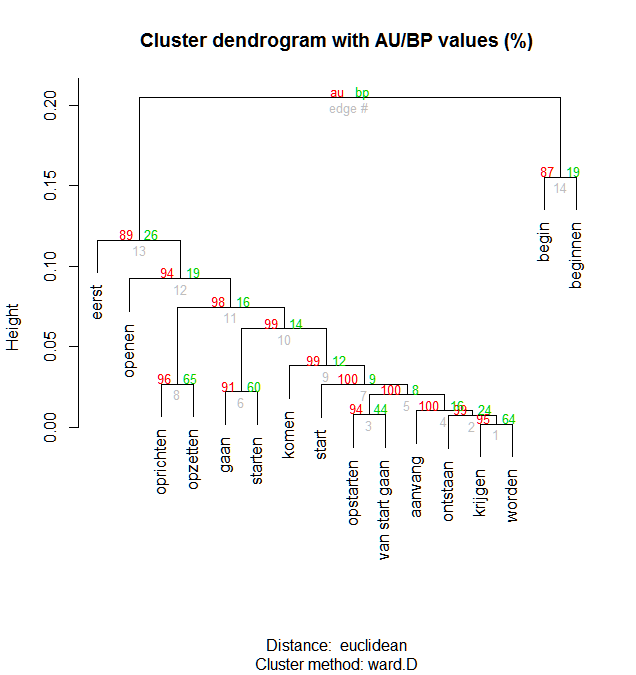
\includegraphics[height=.3\textheight]{figures/Vandevoorde2-img36.png}
\caption{\label{fig:key:36}  Euclidean, Ward’s (7)}
\end{figure}

\begin{figure}
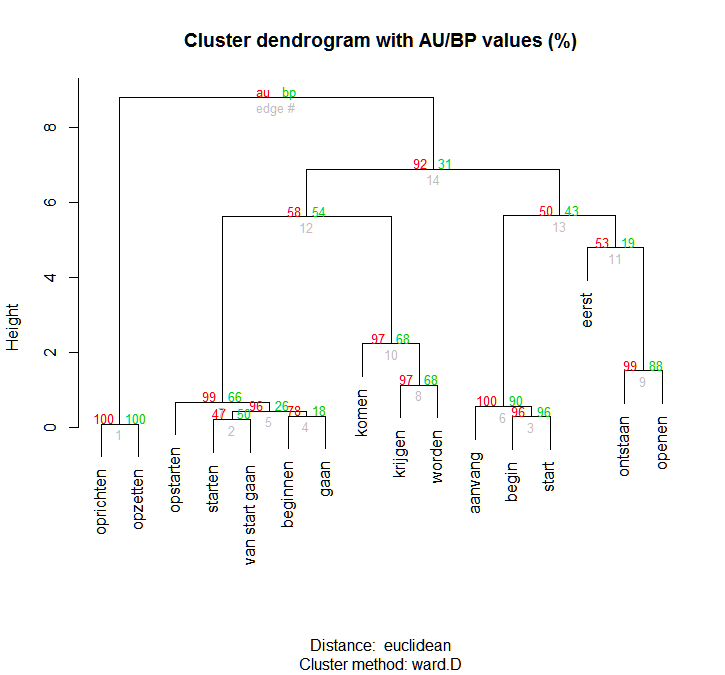
\includegraphics[height=.3\textheight]{figures/Vandevoorde2-img37.png}
\caption{\label{fig:key:37}  Euclidean, Ward’s, on CA (8)}
\end{figure}

\begin{figure}
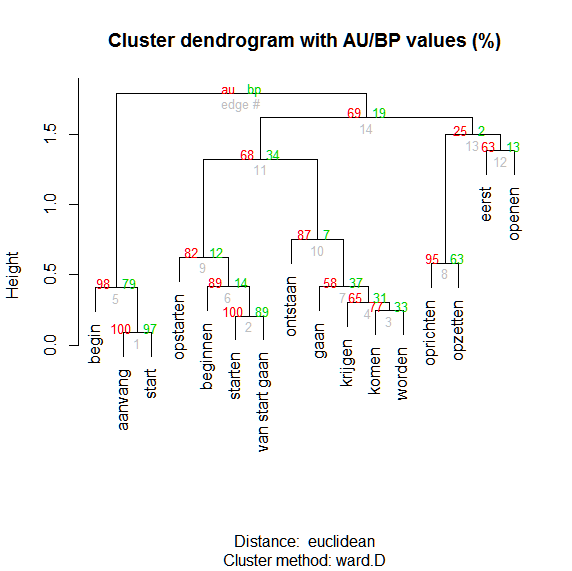
\includegraphics[height=.3\textheight]{figures/Vandevoorde2-img38.png}
\caption{\label{fig:key:38}  Euclidean, Ward’s, on LSA (9)}
\end{figure}

\begin{figure}
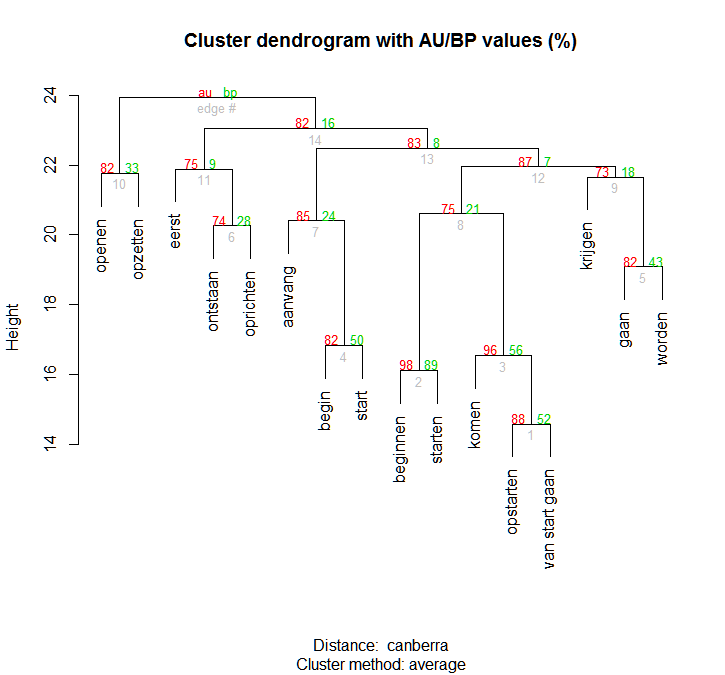
\includegraphics[height=.3\textheight]{figures/Vandevoorde2-img39.png}
\caption{\label{fig:key:39}  Canberra, Average (10)}
\end{figure}

\begin{figure}
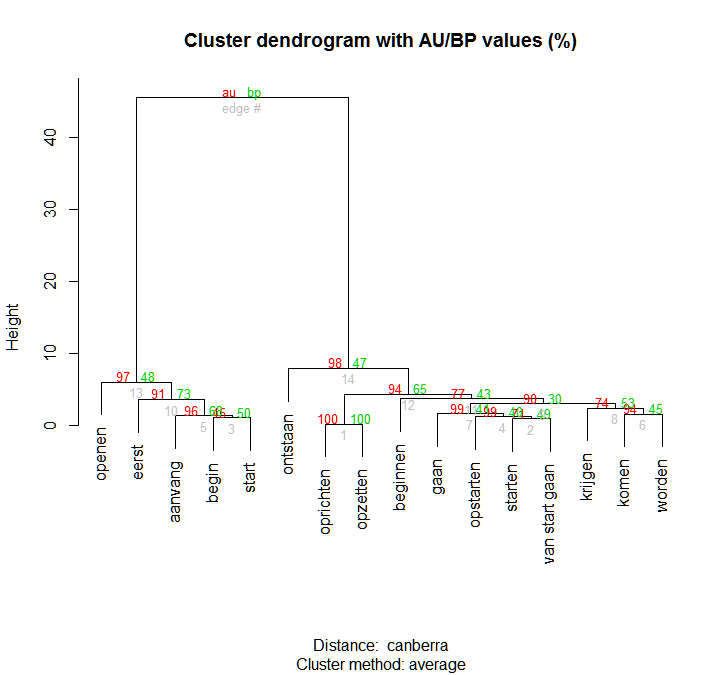
\includegraphics[height=.3\textheight]{figures/Vandevoorde2-img40.png}
\caption{\label{fig:key:40}  Canberra, Average, on CA (11)}
\end{figure}

\begin{figure}
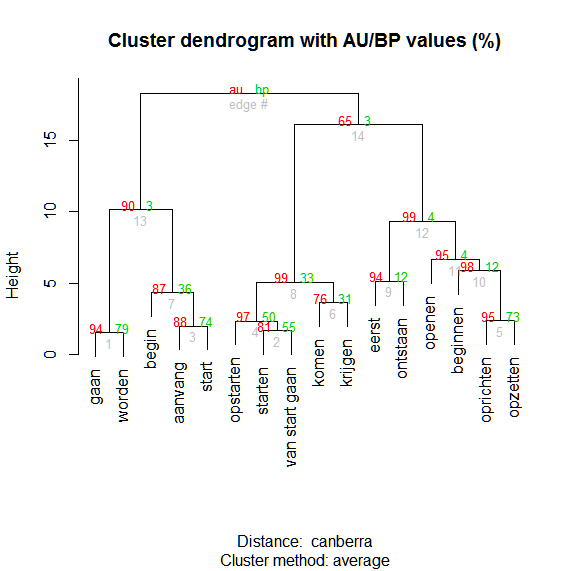
\includegraphics[height=.3\textheight]{figures/Vandevoorde2-img41.png}
\caption{\label{fig:key:41}  Canberra, Average, on LSA (12)}
\end{figure}

\begin{figure}
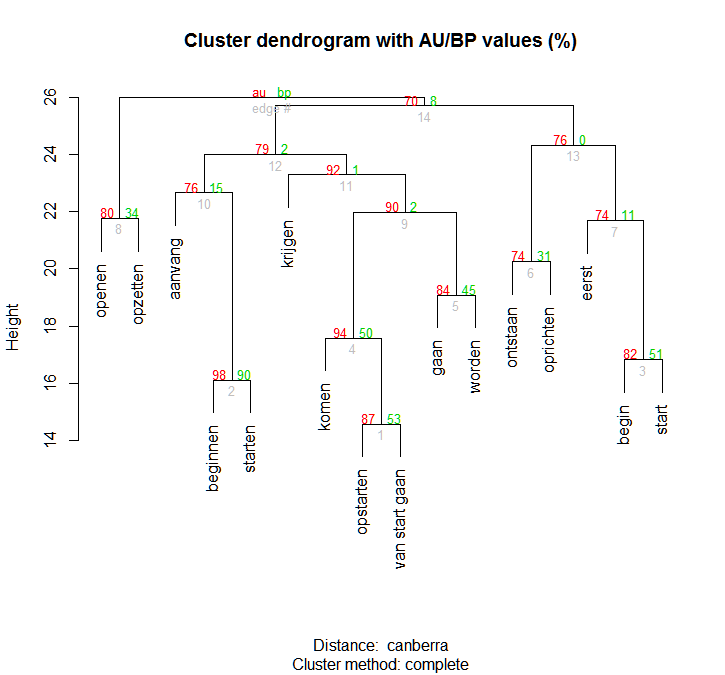
\includegraphics[height=.3\textheight]{figures/Vandevoorde2-img42.png}
\caption{\label{fig:key:42}  Canberra, Complete (13)}
\end{figure}

\begin{figure}
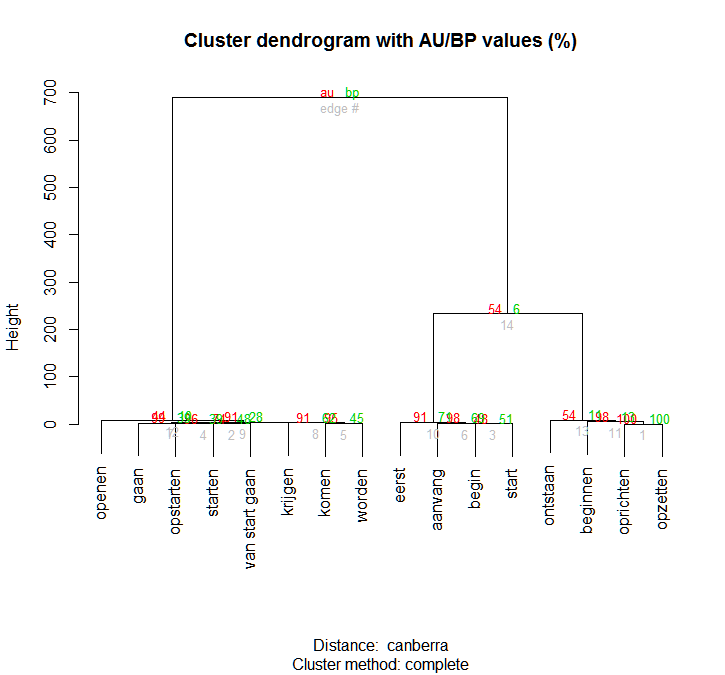
\includegraphics[height=.3\textheight]{figures/Vandevoorde2-img43.png}
\caption{\label{fig:key:43}  Canberra, Complete, on CA (14)}
\end{figure}

\begin{figure}
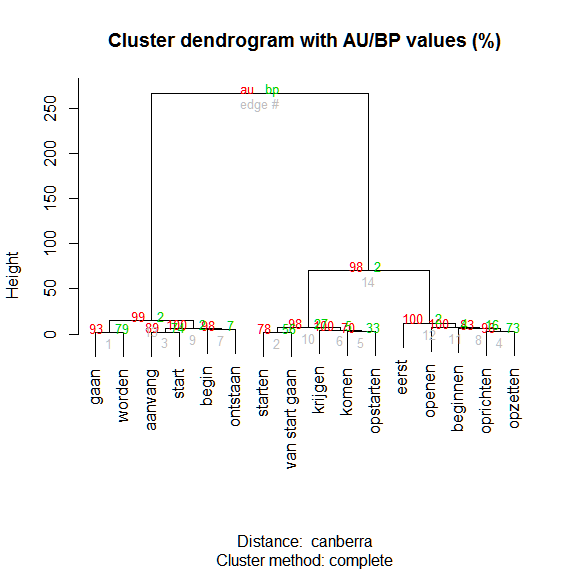
\includegraphics[height=.3\textheight]{figures/Vandevoorde2-img44.png}
\caption{\label{fig:key:44}  Canberra, Complete, on LSA (15)}
\end{figure}

\begin{figure}
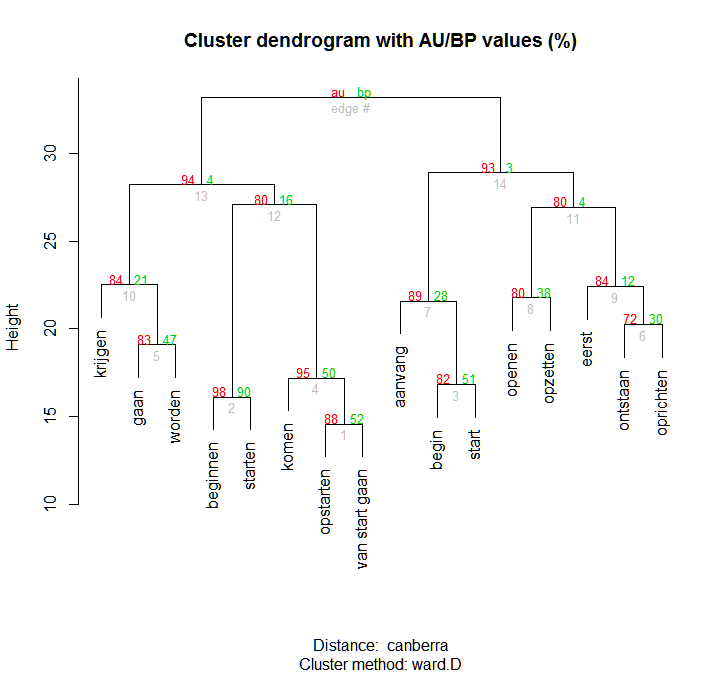
\includegraphics[height=.3\textheight]{figures/Vandevoorde2-img45.png}
\caption{\label{fig:key:45}  Canberra, Ward’s (16)}
\end{figure}

\begin{figure}
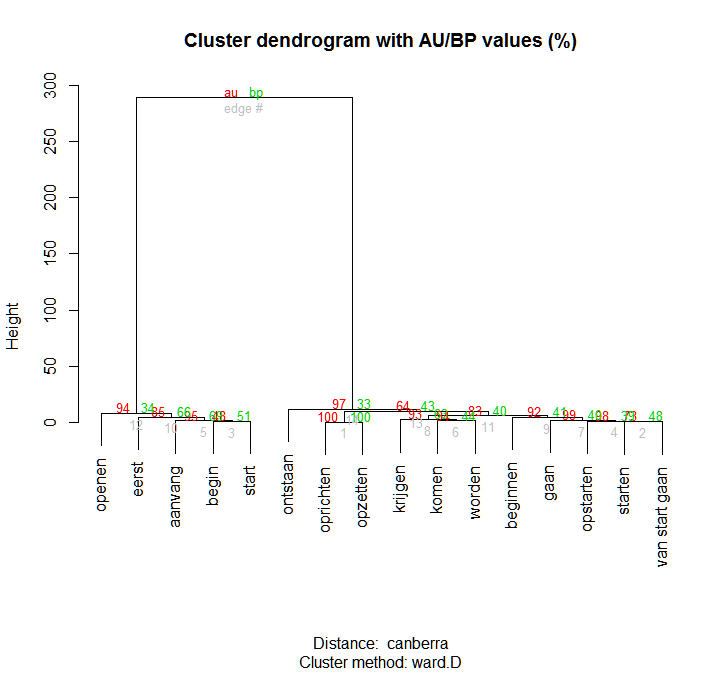
\includegraphics[height=.3\textheight]{figures/Vandevoorde2-img46.png}
\caption{\label{fig:key:46}  Canberra, Ward’s, on CA (17)}
\end{figure}

\begin{figure}
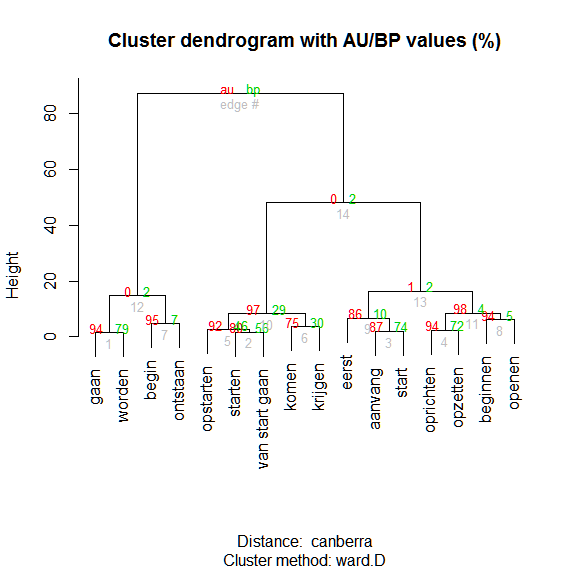
\includegraphics[height=.3\textheight]{figures/Vandevoorde2-img47.png}
\caption{\label{fig:key:47}  Canberra, Ward’s, on LSA (18)}
\end{figure}

\tabref{tab:key:13} (and the accompanying Figures 30 to 47\footnote{For each Figure, the number between brackets refers to the number of the combination in \tabref{tab:key:11} it represents. I will use these numbers to refer to the different combinations (not the Figure numbers).}), shows that combinations 8, 11, 12, 14, 15, 17 and 18 have an agglomerative coefficient higher than 0,80. It is noteworthy that only one combination with Euclidean distance reaches a satisfactory agglomerative coefficient. In addition, for the combinations with Canberra distance, none of the analyses carried out on the raw data display a satisfactory agglomerative coefficient.

Six out of nine combinations with Euclidean distance show a clear chaining effect (combinations 1, 2, 3, 4, 5 and 7). Combination 6 displays chaining on the higher edges of the dendrogram. Only combinations 8 and 9 (using Ward’s Minimum Variance Method) do not suffer from chaining. As for the combinations with Canberra distance, none of them displays clear chaining, although combinations 11, 14, 15 and 17 show space-dilation effects on the higher edges as well as chaining-effects on the lower edges. Combination 10 only shows some chaining on the higher edges. Combinations 12, 13, 16 and 18 show no effect of chaining nor space-dilation at all. Chaining and space-dilation effects seem not to be limited to the complete linkage algorithm but appear irrespective of the clustering algorithm.

For the combinations with Euclidean distance, all but two combinations display a high number of significant p-values (only combinations 6 and 9, carried out on the output of a LSA have less than 7 significant nodes). For the combinations with Canberra distance,we only two out of nine combinations have 7 or more significant p-values: combinations 14 and 15, both carried out with the complete linkage algorithm.

On the basis of the obtained values for each of the criteria in the comparison, it can be concluded that combinations 8 (Euclidean, Wards, on CA), 14 (Canberra, Complete, on CA) and 15 (Canberra, Complete, on LSA) are most likely to yield interpretable results for these data. Preference goes to combination 8, because no chaining was observed at all (in combinations 14 and 15 space-dilation in the high nodes and chaining in the low nodes was observed). In addition, this is the only combination with Ward’s Method, which is the more natural choice when one adheres a prototype-based view on clusters (as was explained in \sectref{sec:3.7.2.2}). On the basis of this comparison, it is decided to apply combination 8 (Euclidean, Wards, on CA) to all data sets of the case study of \textit{beginnen.}

The previous comparison also leads to some more general observations: when Euclidean distance is used, chaining effect, relatively high agglomerative coefficients (although lower than for Canberra) and a high number of significant p-values are more likely to appear. Combining Euclidean distance with Ward’s Method seems to avoid chaining effects. Canberra distance, on the other hand, avoids chaining effect, renders high agglomerative coefficients (except on raw data) but renders a low number of significant p-values. From the point of view of the clustering algorithms, it is noteworthy that combinations with the complete linkage algorithm usually display a high amount of significant p-values and that combinations with Ward’s Method are usually best at avoiding chaining effect (only combination 7 with Ward’s displays clear chaining). When the different spatial maps are taken as point of departure, it appears that analyses on the raw data render low agglomerative coefficients and that analyses on the CA are prone to chaining.


\section{Statistical approach of universals on the semantic level}
\label{sec:3.8}
In the previous section \sectref{sec:3.7}, I explained the different decisions that led me to choose HAC carried out on CA to visualize the semantic fields of translated and non-translated inchoativity in Dutch. This methodological development is my answer to the first research question “how to investigate semantic differences?”. In \chapref{sec:4}, the technique developed in the current chapter will be applied to the field of inchoativity in Dutch. In this way, the second research question: “are there any differences on the semantic level between translated and non-translated language?” will be answered, although of course limited to the differences between translated and non-translated Dutch within the field of inchoativity. However, before the results of the case study can be presented in \chapref{sec:4}, more theoretical reflection is needed with respect to the third research question: “if there are any differences between the fields of translated and non-translated Dutch inchoativity, can we ascribe them to any of the universal tendencies of translation?”. In the sub-sections \sectref{sec:3.8.1} and \sectref{sec:3.8.2} below, I will make a number of methodological and conceptual propositions that will enable me to investigate whether the presumed differences between translated and non-translated Dutch on the semantic level might be ascribed the following universal tendencies: levelling out – which has received very few attention from CBTS researchers (see \sectref{sec:2.2.2.4}) – or normalization and shining through – which take into account specific source and specific target language influence on translated language (see \sectref{sec:2.2.2.3}). For each of these universal tendencies, a difference will be furthermore made between the semasiological and the onomasiological perspective (see \sectref{sec:3.2}), leading to different operationalizations for comparison on the semantic level.

\subsection{Measuring prototypicality effects as a proxy for levelling out}
\label{sec:3.8.1}
Levelling out can be investigated by comparing the variation of a certain feature in translated language to the variation of the same feature in non-translated language (see \sectref{sec:2.2.2.4}). On the semantic level, levelling out can be examined on the semasiological level by comparing the variation of the feature \textit{meaning} \textit{distinctions} in translated language to its variation in non-translated language. For this particular case study, appearance of semantic levelling out on the semasiological level would imply that in translated language, \textit{beginnen} displays fewer meaning distinctions compared to non-translated language. Semantic levelling out could also be investigated on the onomasiological level by comparing the variation of the feature \textit{number} \textit{of} \textit{lexical} \textit{expressions} \textit{per} \textit{meaning} \textit{distinction} in translated language to its variation in non-translated language. For \textit{beginnen,} semantic levelling out on the onomasiological level would manifest itself through the use of fewer lexical expressions to express the different meanings of \textit{beginnen}.

Under the assumption that the meaning distinctions for \textit{beginnen} will be very subtle, I expect that the semantic variation between the fields of translated and non-translated Dutch inchoativity will be small and hence difficult to observe by mere inspection of the clusters in the dendrograms since these clusters are all on an equal par, i.e. they simply represent a partitioning of the lexemes. As a solution to this, I will measure the centrality of each of the meanings (represented as clusters) and focus on possible changes within their prototype-based organization. By determining which clusters are more central in the semantic space and which ones are more peripheral, changes in the prototype-based organization of the meanings within the semantic fields are assessed. Semasiological levelling out will consequently be investigated by looking at the prototype-based organization of the clusters within each dendrogram (SourceDutch, TransDutchENG and TransDutchFR). This will be done by comparing the distances-to-centroids of the clusters within each dendrogram (\sectref{sec:3.8.1.1}). Onomasiological levelling out will be investigated by comparing the prototype-based organization of the lexemes in each cluster and for each field (SourceDutch, TransDutchENG and TransDutchFR) to each other. This will be done by evaluating the distance of each lexeme to the centroid (considered as the abstract prototype) of the cluster (the meaning distinction) it belongs to (\sectref{sec:3.8.1.2}).

In \sectref{sec:3.8.1.3} I will further explore how centroids and medoids may represent different views on prototypes. In addition, each cluster in a dendrogram will also receive a meta-label as a solution to capture the specific meaning distinction of each cluster (\sectref{sec:3.8.1.4}).

\subsubsection{Organization of clusters within each dendrogram}
\label{sec:3.8.1.1}  
The prototype-based organization of the clusters within each dendrogram will be explored by assessing the distance of each cluster’s center (its centroid) to the zero-point of the semantic space. Centroids correspond to the average of all points in the cluster \citep[494]{tan_introduction_2006}. They can be calculated on the resulting coordinates of the CA (recall that the output of the CA will be used as input for the HAC). The zero-point or origin of a semantic space corresponds to the weighted mean of the columns and of the rows (they are superposed and calibrated on the zero-point). If a data point is situated close to the origin, this implies that its weighted mean is close to the overall weighted mean. The data point can hence be considered as ‘central’ in the spatial map, and its profile will be rather resembling to other, equally central points in the spatial map. If Lakoffs idea (1987, cited by \citealt{tyler_semantics_2003}) that lexical categories and polysemy networks are structured with respect to their prototypical meanings is accepted, and if Dyvik’s basic idea that “semantically closely related words ought to have strongly overlapping sets of translations” is equally accepted, from which it follows that strongly overlapping sets of translation ought to reveal semantic relatedness; then this leads to the assumption that the central sphere of a spatial map – close to the zero-point or origin – can be considered as the prototypical center. As a consequence, the data points (be it centroids or lexemes) which find themselves in or close to this central sphere can then be considered as prototypical points in the semantic space. The distances of the clusters’ centroids to the zero-point (the prototypical center) of the semantic space they belong to can be informative about the more prototypical or more peripheral position of each cluster (meaning distinction) in the semantic space (the semantic field it belongs to).

The coordinates of the cluster center (the centroid) are calculated on the output of the CA (i.e. the coordinates of the CA) with the built-in function centers\_ca() from the svs{}-package. Next, the Euclidean distance from each centroid to the zero-point of the semantic space is calculated with the helper function dist\_wrt() from svs. Finally, the distances of the centroids to the origin of the semantic space are visualized with a dot chart. The example in \figref{fig:key:48} shows the distance of each of the clusters in the HAC visualization for SourceDutch to the origin of the semantic space. Since the zero-point of the semantic space is held to be the prototypical center, clusters that are closer to the zero-point of the semantic space are considerd as more prototypical and clusters further away from the zero-point as more peripheral. 

\begin{tabular}{ll}
\lsptoprule
Cluster 6 & eerst\\
Cluster 5 & krijgen, komen, worden\\
Cluster 4 & ontstaan, openen\\
Cluster 3 & Starten, van start gaan, opstarten, beginnen, gaan\\
Cluster 2 & aanvang, begin, start\\
Cluster 1 & opzetten, oprichten\\
\lspbottomrule
\end{tabular}\todo{Where does this table belong?}

\begin{figure}
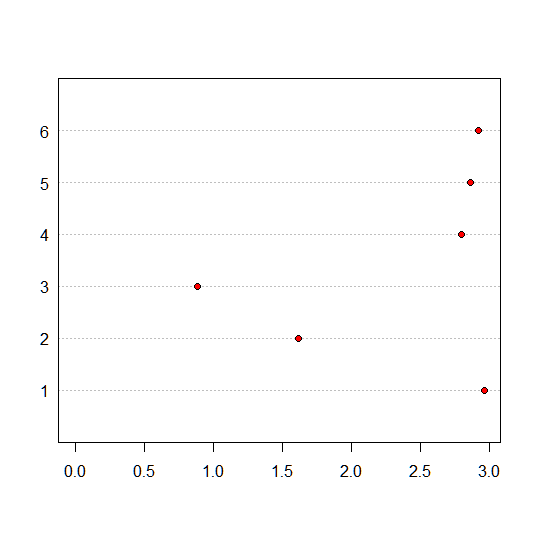
\includegraphics[height=.3\textheight]{figures/Vandevoorde2-img48.png}
\caption{\label{fig:key:48}  Dot chart presenting the distance of the cluster centroids to the zero-point of the semantic space of SourceDutch}
\end{figure}

\subsubsection{Organization of the lexemes within each cluster}
\label{sec:3.8.1.2}
The prototype-based organization of the different items (lexemes) within each cluster can equally be assessed with centroids by measuring the distance of each lexeme to the centroid of the cluster it belongs to. The Euclidean distance from the lexemes to each of the cluster centroids can be calculated with the function dist\_wrt\_centers() from svs and visualized in a dot chart (an example can be found in \figref{fig:key:49}). The distance of the lexemes to the centroid (the average of all points in the cluster) of the cluster they belong to can be used to explore which lexical items are more prototypical expressions of the particular meaning distinction (indicated by the cluster) and which ones are more peripheral. For the example in \figref{fig:key:49}, we see that \textit{starten} and \textit{beginnen} are the lexemes situated closest to the centroid of the cluster they belong to, implying that they are closest the abstract prototype contained in the centroid (see \sectref{sec:3.7.3.3}).

\begin{figure}
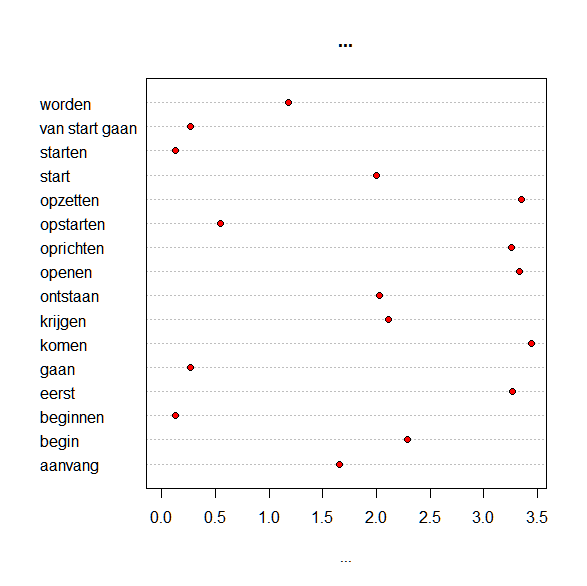
\includegraphics[height=.3\textheight]{figures/Vandevoorde2-img49.png}
\caption{\label{fig:key:49}  Dot chart representing the distance of the lexemes to the centroid of cluster n°4 for SourceDutch}
\end{figure}

The stability of the cluster membership of each lexeme can also be determined on the basis of this analysis. HAC is categorized as hard clustering, which means that each object in the analysis can be assigned to only one cluster (in contrast to fuzzy clustering, which can reveal the degree of membership of an object to a cluster). By looking at the distance of the lexemes to their cluster’s centroid, the hard clustering is somewhat nuanced. The positions of the lexemes with respect to their centroid may show that some lexemes are ‘hesitant’ between two clusters, and their assignment to a particular cluster is not as straightforward and clear-cut (as hard) as the dendrogram structure would have suggested. The centroid itself, however, is not a meaningful point\footnote{Manning and Schütze (1999, 516) point out that the centroid “is in most cases not identical to any of the objects”.} since it is the average of all points. Alternatively, it is possible to compute the medoid for each cluster, which is the particular point in the cluster with the smallest average distance to all other points \citep[164]{divjak_structuring_2010}. Everitt et al. note that the term medoid was coined by \citet{kaufman_finding_1990} by analogy with calling the group mean the centroid. The medoid “can be interpreted as a representative object or exemplar of the group” \citep[113]{everitt_cluster_2011} and is necessarily one object in the cluster; this object can then be considered as the “prototypical class member” \citep[516]{manning_foundations_1999} in a cluster. The medoid can be calculated with the pam(){}-function in R (‘Partitioning around Medoids’).

For each cluster analysis, I will calculate both the medoid of each cluster as well as the distance of each lexeme to the centroid of the cluster it belongs to. Both measures seem to have their own advantage(s). The distances of each of the lexemes to the centroid allow to better understand the organization of the lexemes in a cluster as a ‘continuum’ with some lexemes closer to the centroid (the most central ones) and others further away from the centroid (the most peripheral ones). The medoid on the other hand indicates one particular lexeme but is less informative about the structure of the cluster. If the medoid happens to be different from the lexeme closest to the centroid, this could indicate tension between several prototypical expressions.

\subsubsection{Centroids and medoids: different views on prototype}
\label{sec:3.8.1.3}
Both measures (distance to the centroid and medoid) can be used to determine which lexical item in each cluster can be considered as the most prototypical expression of that cluster (the particular meaning distinction indicated by the cluster). However, distance to centroid and medoid could be seen as representing two different views on prototypes.

Descriptions of the prototype-based organization of the lexical items in a cluster which rely on the distance of the items to the centroid imply that prototype is regarded as a “summary representation” \citep[42]{murphy_big_2004}, meaning that “an entire category is represented by a unified representation” where “[t]he concept is represented as features that are usually found in the category members, but some features are more important than others” (Murphy, Ibid.)\todo{Fix Ref}. Because such a summary representation is (always) abstract, it would strictu sensu not be possible to capture the summary representation within only one lexeme of the cluster (since the prototype would be an abstract sum of features). However, it is also possible to consider the lexeme closest to the centroid as the one that – in the best way possible – reunites the features usually found in the category members, without considering it as the ‘ideal member’ (the ideal member would be the centroid itself, which does not coincide with any of the cluster’s members). Hence, the lexeme closest to the centroid can be seen as the best possible representation of the abstract prototype contained in the centroid. If the medoid of a cluster is regarded as the prototype of the cluster it belongs to (the particular meaning distinction), this would correspond to Murphy’s “best example idea” (2004, 42)\todo{Fix ref}, where “a single prototype could represent a whole category” (Murphy, Ibid.)\todo{Fix ref}. The medoid then indicates the best example as the prototype of the cluster it belongs to.

\subsubsection{Manual assignment of meta-labels}
\label{sec:3.8.1.4}  
A meta-label will be assigned to each cluster in the dendrogram in an effort to name the specific meaning distinction indicated by the cluster. There are several options to arrive at such a label. Firstly, either the lexeme closest to the centroid or the medoid of each cluster can be selected as its meta-label. However, since only 16 lexemes will be making up the dendrograms, several small clusters are to be expected (with 3 or fewer members). Indicating one of the few lexemes in such a small cluster as its meta-label will most likely not have much informative value with respect to the specific meaning distinction of that cluster.

Secondly, other quantitative techniques can be applied in an attempt to provide supplementary information about each cluster. This would, however, require an expansion of the amount and nature of annotated data in the data sets. It is possible, for instance, to carry out a supplementary annotation (e.g. of contextual information) and to add this information to the analysis. One possibility would be to apply a behavioral profiling \citep{divjak_ways_2006, divjak_clusters_2008, evans_behavioral_2009} to the resulting data sets (which would consist in coding each item occurring in each of the sentences for a number of variables, known as ID tags)\footnote{While such an analysis would have certainly yielded new insights, it could not be carried out within the scope of this study.}. A third option is to manually label each cluster in an attempt to capture its specific meaning distinction via a more qualitative analysis of each cluster. For this study, I will opt for such a manual assignment task, which will consist in a thorough inspection of each cluster in a dendrogram. The assigned meta-label will combine information of three types of sources: corpus examples from the DPC containing the lexemes which make up a cluster, attestations in reference works and information from the lexical database Cornetto \citep{vossen_cornetto_2008, spyns_cornetto:_2013}. Cornetto is a lexical data base for Dutch which consists of two existing semantic resources (Dutch Word Net and Referentiebestand Nederlands). It was created within the same project (STEVIN) as the Dutch Parallel Corpus that we are using in this study (see \sectref{sec:3.3}). The semantic properties of words are described in Cornetto by the categories Sentiment (with labels such as ‘positive’ and ‘negative’), Pragmatics (including usage information about domain, chronology, connotation, geography and register), Semantics (with specific values for each part-of-speech) and SenseExamples (information about the combinatoric properties). The integration of the variety of semantics-related information obtained via Cornetto could also have been done in a quantitatively more robust way, rather than via the qualitative analysis I propose\footnote{A quantitatively more robust way of integrating this variety of informative semantics-related labels into the analysis would be to manually tag the resulting data sets of the SMM++ with the semantic information from Cornetto and carry out an analysis using those tags as variables (as an alternative analysis to the clustering on the basis of translations/source language lexemes). Another option would be to add the information of these semantics-related labels as supplementary points to a Correspondence Analysis based on the translational data. Thirdly, one could also envisage to use the previously obtained translational information as an additional tag and carry out a cluster analysis using both the semantics-related labels and the translations as variables.}. However, such an operation would have (again) required an expansion of the amount and nature of annotated data (the resulting data sets of the SMM++ would need supplementary annotation with the semantic information from Cornetto before an analysis using those tags as variables could be carried out). Although such an analysis would definitely enrich the dendrograms and consequently allow for more fine-grained descriptions of the clusters – while simultaneously adding interpretative power – I did not further investigate this option within the purview of this study, mainly because the main focus of this book is to explore as many potentialities as possible of translational data ‘alone’ for semantic description, without using any additional annotative information in the analysis.

\subsection{Semantic fields of commencer and to begin}
\label{sec:3.8.2}  
The investigation of semantic normalization and shining through on both the semasiological and the onomasiological level requires a number of additional visualizations.

On the semasiological level, target language influence on the meaning distinctions in translated Dutch inchoativity (\textbf{semasiological} \textbf{normalization}) will be investigated by comparing the meaning distinctions in translated Dutch to those present in non-translated Dutch, for which the visualizations are available the basis of the methodology clarified above. Source language influence on the meaning distinctions in translated Dutch inchoativity (\textbf{semasiological} \textbf{shining} \textbf{through}) will be investigated by comparing the meaning distinctions in translated Dutch to those present in the source languages. This will be done by visualizing the semantic fields of the closest equivalents of \textit{beginnen} in the source languages of TransDutch\textsubscript{ENG} and TransDutch\textsubscript{FR}, viz. SourceEnglish \textit{to} \textit{begin} and SourceFrench \textit{commence}r. The meaning distinctions in the fields of \textit{to} \textit{begin} and \textit{commencer} are compared to those present in TransDutch\textsubscript{ENG} and TransDutch\textsubscript{FR} respectively, to see whether the specific meaning distinctions within the semantic fields of SourceEnglish and SourceFrench might have influenced the organization of the meaning distinctions in TransDutch\textsubscript{ENG} and TransDutch\textsubscript{FR}. The resulting semantic spaces of inchoativity in French and English are independent of TransDutch and correspond to the second T-images\footnote{Note that for \textit{commencer} and \textit{to} \textit{begin}, only one mirroring can be carried out (i.e. with a single language B– Dutch) since the DPC does not contain the translation directions French-English, English-French. Consequently, the data sets for the \textit{second} \textit{T-images} are based on a single data set (compared to the second T-image data set for SourceDutch, which consists of the combined data of the second T-image of beginnen\textsubscript{FR} and beginnen\textsubscript{ENG} ).} of \textit{commencer} and of \textit{to} \textit{begin.}

With \textbf{onomasiological} \textbf{normalization,} I refer to the possible influence of non-translated Dutch on the prototype-based organization of the lexemes within each meaning distinction of \textit{beginnen} in translated Dutch. This can be assessed by comparing the prototype-based organization of the lexemes in each meaning distinction in SourceDutch to the organization of the lexemes in each meaning distinction in TransDutch\textsubscript{ENG} and TransDutch\textsubscript{FR}. If the same organization of lexemes appears in TransDutch\textsubscript{ENG} and TransDutch\textsubscript{FR} and this organization is similar or identical to the organization in SourceDutch, there is a good chance that the TransDutch fields are ‘conforming’ to the SourceDutch field, yielding evidence for onomasiological normalization. \textbf{Onomasiological} \textbf{shining} \textbf{through} would manifest itself as an influence of the source language on the organization of the lexemes within each meaning distinction of \textit{beginnen} in translated Dutch. In order to asses such an influence, the English and French source language lexemes – which determine the clustering of the Dutch lexemes in TransDutch\textsubscript{ENG} and TransDutch\textsubscript{FR} into specific meaning distinctions – will be visualized together with the Dutch target language lexemes. In this way, it can be observed how the specific organization of the lexical items within the clusters – with each cluster representing a particular meaning distinction of \textit{beginnen} – is possibly influenced by a specific underlying source language lexeme. In order to obtain a simultaneous representation of the source and target language lexemes in a single semantic space, I will carry out a Multiple Correspondence Analysis on a Burt table \citep{greenacre_simple_2006, greenacre_correspondence_2007}. Burt tables are generalizations of ordinary frequency tables with row and column categories, in that they cross all categories as rows with all categories as columns. The advantage of a Multiple Correspondence Analysis on a Burt table is that distances can be computed, not only between (Dutch) target lexemes themselves, but also between target lexemes and source lexemes so that both source language lexemes and target language lexemes are represented in a single space. This MCA on a Burt table is subsequently visualized with a HAC, enabling us to visually inspect which Dutch target lexemes are associated with which French or English source lexemes.

\section{Conclusion}
\label{sec:3.9}  
In this chapter, I have proposed a methodology to investigate semantic differences between translated and non-translated language. The method is an extension of an existing method (the SMM); it is corpus-based, uses statistical visualization techniques and consists of two parts (two extensions to the SMM). The first extension allows the potential user of the method to select candidate-lexemes for a semantic field. This selection mechanism (retrieval method) is translation-driven and uses the different translational statuses (either source or target language) of parallel corpus data. The second extension to the SMM proposes a way to visually inspect the retrieved data sets via a combination of CA and HCA. First, CA is applied in order to construct a low-dimensional semantic space of the data. Second, HAC is applied in order to distinguish clusters of lexemes within the semantic spaces. The technique is calibrated by the Euclidean distance measure and Ward’s Minimum Variance Method as the amalgamation rule. In this methodological chapter, the way was furthermore paved to investigate levelling out, shining through and normalization on both the semasiological and the onomasiological level.

In the next chapter, I will apply the two extensions of the SMM to the semantic field of inchoativity in Dutch. The comparison of different visualizations representing the semantic fields of SourceDutch, TransDutch\textsubscript{ENG} and TransDutch\textsubscript{FR} will enable me to tackle the second question I aim to answer with this study: “Are there any of the (universal) tendencies of translation that also apply to the semantic level?” as well as the third one: “If there are differences on the semantic level, can we ascribe them to any of the (universal) tendencies of translation?”.